本报告复盘 Unitree H1 右髋俯仰与右膝关节输入域 EID 控制实验，围绕软件输入端等效扰动下的误差收益、力矩代价、参数敏感性和候选机理展开分析。报告内容包括实机日志统计、频谱与恢复段分析、\texttt{eta\_u} 与软件扰动的关系、力矩项分解、Pareto 权衡、MuJoCo 机制矩阵、局部离散辨识和增广闭环频响。

实验数据来自 2026-06-23 的右髋-右膝台架实验，以及下文定义的两类软件输入端等效扰动实验。MuJoCo 与局部线性模型结果用于候选压缩和机理解释，不能替代实机安全裕度、实机稳定性证明或真实外部物理接触力下的抗扰验证。

\section{0. 独立阅读所需定义}\label{ux72ecux7acbux9605ux8bfbux6240ux9700ux5b9aux4e49}

为使后续结果可直接复核，本节统一给出缩写、参数名和候选名的含义；后文表格中的 \texttt{O4}、\texttt{U1}、\texttt{A}、\texttt{B}、\texttt{E} 等均按本节定义阅读。

\subsection{0.1 控制对象与控制器}\label{ux63a7ux5236ux5bf9ux8c61ux4e0eux63a7ux5236ux5668}

实验对象是 Unitree H1 的右髋俯仰关节和右膝关节。报告中的 PD 指电机位置模式基线：控制器下发参考位置、参考速度和电机侧 \texttt{kp/kd}。报告中的 EID 指``包含解析逆模型的输入域 EID 整体结构''，不是单独的扰动估计模块。

每个关节维护标称预测状态 \texttt{xhat} 和 EID 估计量 \texttt{eta}。EID 估计量一方面形成中心反馈状态，

\[
\bar{x}=\hat{x}+\eta,
\]

另一方面通过输入补偿增益 \texttt{K\_u} 映射为输入端补偿力矩，

\[
\eta_u=K_u\eta.
\]

最终力矩由解析逆模型前馈、输入补偿和围绕中心反馈状态的 PD 修正共同构成：

\[
u=u^\star-\eta_u+K(r-\bar{x}).
\]

因此，\texttt{K\_o} 在本报告中表示 EID 估计量对状态残差的响应强度，\texttt{K\_u} 表示估计量映射到输入端补偿力矩的强度。\texttt{eta} 与 \texttt{eta\_u} 是控制器内部状态修正量和输入补偿量，不能直接等同于真实外力或真实外部扰动力矩。

\subsection{0.2 实机实验缩写}\label{ux5b9eux673aux5b9eux9a8cux7f29ux5199}

\begin{longtable}[]{@{}
  >{\raggedright\arraybackslash}p{(\linewidth - 6\tabcolsep) * \real{0.2500}}
  >{\raggedright\arraybackslash}p{(\linewidth - 6\tabcolsep) * \real{0.2500}}
  >{\raggedright\arraybackslash}p{(\linewidth - 6\tabcolsep) * \real{0.2500}}
  >{\raggedright\arraybackslash}p{(\linewidth - 6\tabcolsep) * \real{0.2500}}@{}}
\toprule\noalign{}
\begin{minipage}[b]{\linewidth}\raggedright
缩写
\end{minipage} & \begin{minipage}[b]{\linewidth}\raggedright
本报告中的含义
\end{minipage} & \begin{minipage}[b]{\linewidth}\raggedright
控制器/扫描对象
\end{minipage} & \begin{minipage}[b]{\linewidth}\raggedright
扰动与重复
\end{minipage} \\
\midrule\noalign{}
\endhead
\bottomrule\noalign{}
\endlastfoot
P2D & P2 的双关节软件力矩扰动补充实验 & PD 与 EID 对比 & 右髋叠加 \texttt{+6\ N\ m}、右膝叠加 \texttt{-4\ N\ m} 的平滑力矩脉冲，每组 5 次 \\
P4D \texttt{K\_o} 扫描 & P4 的带软件扰动观测器倍率扫描 & EID，改变观测器倍率 \texttt{s\_o} & 使用与 P2D 相同的软件力矩扰动，每组 3 次 \\
P4D \texttt{K\_u} 扫描 & P4 的带软件扰动输入补偿倍率扫描 & EID，改变输入补偿倍率 \texttt{s\_u} & 使用与 P2D 相同的软件力矩扰动，每组 3 次 \\
\end{longtable}

P2D 和 P4D 的扰动窗口均为 \texttt{4.0\ \textless{}=\ t\_rel\ \textless{}\ 5.4\ s}，其中 \texttt{4.2-\/-5.2\ s} 为恒定扰动平台段，\texttt{5.4-\/-7.4\ s} 为恢复观察段。后文的``完整扰动窗口''指日志覆盖完整 \texttt{4.0-\/-5.4\ s} 窗口。

\subsection{0.3 参数倍率与 O/U 命名}\label{ux53c2ux6570ux500dux7387ux4e0e-ou-ux547dux540d}

为避免把绝对增益和扫描倍率混在一起，本文用 \texttt{s\_o} 表示观测器倍率，用 \texttt{s\_u} 表示输入补偿倍率：

\[
K_o=s_oK_o^{\rm nom},\qquad
K_o^{\rm nom}=
\begin{bmatrix}
0.8 & 0\\
0 & 0.2
\end{bmatrix},
\]

\[
K_u=s_uK_u^{\rm nom},\qquad
K_u^{\rm nom}=
\begin{bmatrix}
12.0 & 1.0
\end{bmatrix},
\qquad \alpha=0.85.
\]

O0--O5 是 P4/P4D 的观测器倍率组。除非特别说明，O 组扫描中 \texttt{s\_u=1.0}：

\begin{longtable}[]{@{}lrrrl@{}}
\toprule\noalign{}
组别 & \texttt{s\_o} & \texttt{observer\_gain\_q} & \texttt{observer\_gain\_dq} & 含义 \\
\midrule\noalign{}
\endhead
\bottomrule\noalign{}
\endlastfoot
O0 & 0.00 & 0.0 & 0.00 & 关闭观测器增益 \\
O1 & 0.25 & 0.2 & 0.05 & 低观测器倍率 \\
O2 & 0.50 & 0.4 & 0.10 & 中低观测器倍率 \\
O3 & 0.75 & 0.6 & 0.15 & 中高观测器倍率 \\
O4 & 1.00 & 0.8 & 0.20 & 标称观测器倍率 \\
O5 & 1.25 & 1.0 & 0.25 & 高观测器倍率 \\
\end{longtable}

U1--U4 是 P4/P4D 的输入补偿倍率组。除非特别说明，U 组扫描中 \texttt{s\_o=1.0}：

\begin{longtable}[]{@{}lrrrl@{}}
\toprule\noalign{}
组别 & \texttt{s\_u} & \texttt{ku\_q} & \texttt{ku\_dq} & 含义 \\
\midrule\noalign{}
\endhead
\bottomrule\noalign{}
\endlastfoot
U1 & 0.50 & 6.0 & 0.50 & 弱输入补偿 \\
U2 & 0.75 & 9.0 & 0.75 & 中弱输入补偿 \\
U3 & 1.00 & 12.0 & 1.00 & 标称输入补偿 \\
U4 & 1.25 & 15.0 & 1.25 & 强输入补偿 \\
\end{longtable}

注意：P4D 实机中，O5 和 U1 是两条一维扫描上的不同实测组。\texttt{O5+U1} 是组合候选，表示同时使用 \texttt{s\_o=1.25} 和 \texttt{s\_u=0.5}；它不是本轮已经实测的 P4D 组，需要下一轮单独上机验证。

\subsection{0.4 下一轮候选矩阵命名}\label{ux4e0bux4e00ux8f6eux5019ux9009ux77e9ux9635ux547dux540d}

MuJoCo 机制矩阵和下一轮实机计划使用 A/B/C/D/E 等候选名。所有候选默认固定弱输入补偿 \texttt{s\_u=0.5}，区别主要在逐关节观测器倍率：

\begin{longtable}[]{@{}
  >{\raggedright\arraybackslash}p{(\linewidth - 8\tabcolsep) * \real{0.1765}}
  >{\raggedright\arraybackslash}p{(\linewidth - 8\tabcolsep) * \real{0.1765}}
  >{\raggedleft\arraybackslash}p{(\linewidth - 8\tabcolsep) * \real{0.2353}}
  >{\raggedleft\arraybackslash}p{(\linewidth - 8\tabcolsep) * \real{0.2353}}
  >{\raggedright\arraybackslash}p{(\linewidth - 8\tabcolsep) * \real{0.1765}}@{}}
\toprule\noalign{}
\begin{minipage}[b]{\linewidth}\raggedright
候选名
\end{minipage} & \begin{minipage}[b]{\linewidth}\raggedright
配置含义
\end{minipage} & \begin{minipage}[b]{\linewidth}\raggedleft
髋 \texttt{s\_o}
\end{minipage} & \begin{minipage}[b]{\linewidth}\raggedleft
膝 \texttt{s\_o}
\end{minipage} & \begin{minipage}[b]{\linewidth}\raggedright
证据角色
\end{minipage} \\
\midrule\noalign{}
\endhead
\bottomrule\noalign{}
\endlastfoot
A 或 \texttt{A\_O4U1} & \texttt{O4+U1} 保守基线 & 1.00 & 1.00 & 已有实机依据，下一轮同批复测基线 \\
B 或 \texttt{B\_HipUp} & 只提高髋观测器倍率 & 1.25 & 1.00 & MuJoCo 迹象，待实机验证 \\
C & 只降低膝观测器倍率 & 1.00 & 0.75 & 下一轮 2x2 矩阵候选，待实机验证 \\
D 或 \texttt{D\_HipUpKneeDown} & 髋增强、膝减弱 & 1.25 & 0.75 & 非对称调参假设的直接验证点 \\
E 或 \texttt{O5+U1} / \texttt{O5U1} & 髋膝共同提高观测器倍率，同时保持弱输入补偿 & 1.25 & 1.25 & 误差优先候选，待实机验证 \\
\texttt{KneeVelDown} & 只降低膝速度观测器通道，膝位置通道保持 1.00 & 髋 1.00 & 膝位置 1.00，膝速度 0.75 & 判断膝力矩活动是否主要来自速度残差通道 \\
\end{longtable}

\subsection{0.5 指标与符号}\label{ux6307ux6807ux4e0eux7b26ux53f7}

RMSE 是均方根误差，越小表示越接近参考目标。髋误差为 \texttt{e\_hip=q\_ref,hip-q\_hip}，膝误差为 \texttt{e\_knee=q\_ref,knee-q\_knee}。协调误差定义为

\[
e_{\rm coord}=e_{\rm hip}-e_{\rm knee},
\]

用于衡量右髋和右膝之间的相对运动是否被控制器破坏。\texttt{tau\_est} 表示执行器反馈/估计力矩，\texttt{Delta\ tau\_est} 表示相邻采样点之间的 \texttt{tau\_est} 变化量，用于描述力矩粗糙度或高频活动。\texttt{combined\_flags=4} 在 MuJoCo 表格中表示该仿真 case 出现了限幅/饱和类标志，因此 MuJoCo 排名不能直接当作实机安全结论。

\section{摘要}\label{ux6458ux8981}

本报告完成了 P2D/P4D 频谱分析、恢复段统计、\texttt{eta\_u} 与软件扰动对齐、力矩项分解、多目标 Pareto、真实 C++ stepper 的 MuJoCo 结构消融、残差 \texttt{lambda} 扫描，以及基于 MuJoCo 日志辨识的局部增广闭环频响。综合这些结果，核心结论如下。

\begin{enumerate}
\def\labelenumi{\arabic{enumi}.}
\tightlist
\item
  现有实机支持 EID 在 P2D 软件输入端等效扰动下有\textbf{部分抗扰收益}：髋窗口 RMSE 降低 18.2\%，协调窗口 RMSE 降低 6.1\%；但膝窗口 RMSE 上升 10.0\%，且髋/膝 \texttt{tau\_est} RMS 与 \texttt{Delta\ tau\_est} RMS 均增加。因此不能写成 EID 全指标优于 PD。
\item
  当前 P4D 只证明``髋膝共同增大 \texttt{K\_o} 时窗口 RMSE 下降''，不能直接证明``髋 \texttt{K\_o} 增大、膝 \texttt{K\_o} 降低''的逐关节非对称调参已经成立。
\item
  \texttt{O5+U1} 不是已经实测的组合。P4D 的 O5 是 \texttt{(s\_o=1.25,\ s\_u=1.0)}，U1 是 \texttt{(s\_o=1.0,\ s\_u=0.5)}；\texttt{O5+U1=(s\_o=1.25,\ s\_u=0.5)} 需要下一轮单独验证。
\item
  MuJoCo 机制矩阵显示，E（\texttt{O5+U1}，髋膝共同高观测器倍率并保持弱输入补偿）相对 A（\texttt{O4+U1} 保守基线）的协调 RMSE 降低约 2.32\%，但膝 \texttt{Delta\ tau\_total} RMS 上升约 0.82\%；B（只提高髋观测器倍率）只带来约 0.54\% 的协调 RMSE 下降，但力矩代价更保守；D（髋增强、膝减弱）和 \texttt{KneeVelDown} 能降低膝力矩变化量约 1.3\%--1.4\%，代价是协调 RMSE 变差约 2.5\%--2.8\%。
\item
  真实 stepper 结构消融显示，\texttt{K\_u\ eta} 输入补偿通道不是当前窗口 RMSE 的主要杠杆；完整 EID 的主要动态变化来自 \texttt{xbar=\textbackslash{}hat\{x\}+\textbackslash{}eta} 反馈中心和残差定义。因此低 \texttt{K\_u} 应作为保守补偿基线，而不是解决真实力矩波动的主要手段。
\end{enumerate}

下一轮实机应以 A（\texttt{O4+U1}，标称观测器倍率 + 弱输入补偿）作为已实测保守基线，优先验证 B（只提高髋观测器倍率）和 E（\texttt{O5+U1}，髋膝共同提高观测器倍率）；若要直接回答非对称调参假设，则执行 A/B/C/D 的最小 2x2 矩阵。D（髋增强、膝减弱）或 \texttt{KneeVelDown} 应作为``膝力矩活动约束''的机理验证点，而不是预写成最优参数。

\section{1. 分析项目与证据边界}\label{ux5206ux6790ux9879ux76eeux4e0eux8bc1ux636eux8fb9ux754c}

本报告将实机日志、离线分析、MuJoCo 机制筛查和局部线性模型分层处理。各层证据的用途和边界如下。

\begin{longtable}[]{@{}
  >{\raggedright\arraybackslash}p{(\linewidth - 6\tabcolsep) * \real{0.2500}}
  >{\raggedright\arraybackslash}p{(\linewidth - 6\tabcolsep) * \real{0.2500}}
  >{\raggedright\arraybackslash}p{(\linewidth - 6\tabcolsep) * \real{0.2500}}
  >{\raggedright\arraybackslash}p{(\linewidth - 6\tabcolsep) * \real{0.2500}}@{}}
\toprule\noalign{}
\begin{minipage}[b]{\linewidth}\raggedright
分析项目
\end{minipage} & \begin{minipage}[b]{\linewidth}\raggedright
当前状态
\end{minipage} & \begin{minipage}[b]{\linewidth}\raggedright
主要结果/产物
\end{minipage} & \begin{minipage}[b]{\linewidth}\raggedright
证据边界
\end{minipage} \\
\midrule\noalign{}
\endhead
\bottomrule\noalign{}
\endlastfoot
P2D/P4D 频谱分析 & 已完成 & P2D PD/EID 频谱、P4D O4/O5/U1/U4 候选频谱、MuJoCo PSD/coherence/经验 FRF & 闭环日志频谱和经验 FRF 只能解释现象，不是严格开环辨识 \\
恢复段统计补充 & 已完成 & P2D 扰动前/扰动窗口/恢复段统计，P4D 候选窗口统计 & 恢复段仍基于软件输入端等效扰动 \\
控制器机理拆解与消融仿真 & 已完成真实 C++ stepper 版本 & \texttt{eid\_mode} 四模式结构消融 & 仿真中所有 case 均出现限幅/饱和类 \texttt{combined\_flags=4}，不能替代实机安全裕度 \\
离散时间增广闭环与频响分析 & 已完成 MuJoCo 日志辨识版本 & 局部离散 plant、局部增广闭环极点、扰动到误差 Bode、噪声到控制奇异值 & 只能说明局部模型趋势，不能证明实机全局稳定 \\
残差定义与 \texttt{K\_u} 通道可辨识性 & 已完成 & \texttt{residual\_eta\_lambda} 扫描、\texttt{eta\_u} 对齐、力矩项分解 & \texttt{lambda=0} 等候选不能直接上机，需要叠加噪声和更严格限幅后再筛 \\
多目标/Pareto 设计 & 已完成 & 实物日志 Pareto、权重敏感性、MuJoCo 候选 Pareto & Pareto 用于候选压缩，最终排序必须以同批实机重复和饱和约束为准 \\
\end{longtable}

\section{2. 证据等级与报告边界}\label{ux8bc1ux636eux7b49ux7ea7ux4e0eux62a5ux544aux8fb9ux754c}

\begin{longtable}[]{@{}
  >{\raggedright\arraybackslash}p{(\linewidth - 4\tabcolsep) * \real{0.3333}}
  >{\raggedright\arraybackslash}p{(\linewidth - 4\tabcolsep) * \real{0.3333}}
  >{\raggedright\arraybackslash}p{(\linewidth - 4\tabcolsep) * \real{0.3333}}@{}}
\toprule\noalign{}
\begin{minipage}[b]{\linewidth}\raggedright
等级
\end{minipage} & \begin{minipage}[b]{\linewidth}\raggedright
本报告允许的表述
\end{minipage} & \begin{minipage}[b]{\linewidth}\raggedright
对应内容
\end{minipage} \\
\midrule\noalign{}
\endhead
\bottomrule\noalign{}
\endlastfoot
已由实机支持 & P2D/P4D 日志直接支持的结论 & P2D 部分抗扰收益；P4D 共同 \texttt{K\_o} 扫描；\texttt{K\_u} 扫描收益有限 \\
离线日志补充 & 对已有实机日志的解释 & 频谱、恢复段、\texttt{eta\_u} 对齐、力矩项分解、Pareto \\
MuJoCo 迹象 & 用于压缩候选和解释机制 & B（只提高髋观测器倍率）、D（髋增强、膝减弱）、E（\texttt{O5+U1}）、\texttt{KneeVelDown}、结构消融、\texttt{lambda} 扫描 \\
局部线性模型 & 局部机理筛查 & z 平面极点、Bode、噪声到控制奇异值 \\
下一轮假设 & 需要上机验证 & 逐关节非对称 \texttt{K\_o}、E（\texttt{O5+U1}）、D（髋增强、膝减弱）、膝速度观测器降低 \\
\end{longtable}

\section{3. 现有实机结论复盘}\label{ux73b0ux6709ux5b9eux673aux7ed3ux8bbaux590dux76d8}

\subsection{3.1 P2D：部分抗扰收益与明确力矩代价}\label{p2dux90e8ux5206ux6297ux6270ux6536ux76caux4e0eux660eux786eux529bux77e9ux4ee3ux4ef7}

P2D 使用 \texttt{{[}+6,-4{]}\ N\ m} 软件输入端等效扰动。核心实机结果如下。

\begin{longtable}[]{@{}lrrr@{}}
\toprule\noalign{}
指标 & PD & EID & EID 相对变化 \\
\midrule\noalign{}
\endhead
\bottomrule\noalign{}
\endlastfoot
髋窗口 RMSE rad & 0.0631 & 0.0516 & -18.2\% \\
膝窗口 RMSE rad & 0.0452 & 0.0498 & +10.0\% \\
协调窗口 RMSE rad & 0.1069 & 0.1004 & -6.1\% \\
髋峰值误差 rad & 0.0898 & 0.0806 & -10.3\% \\
膝峰值误差 rad & 0.0738 & 0.0718 & -2.7\% \\
协调峰值误差 rad & 0.1563 & 0.1475 & -5.6\% \\
髋 \texttt{tau\_est} RMS N m & 2.3096 & 2.8035 & +21.4\% \\
膝 \texttt{tau\_est} RMS N m & 2.1675 & 2.7948 & +28.9\% \\
髋 \texttt{Delta\ tau\_est} RMS & 0.3816 & 0.4979 & +30.5\% \\
膝 \texttt{Delta\ tau\_est} RMS & 0.6254 & 0.7909 & +26.5\% \\
\end{longtable}

\begin{figure}
\centering
\pandocbounded{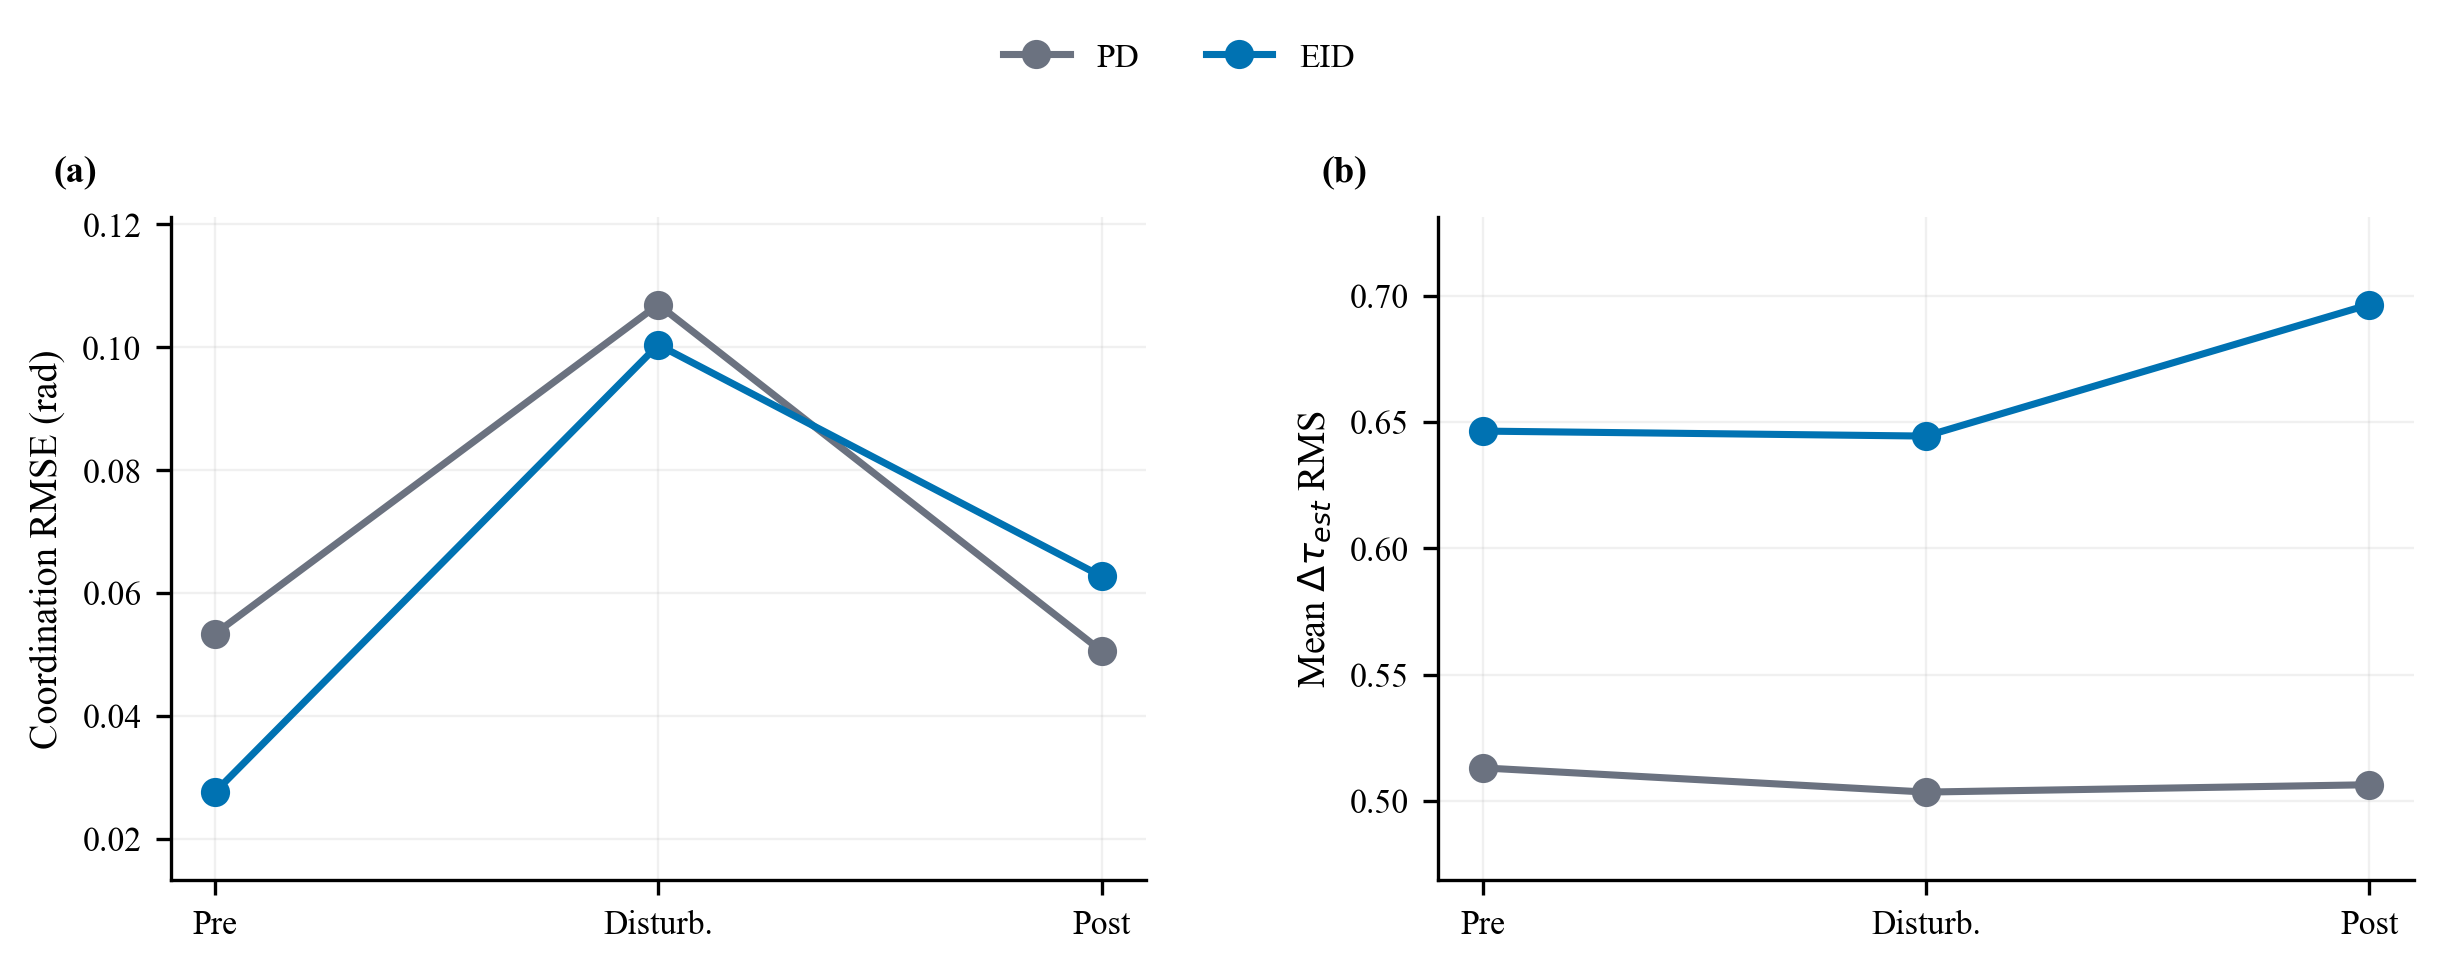
\includegraphics[keepaspectratio,alt={P2D 扰动窗口与恢复段统计}]{analysis_artifacts/bychen_answer/figures/bychen_p2d_window_recovery.png}}
\caption{P2D 扰动窗口与恢复段统计}
\end{figure}

\textbf{结论。} P2D 不能写成``EID 全部指标优于 PD''。准确表述应为：在当前软件输入端等效扰动下，EID 改善髋窗口 RMSE、协调窗口 RMSE 和峰值误差，但没有改善膝窗口 RMSE，并且增加 \texttt{tau\_est} RMS 与 \texttt{Delta\ tau\_est} RMS。

\subsection{\texorpdfstring{3.2 P4D：共同 \texttt{K\_o} 扫描}{3.2 P4D：共同 K\_o 扫描}}\label{p4dux5171ux540c-k_o-ux626bux63cf}

\begin{longtable}[]{@{}
  >{\raggedright\arraybackslash}p{(\linewidth - 16\tabcolsep) * \real{0.0857}}
  >{\raggedleft\arraybackslash}p{(\linewidth - 16\tabcolsep) * \real{0.1143}}
  >{\raggedleft\arraybackslash}p{(\linewidth - 16\tabcolsep) * \real{0.1143}}
  >{\raggedleft\arraybackslash}p{(\linewidth - 16\tabcolsep) * \real{0.1143}}
  >{\raggedleft\arraybackslash}p{(\linewidth - 16\tabcolsep) * \real{0.1143}}
  >{\raggedleft\arraybackslash}p{(\linewidth - 16\tabcolsep) * \real{0.1143}}
  >{\raggedleft\arraybackslash}p{(\linewidth - 16\tabcolsep) * \real{0.1143}}
  >{\raggedleft\arraybackslash}p{(\linewidth - 16\tabcolsep) * \real{0.1143}}
  >{\raggedleft\arraybackslash}p{(\linewidth - 16\tabcolsep) * \real{0.1143}}@{}}
\toprule\noalign{}
\begin{minipage}[b]{\linewidth}\raggedright
组别
\end{minipage} & \begin{minipage}[b]{\linewidth}\raggedleft
\texttt{K\_o} 缩放
\end{minipage} & \begin{minipage}[b]{\linewidth}\raggedleft
完整运行
\end{minipage} & \begin{minipage}[b]{\linewidth}\raggedleft
完整扰动窗口
\end{minipage} & \begin{minipage}[b]{\linewidth}\raggedleft
髋窗口 RMSE
\end{minipage} & \begin{minipage}[b]{\linewidth}\raggedleft
膝窗口 RMSE
\end{minipage} & \begin{minipage}[b]{\linewidth}\raggedleft
协调窗口 RMSE
\end{minipage} & \begin{minipage}[b]{\linewidth}\raggedleft
髋 \texttt{tau\_est} RMS
\end{minipage} & \begin{minipage}[b]{\linewidth}\raggedleft
膝 \texttt{tau\_est} RMS
\end{minipage} \\
\midrule\noalign{}
\endhead
\bottomrule\noalign{}
\endlastfoot
O0 & 0.00 & 0/3 & 0/3 & - & - & - & - & - \\
O1 & 0.25 & 2/3 & 3/3 & 0.0588 & 0.0755 & 0.1334 & 2.6362 & 2.5498 \\
O2 & 0.50 & 2/3 & 3/3 & 0.0529 & 0.0582 & 0.1101 & 2.5895 & 2.7183 \\
O3 & 0.75 & 2/3 & 3/3 & 0.0510 & 0.0532 & 0.1031 & 2.6378 & 2.9040 \\
O4 & 1.00 & 3/3 & 3/3 & 0.0499 & 0.0497 & 0.0984 & 2.6002 & 2.8164 \\
O5 & 1.25 & 3/3 & 3/3 & 0.0494 & 0.0485 & 0.0965 & 2.6647 & 2.8815 \\
\end{longtable}

\begin{figure}
\centering
\pandocbounded{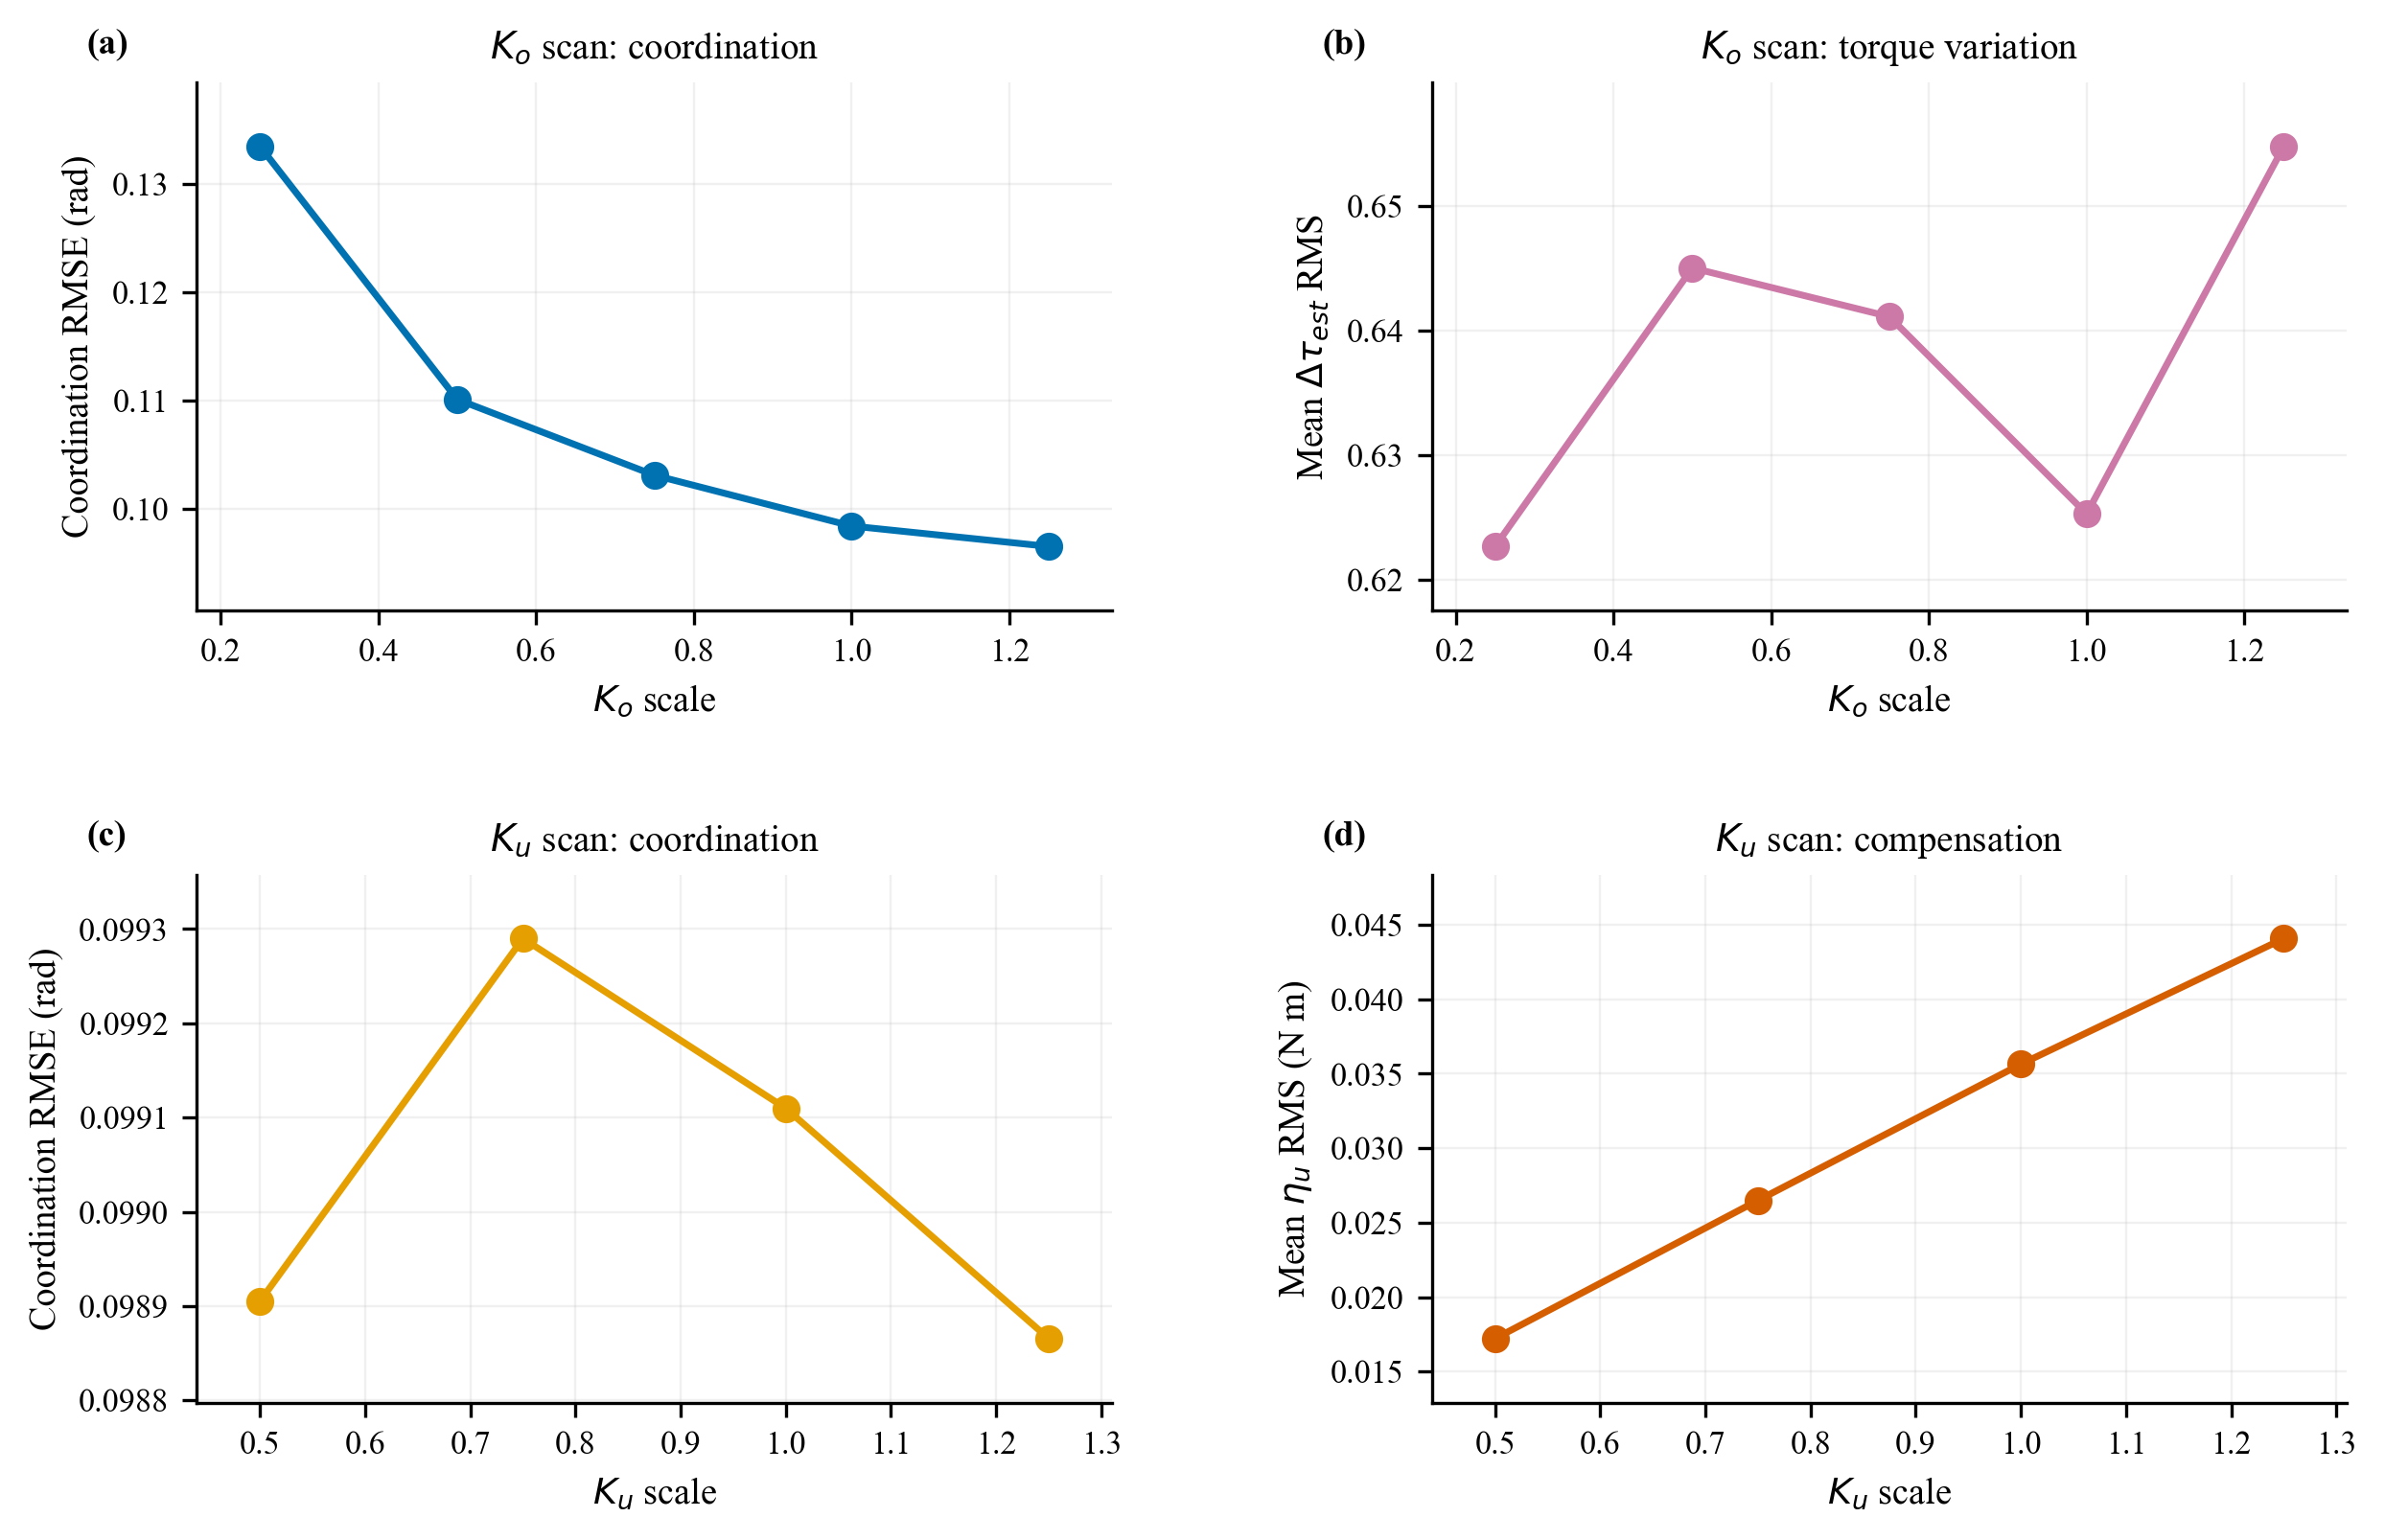
\includegraphics[keepaspectratio,alt={P4D 增益扫描}]{analysis_artifacts/bychen_answer/figures/bychen_p4d_gain_scans.png}}
\caption{P4D 增益扫描}
\end{figure}

\textbf{结论。} 当前 P4D 只说明共同增大 \texttt{K\_o} 时窗口 RMSE 下降，不能说明``髋增、膝减''的非对称调参已经成立。O4/O5 是本轮可运行的相邻高倍率候选，O5 的误差略低但力矩 RMS 略高。

\subsection{\texorpdfstring{3.3 P4D：\texttt{K\_u} 扫描}{3.3 P4D：K\_u 扫描}}\label{p4dk_u-ux626bux63cf}

\begin{longtable}[]{@{}
  >{\raggedright\arraybackslash}p{(\linewidth - 14\tabcolsep) * \real{0.0968}}
  >{\raggedleft\arraybackslash}p{(\linewidth - 14\tabcolsep) * \real{0.1290}}
  >{\raggedleft\arraybackslash}p{(\linewidth - 14\tabcolsep) * \real{0.1290}}
  >{\raggedleft\arraybackslash}p{(\linewidth - 14\tabcolsep) * \real{0.1290}}
  >{\raggedleft\arraybackslash}p{(\linewidth - 14\tabcolsep) * \real{0.1290}}
  >{\raggedleft\arraybackslash}p{(\linewidth - 14\tabcolsep) * \real{0.1290}}
  >{\raggedleft\arraybackslash}p{(\linewidth - 14\tabcolsep) * \real{0.1290}}
  >{\raggedleft\arraybackslash}p{(\linewidth - 14\tabcolsep) * \real{0.1290}}@{}}
\toprule\noalign{}
\begin{minipage}[b]{\linewidth}\raggedright
组别
\end{minipage} & \begin{minipage}[b]{\linewidth}\raggedleft
\texttt{K\_u} 缩放
\end{minipage} & \begin{minipage}[b]{\linewidth}\raggedleft
完整运行
\end{minipage} & \begin{minipage}[b]{\linewidth}\raggedleft
髋窗口 RMSE
\end{minipage} & \begin{minipage}[b]{\linewidth}\raggedleft
膝窗口 RMSE
\end{minipage} & \begin{minipage}[b]{\linewidth}\raggedleft
协调窗口 RMSE
\end{minipage} & \begin{minipage}[b]{\linewidth}\raggedleft
髋 \texttt{eta\_u} RMS
\end{minipage} & \begin{minipage}[b]{\linewidth}\raggedleft
膝 \texttt{eta\_u} RMS
\end{minipage} \\
\midrule\noalign{}
\endhead
\bottomrule\noalign{}
\endlastfoot
U1 & 0.50 & 3/3 & 0.0501 & 0.0499 & 0.0989 & 0.0107 & 0.0238 \\
U2 & 0.75 & 3/3 & 0.0505 & 0.0499 & 0.0993 & 0.0176 & 0.0354 \\
U3 & 1.00 & 3/3 & 0.0506 & 0.0499 & 0.0991 & 0.0240 & 0.0473 \\
U4 & 1.25 & 3/3 & 0.0504 & 0.0497 & 0.0989 & 0.0293 & 0.0589 \\
\end{longtable}

\textbf{结论。} 增大 \texttt{K\_u} 几乎不改善窗口 RMSE，只放大 \texttt{eta\_u} 活动量。低 \texttt{K\_u} 可作为保守补偿基线，但不能被写成解决真实力矩波动的主要手段。

\section{4. 参数定义与逐关节调参形式}\label{ux53c2ux6570ux5b9aux4e49ux4e0eux9010ux5173ux8282ux8c03ux53c2ux5f62ux5f0f}

后续分析使用观测器倍率 \texttt{s\_o} 表示 \texttt{K\_o} 的相对缩放：

\[
K_o=s_oK_o^{\rm nom},
\qquad
K_o^{\rm nom}=
\begin{bmatrix}
0.8 & 0\\
0 & 0.2
\end{bmatrix}.
\]

其中：

\begin{Shaded}
\begin{Highlighting}[]
\NormalTok{observer\_gain\_q  = 0.8}
\NormalTok{observer\_gain\_dq = 0.2}
\NormalTok{filter\_alpha     = 0.85}
\end{Highlighting}
\end{Shaded}

P4/P4D 的 O0--O5 对应：

\begin{longtable}[]{@{}lrrr@{}}
\toprule\noalign{}
组别 & \texttt{s\_o} & \texttt{observer\_gain\_q} & \texttt{observer\_gain\_dq} \\
\midrule\noalign{}
\endhead
\bottomrule\noalign{}
\endlastfoot
O0 & 0.00 & 0.0 & 0.00 \\
O1 & 0.25 & 0.2 & 0.05 \\
O2 & 0.50 & 0.4 & 0.10 \\
O3 & 0.75 & 0.6 & 0.15 \\
O4 & 1.00 & 0.8 & 0.20 \\
O5 & 1.25 & 1.0 & 0.25 \\
\end{longtable}

\texttt{K\_u} 缩放应写成输入补偿倍率 \texttt{s\_u}：

\[
K_u=s_uK_u^{\rm nom},
\qquad
K_u^{\rm nom}=
\begin{bmatrix}
12.0 & 1.0
\end{bmatrix}.
\]

U1--U4 分别对应 \texttt{s\_u=0.50,0.75,1.00,1.25}。

当前 \texttt{observer\_gain\_q=0.8}、\texttt{observer\_gain\_dq=0.2} 是前期实物调试形成的经验标称值，并在 P1/P2 EID、P4 O4 和 P4 U3 中作为可运行基准使用。原始设计过程尚未形成可追溯的极点或带宽依据，因此本轮只能把它定义为 \texttt{s\_o=1} 的扫描中心，用于相对敏感性分析，不能称为理论最优或跨关节统一最优。

逐关节调参使用：

\[
K_{o,j}=s_{o,j}K_{o,j}^{\rm nom},
\qquad
j\in\{\mathrm{hip},\mathrm{knee}\}.
\]

当前 P4D 相当于：

\[
s_{o,\mathrm{hip}}=s_{o,\mathrm{knee}}=s_o.
\]

下一轮需要允许：

\[
s_{o,\mathrm{hip}}\ne s_{o,\mathrm{knee}}.
\]

\section{5. 离线日志结果}\label{ux79bbux7ebfux65e5ux5fd7ux7ed3ux679c}

\subsection{5.1 P2D/P4D 频谱分析}\label{p2dp4d-ux9891ux8c31ux5206ux6790}

频谱分析用于判断力矩变化量增加集中在哪些频段，并区分正常跟踪频谱与扰动响应频谱。P2D 和 P4D 候选频谱结果如下。

P2D 频谱峰值：

\begin{longtable}[]{@{}lllrr@{}}
\toprule\noalign{}
方法 & 关节 & 信号 & 峰值频率 Hz & 峰值幅值 \\
\midrule\noalign{}
\endhead
\bottomrule\noalign{}
\endlastfoot
PD & Hip & \texttt{tau\_est} & 0.721 & 1.340 \\
PD & Hip & \texttt{delta\_tau\_est} & 75.859 & 0.0699 \\
EID & Hip & \texttt{tau\_est} & 2.161 & 1.507 \\
EID & Hip & \texttt{delta\_tau\_est} & 20.917 & 0.1471 \\
PD & Knee & \texttt{tau\_est} & 0.721 & 2.588 \\
PD & Knee & \texttt{delta\_tau\_est} & 90.308 & 0.0847 \\
EID & Knee & \texttt{tau\_est} & 0.720 & 2.481 \\
EID & Knee & \texttt{delta\_tau\_est} & 90.159 & 0.0953 \\
\end{longtable}

\begin{figure}
\centering
\pandocbounded{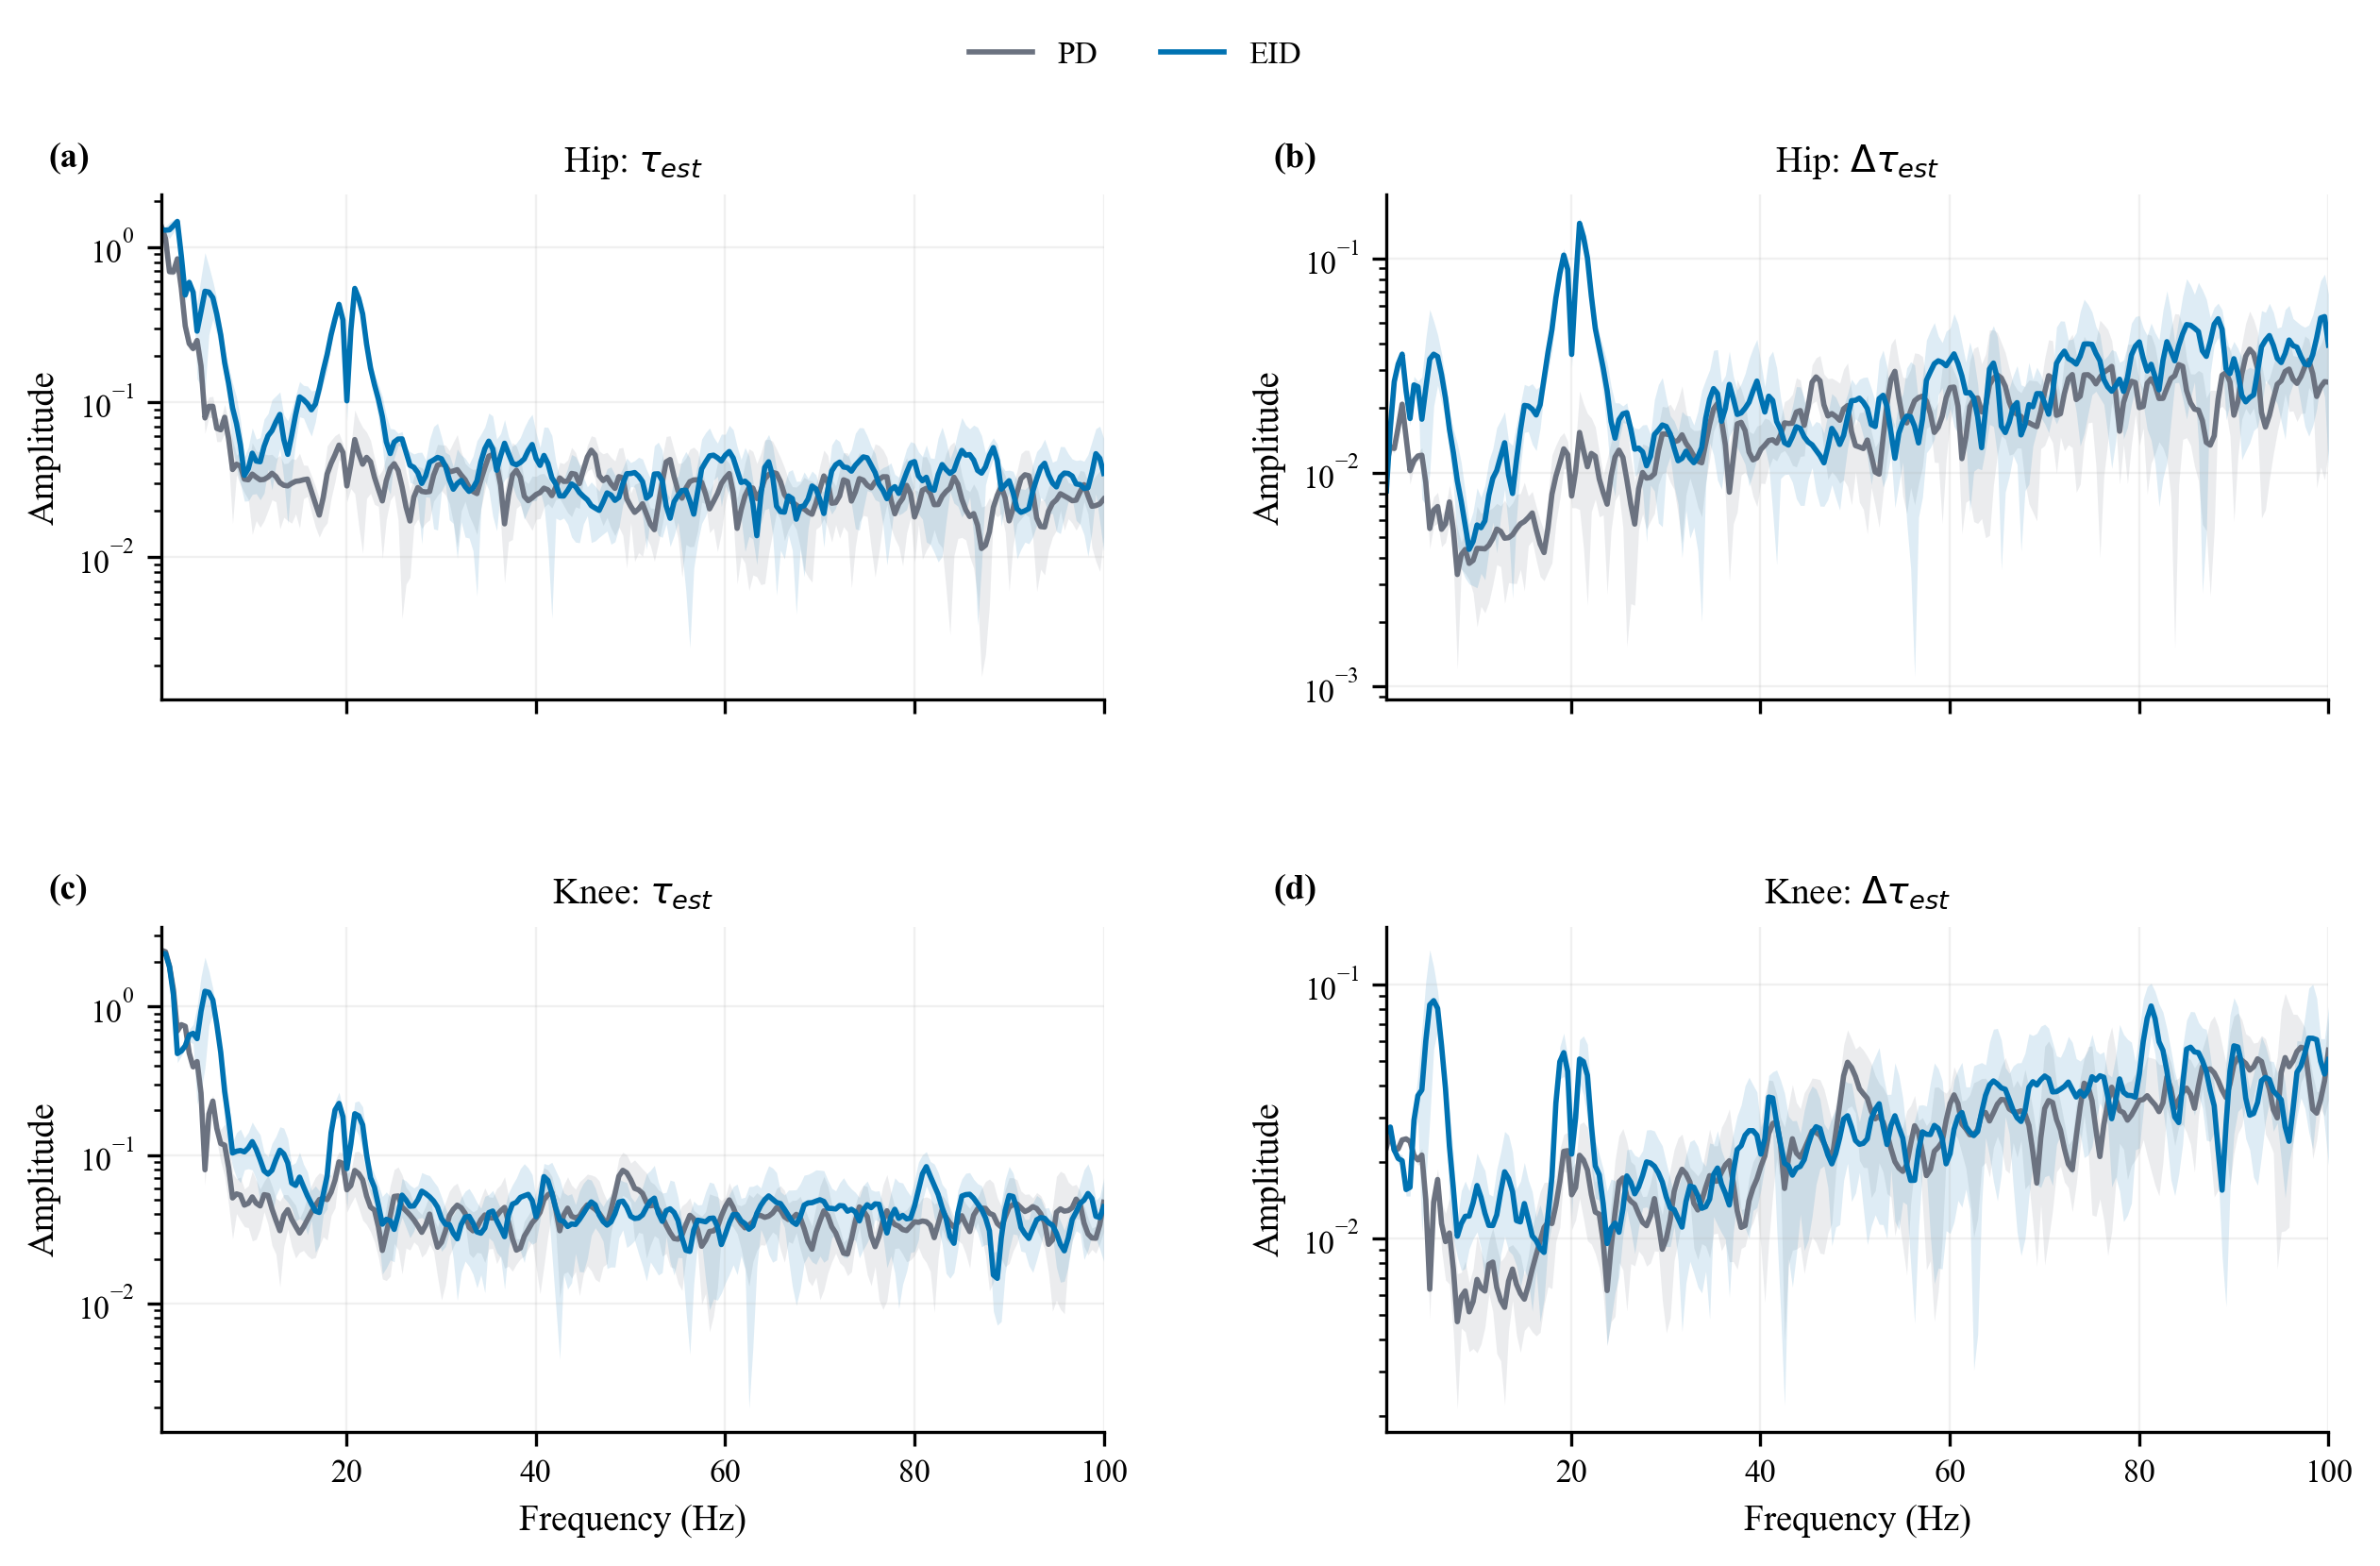
\includegraphics[keepaspectratio,alt={P2D 全重复频谱}]{analysis_artifacts/bychen_answer/figures/bychen_p2d_all_repeat_spectrum.png}}
\caption{P2D 全重复频谱}
\end{figure}

\begin{figure}
\centering
\pandocbounded{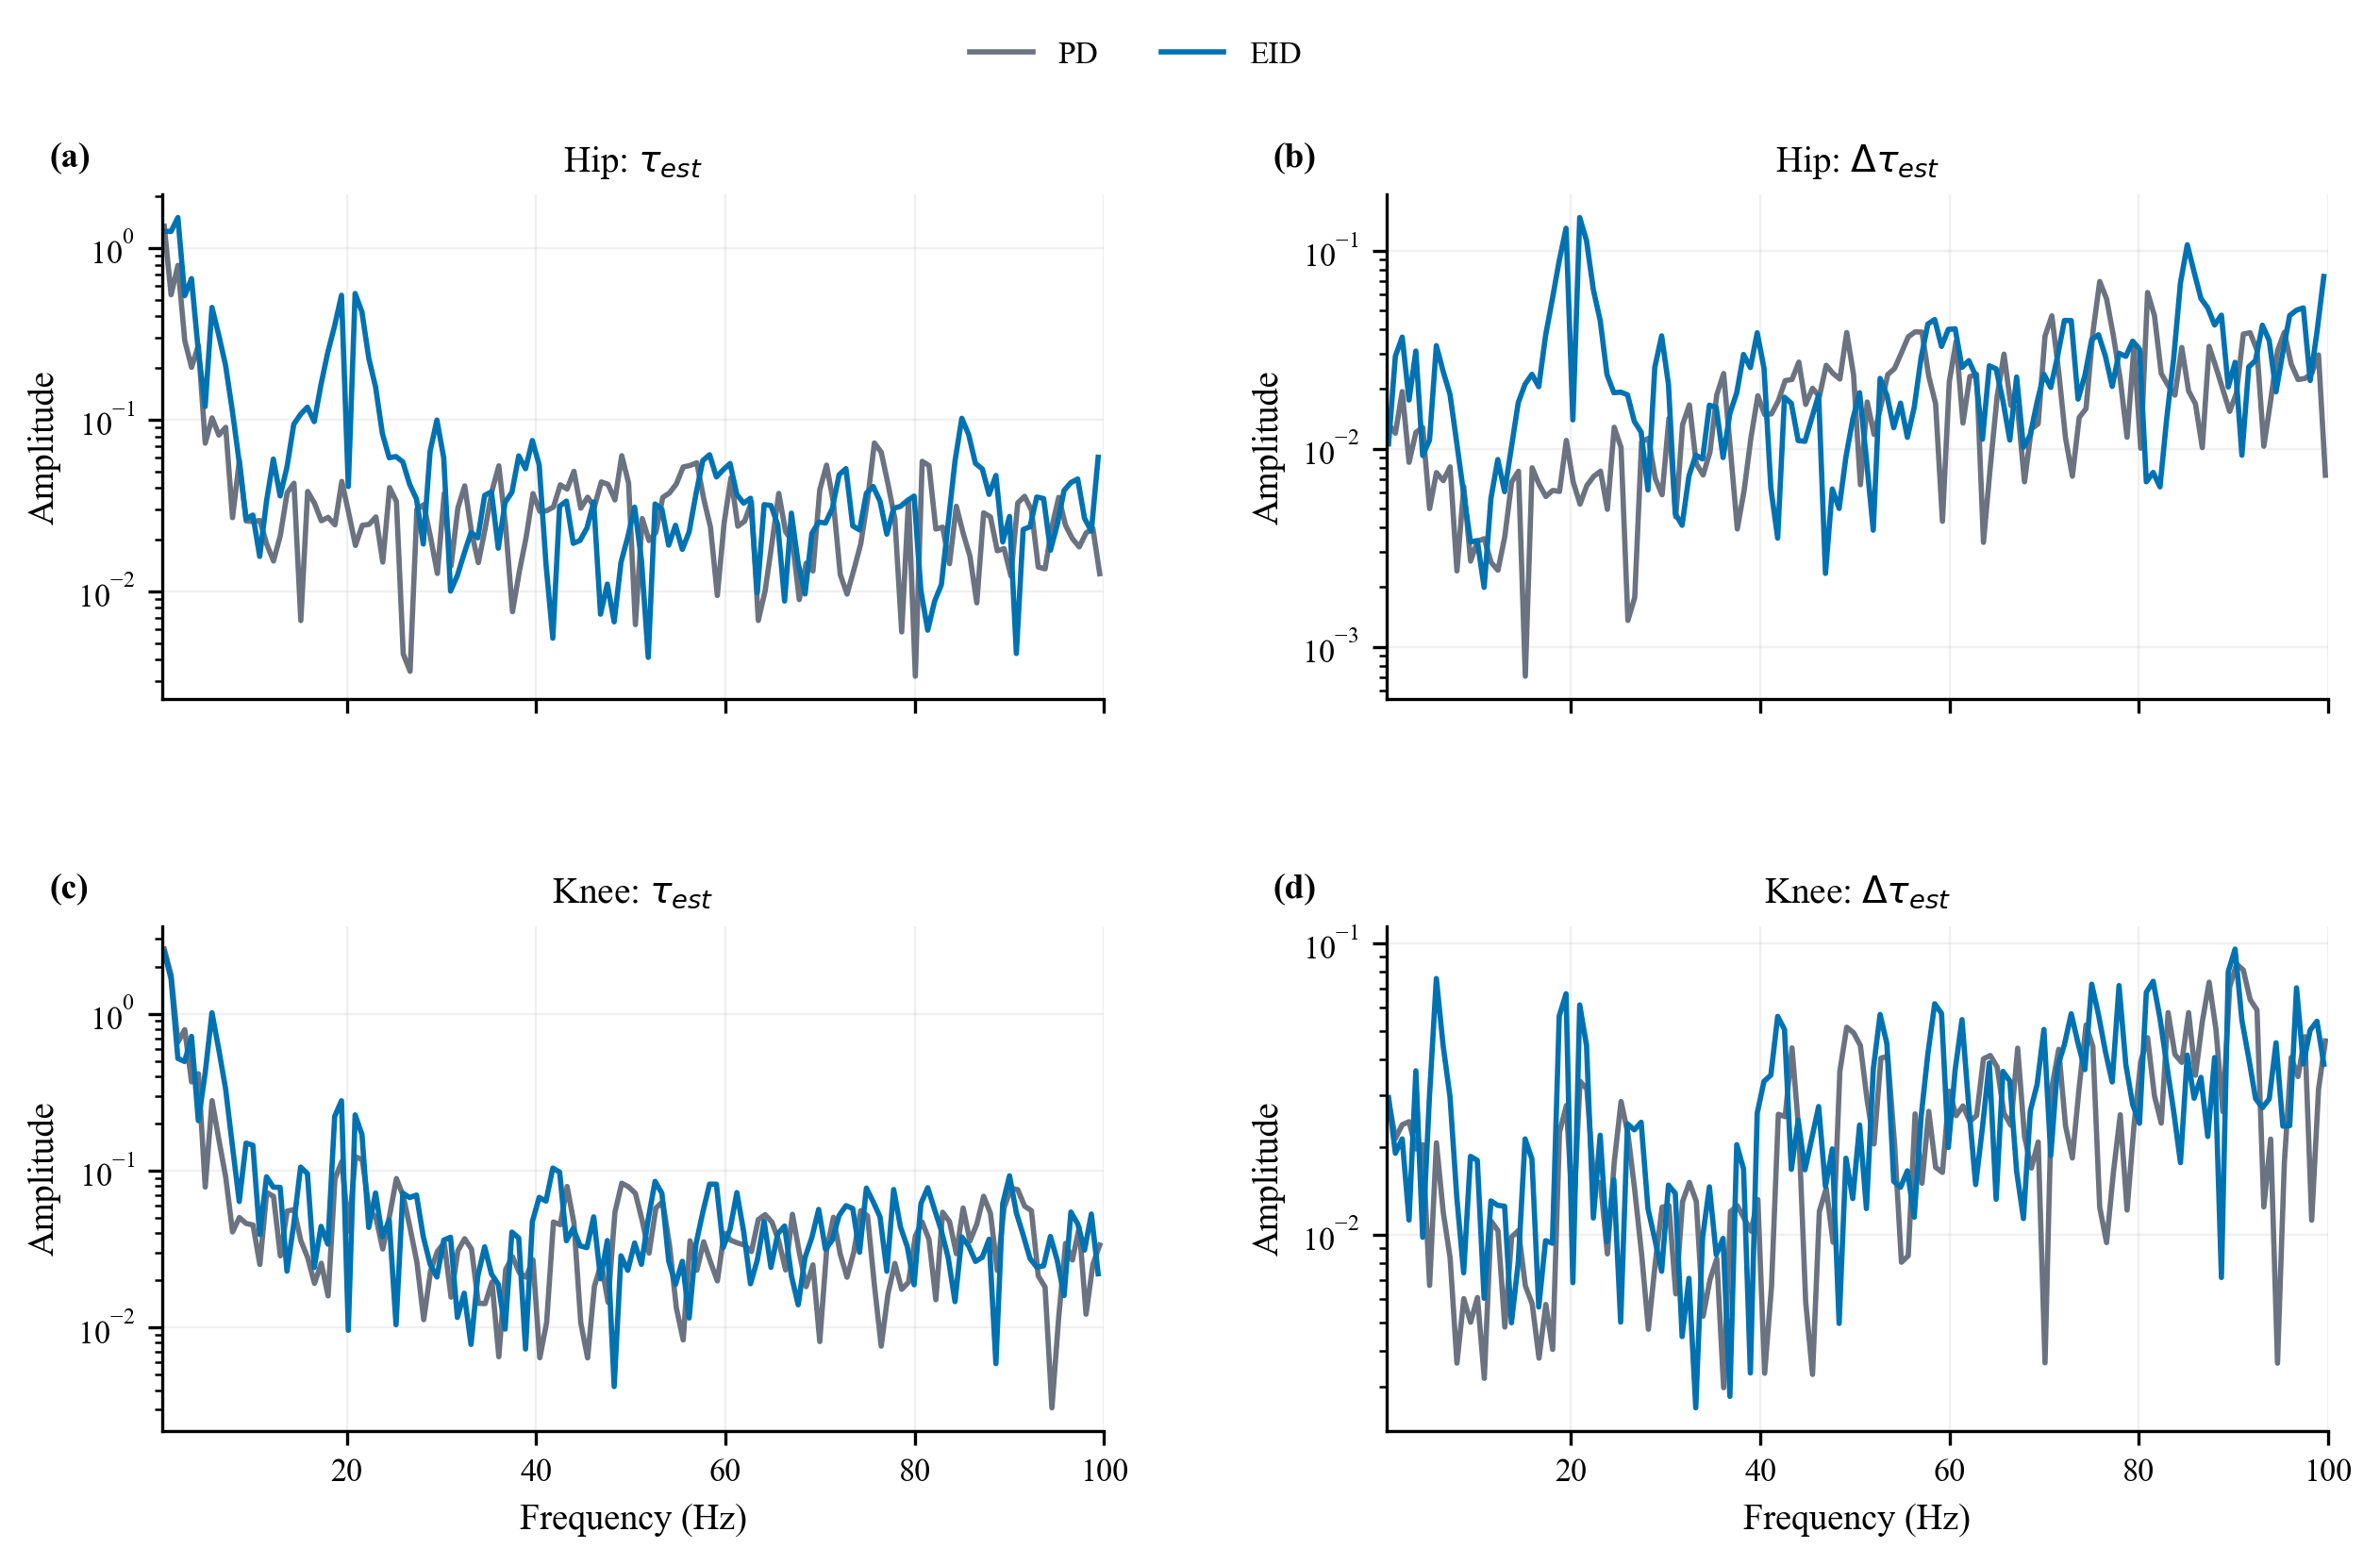
\includegraphics[keepaspectratio,alt={P2D 扰动窗口频谱}]{analysis_artifacts/bychen_answer/figures/bychen_p2d_disturbance_spectrum.png}}
\caption{P2D 扰动窗口频谱}
\end{figure}

P4D 候选频谱峰值：

\begin{longtable}[]{@{}lllrr@{}}
\toprule\noalign{}
候选 & 关节 & 信号 & 峰值频率 Hz & 平均峰值幅值 \\
\midrule\noalign{}
\endhead
\bottomrule\noalign{}
\endlastfoot
O4 & Coord & \texttt{coord\_error} & 0.500 & 0.0289 \\
O4 & Hip & \texttt{delta\_tau\_est} & 20.900 & 0.1503 \\
O4 & Knee & \texttt{delta\_tau\_est} & 89.592 & 0.0755 \\
O5 & Coord & \texttt{coord\_error} & 0.500 & 0.0265 \\
O5 & Hip & \texttt{eta\_u} & 15.904 & 0.0185 \\
O5 & Knee & \texttt{delta\_tau\_est} & 97.502 & 0.0791 \\
U1 & Coord & \texttt{coord\_error} & 0.500 & 0.0285 \\
U1 & Hip & \texttt{delta\_tau\_est} & 20.900 & 0.1619 \\
U1 & Knee & \texttt{eta\_u} & 0.500 & 0.00965 \\
U4 & Coord & \texttt{coord\_error} & 0.500 & 0.0270 \\
U4 & Hip & \texttt{delta\_tau\_est} & 20.900 & 0.1317 \\
\end{longtable}

\begin{figure}
\centering
\pandocbounded{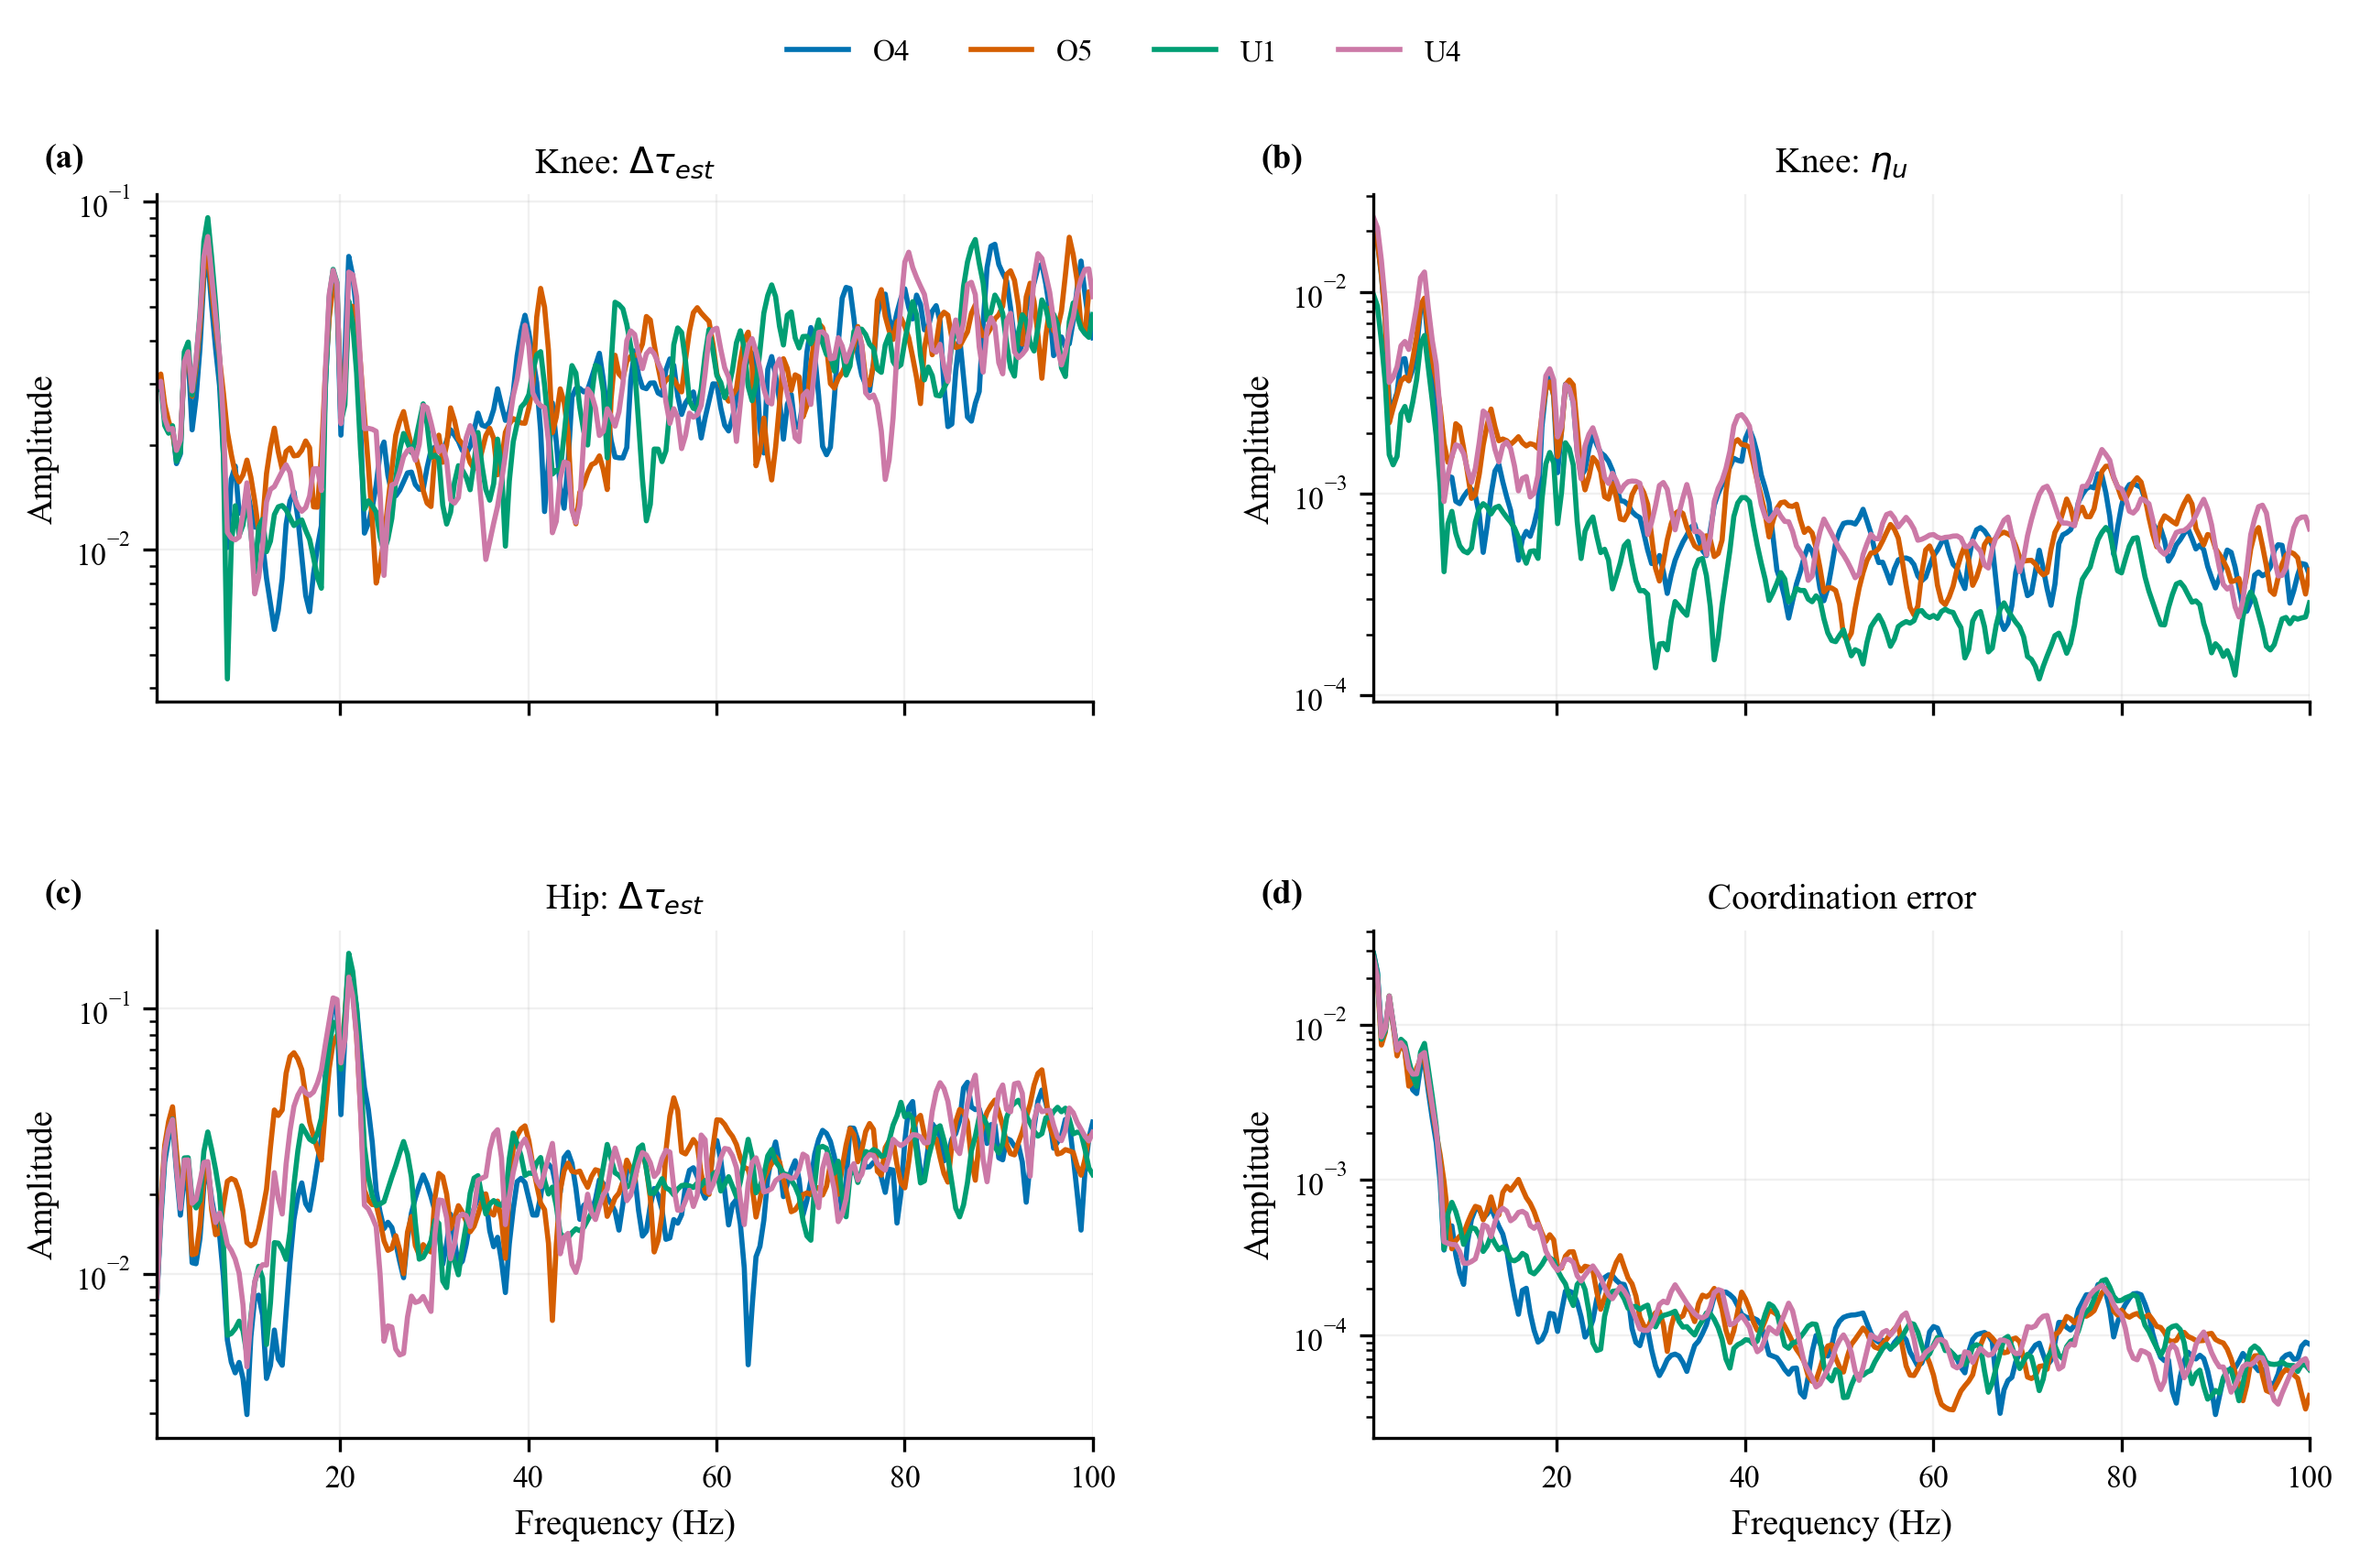
\includegraphics[keepaspectratio,alt={P4D 候选频谱}]{analysis_artifacts/bychen_answer/figures/bychen_p4d_candidate_spectrum.png}}
\caption{P4D 候选频谱}
\end{figure}

\textbf{结论。} O5 的协调误差频谱略低，但局部 \texttt{eta\_u} 和力矩高频活动更强；U1 是更保守的补偿基线。频谱结果支持``误差收益-力矩代价''共同评价，而不是只按 RMSE 排名。

\subsection{5.2 恢复段统计}\label{ux6062ux590dux6bb5ux7edfux8ba1}

恢复段统计用于回答扰动撤除后是否出现反冲或慢回稳。

\begin{figure}
\centering
\pandocbounded{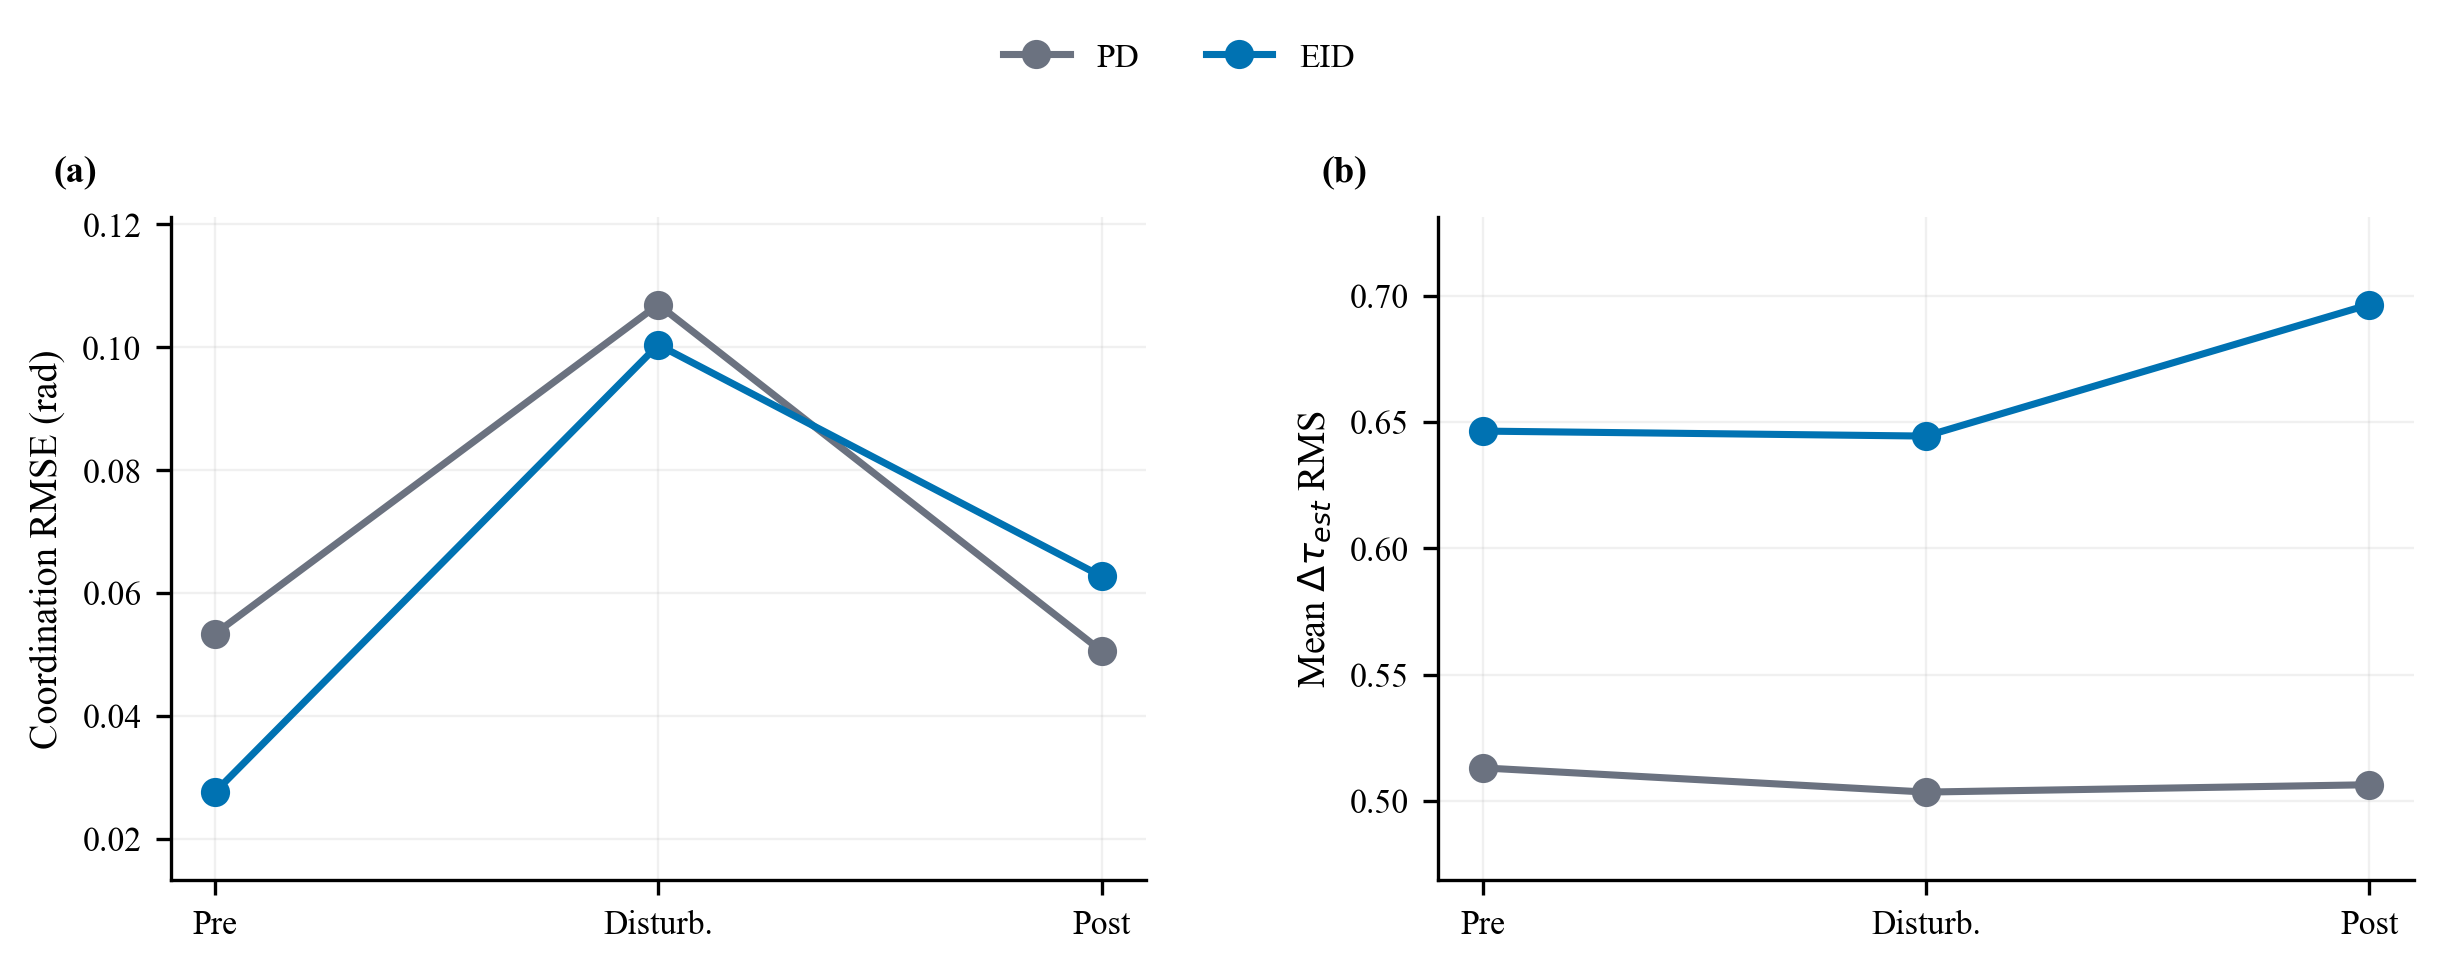
\includegraphics[keepaspectratio,alt={P2D 窗口与恢复段统计}]{analysis_artifacts/bychen_answer/figures/bychen_p2d_window_recovery.png}}
\caption{P2D 窗口与恢复段统计}
\end{figure}

\begin{figure}
\centering
\pandocbounded{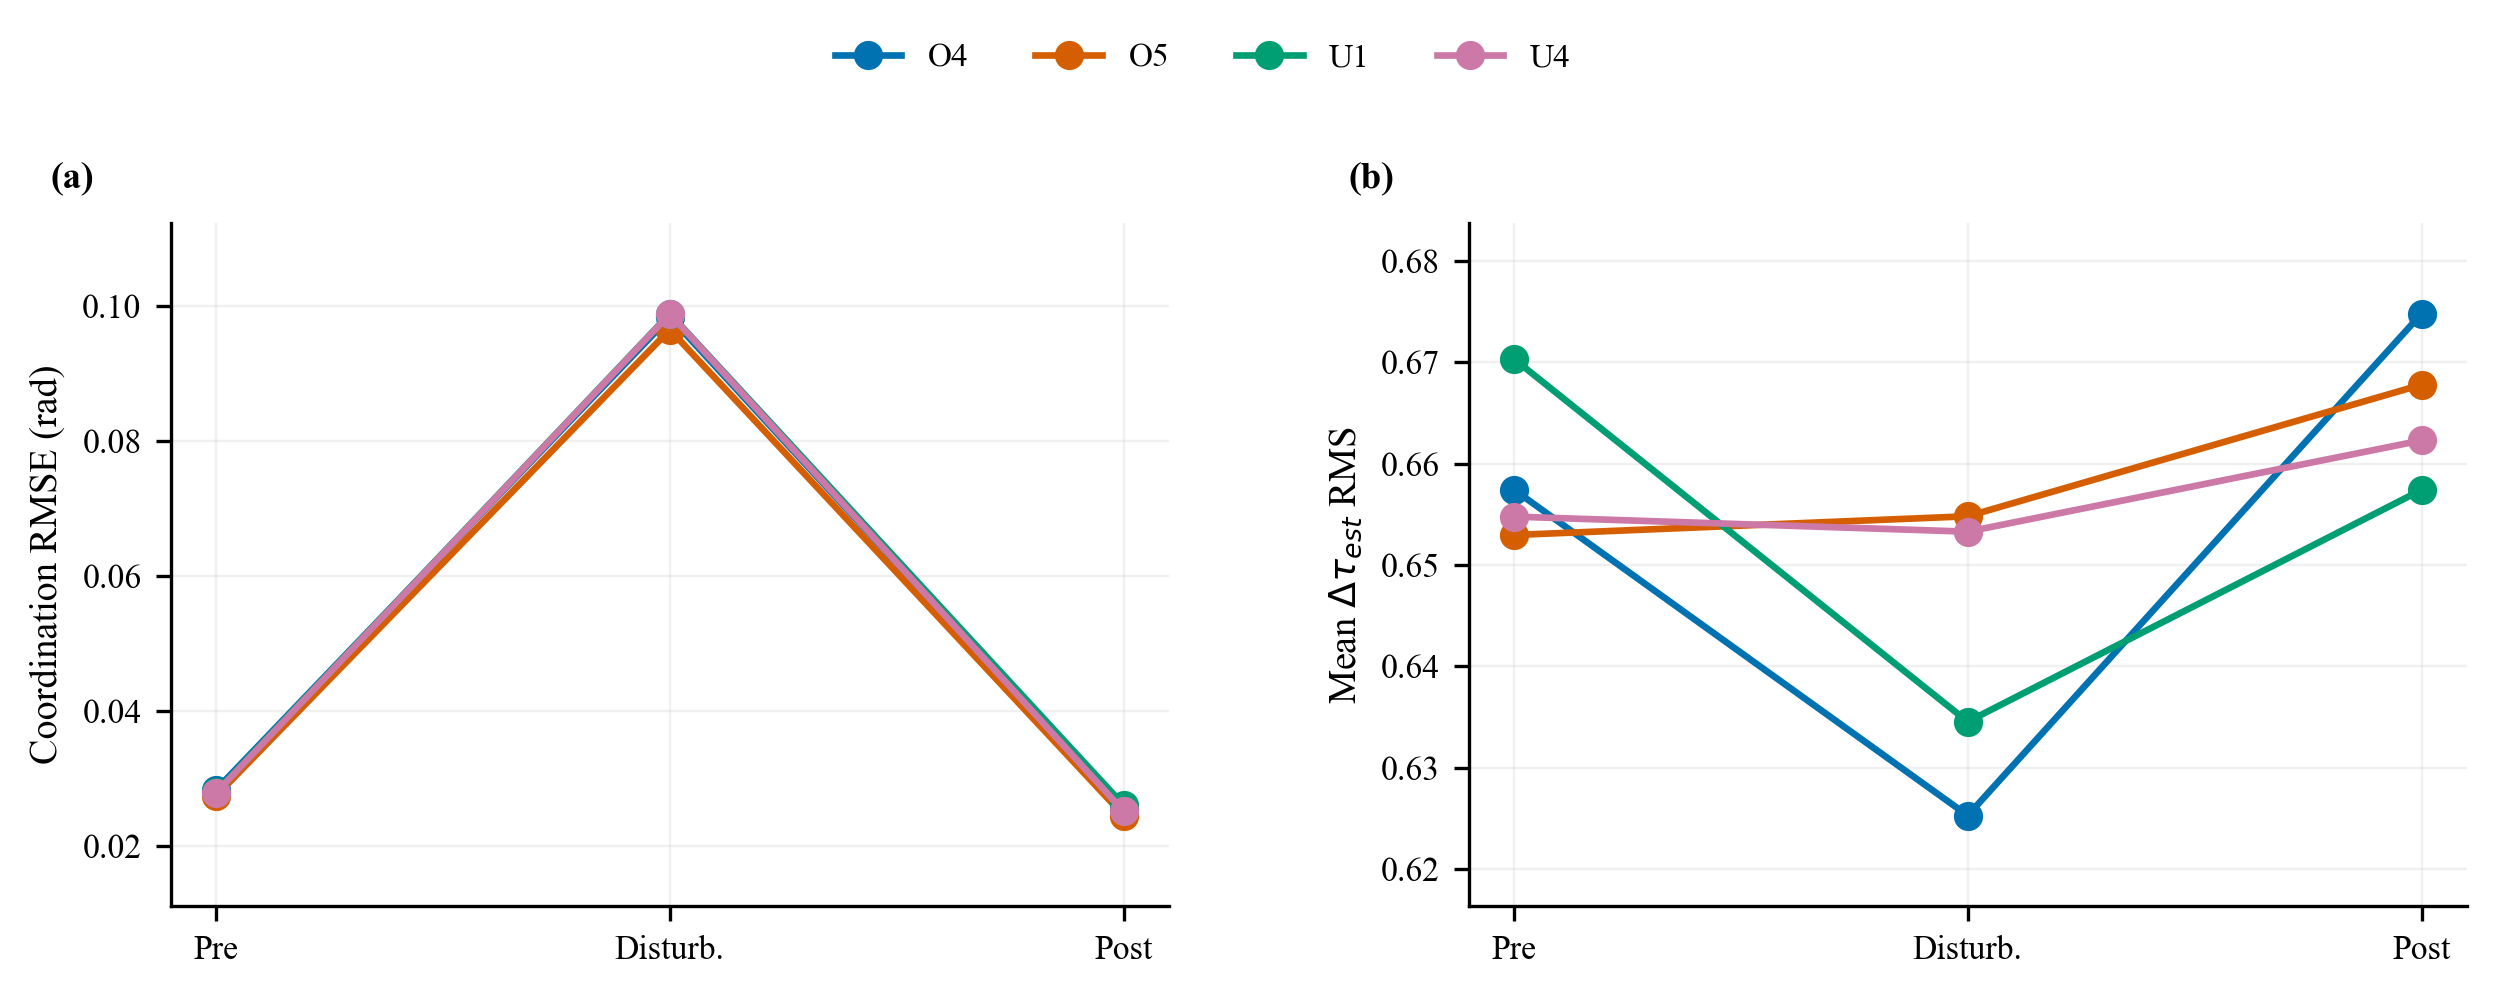
\includegraphics[keepaspectratio,alt={P4D 候选窗口统计}]{analysis_artifacts/bychen_answer/figures/bychen_p4d_candidate_windows.png}}
\caption{P4D 候选窗口统计}
\end{figure}

\textbf{结论。} 恢复段仍基于软件输入端等效扰动，不等价于真实外部接触力；但它已经可以用于筛掉扰动窗口表现好、恢复阶段反冲大的候选。

\subsection{\texorpdfstring{5.3 \texttt{eta\_u} 与软件扰动对齐}{5.3 eta\_u 与软件扰动对齐}}\label{eta_u-ux4e0eux8f6fux4ef6ux6270ux52a8ux5bf9ux9f50}

\texttt{eta\_u} 与已知软件扰动的 RMS 比值很小，且相关性并不支持把 \texttt{eta\_u} 简单解释为真实输入扰动估计。

\begin{longtable}[]{@{}llrrr@{}}
\toprule\noalign{}
条件 & 关节 & \texttt{eta\_u} / 扰动 RMS 比值 & 同采样相关 & 最大相关绝对值 \\
\midrule\noalign{}
\endhead
\bottomrule\noalign{}
\endlastfoot
P2D & Hip & 0.00394 & -0.312 & 0.319 \\
P2D & Knee & 0.01296 & -0.610 & 0.623 \\
O4 & Hip & 0.00357 & -0.341 & 0.356 \\
O4 & Knee & 0.01297 & -0.649 & 0.657 \\
O5 & Hip & 0.00540 & -0.182 & 0.196 \\
O5 & Knee & 0.01298 & -0.623 & 0.635 \\
U1 & Hip & 0.00196 & -0.296 & 0.308 \\
U1 & Knee & 0.00656 & -0.631 & 0.643 \\
\end{longtable}

\begin{figure}
\centering
\pandocbounded{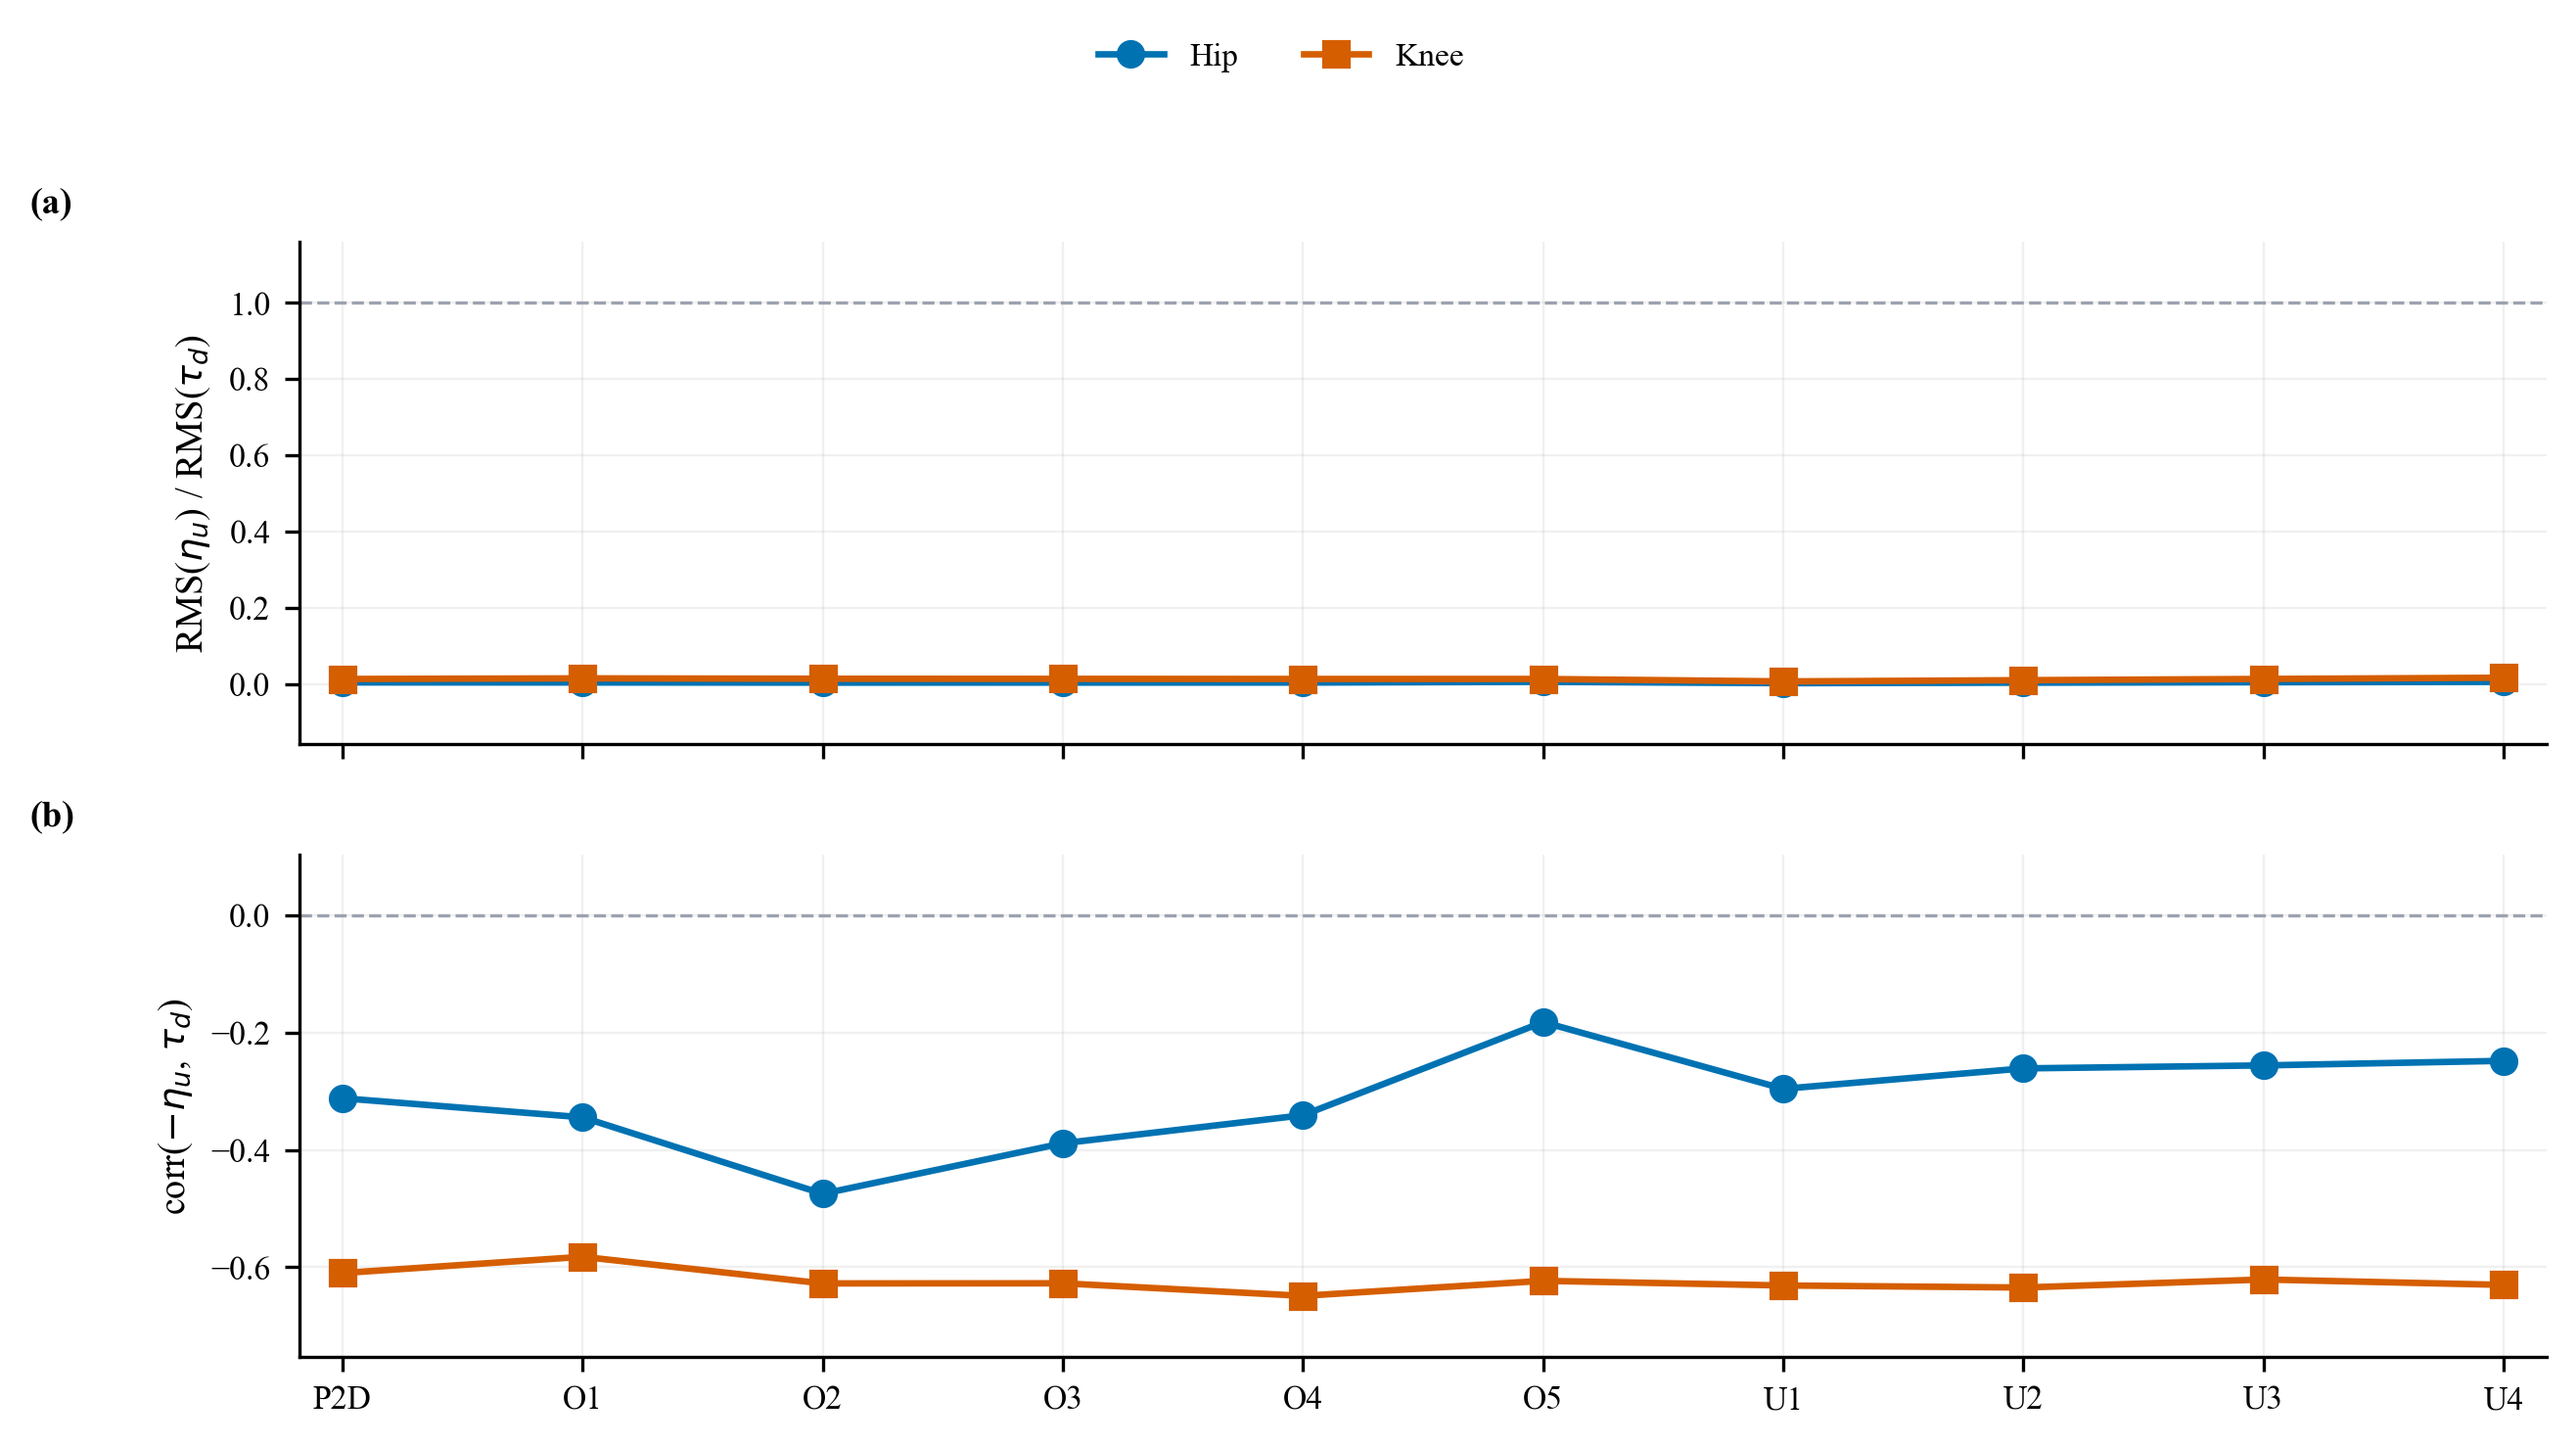
\includegraphics[keepaspectratio,alt={eta\_u 与软件扰动对齐}]{analysis_artifacts/bychen_answer/figures/bychen_eta_disturbance_alignment.png}}
\caption{eta\_u 与软件扰动对齐}
\end{figure}

\textbf{结论。} \texttt{eta\_u} 的幅值远小于已知软件扰动，且相关性不支持把它直接写成``扰动力矩估计''。这解释了为什么提高 \texttt{K\_u} 主要增加内部补偿活动，而不是明显降低窗口 RMSE。

\subsection{5.4 力矩项分解}\label{ux529bux77e9ux9879ux5206ux89e3}

P2D 和 P4D 的力矩项分解显示，反馈项 RMS 远大于 \texttt{eta\_u} 输入补偿项。

\begin{longtable}[]{@{}
  >{\raggedright\arraybackslash}p{(\linewidth - 12\tabcolsep) * \real{0.1154}}
  >{\raggedright\arraybackslash}p{(\linewidth - 12\tabcolsep) * \real{0.1154}}
  >{\raggedleft\arraybackslash}p{(\linewidth - 12\tabcolsep) * \real{0.1538}}
  >{\raggedleft\arraybackslash}p{(\linewidth - 12\tabcolsep) * \real{0.1538}}
  >{\raggedleft\arraybackslash}p{(\linewidth - 12\tabcolsep) * \real{0.1538}}
  >{\raggedleft\arraybackslash}p{(\linewidth - 12\tabcolsep) * \real{0.1538}}
  >{\raggedleft\arraybackslash}p{(\linewidth - 12\tabcolsep) * \real{0.1538}}@{}}
\toprule\noalign{}
\begin{minipage}[b]{\linewidth}\raggedright
条件
\end{minipage} & \begin{minipage}[b]{\linewidth}\raggedright
关节
\end{minipage} & \begin{minipage}[b]{\linewidth}\raggedleft
\texttt{u\_star} RMS
\end{minipage} & \begin{minipage}[b]{\linewidth}\raggedleft
\texttt{u\_feedback} RMS
\end{minipage} & \begin{minipage}[b]{\linewidth}\raggedleft
\texttt{u\_eid\_comp} RMS
\end{minipage} & \begin{minipage}[b]{\linewidth}\raggedleft
\texttt{tau\_est} RMS
\end{minipage} & \begin{minipage}[b]{\linewidth}\raggedleft
扰动 RMS
\end{minipage} \\
\midrule\noalign{}
\endhead
\bottomrule\noalign{}
\endlastfoot
P2D & Hip & 2.581 & 6.001 & 0.0214 & 2.803 & 5.438 \\
P2D & Knee & 1.124 & 5.327 & 0.0470 & 2.795 & 3.626 \\
O4 & Hip & 2.580 & 5.773 & 0.0194 & 2.600 & 5.439 \\
O4 & Knee & 1.124 & 5.200 & 0.0470 & 2.816 & 3.626 \\
O5 & Hip & 2.579 & 5.830 & 0.0294 & 2.665 & 5.439 \\
O5 & Knee & 1.124 & 5.301 & 0.0471 & 2.881 & 3.626 \\
U1 & Hip & 2.580 & 5.811 & 0.0107 & 2.642 & 5.439 \\
U1 & Knee & 1.124 & 5.242 & 0.0238 & 2.826 & 3.626 \\
\end{longtable}

\begin{figure}
\centering
\pandocbounded{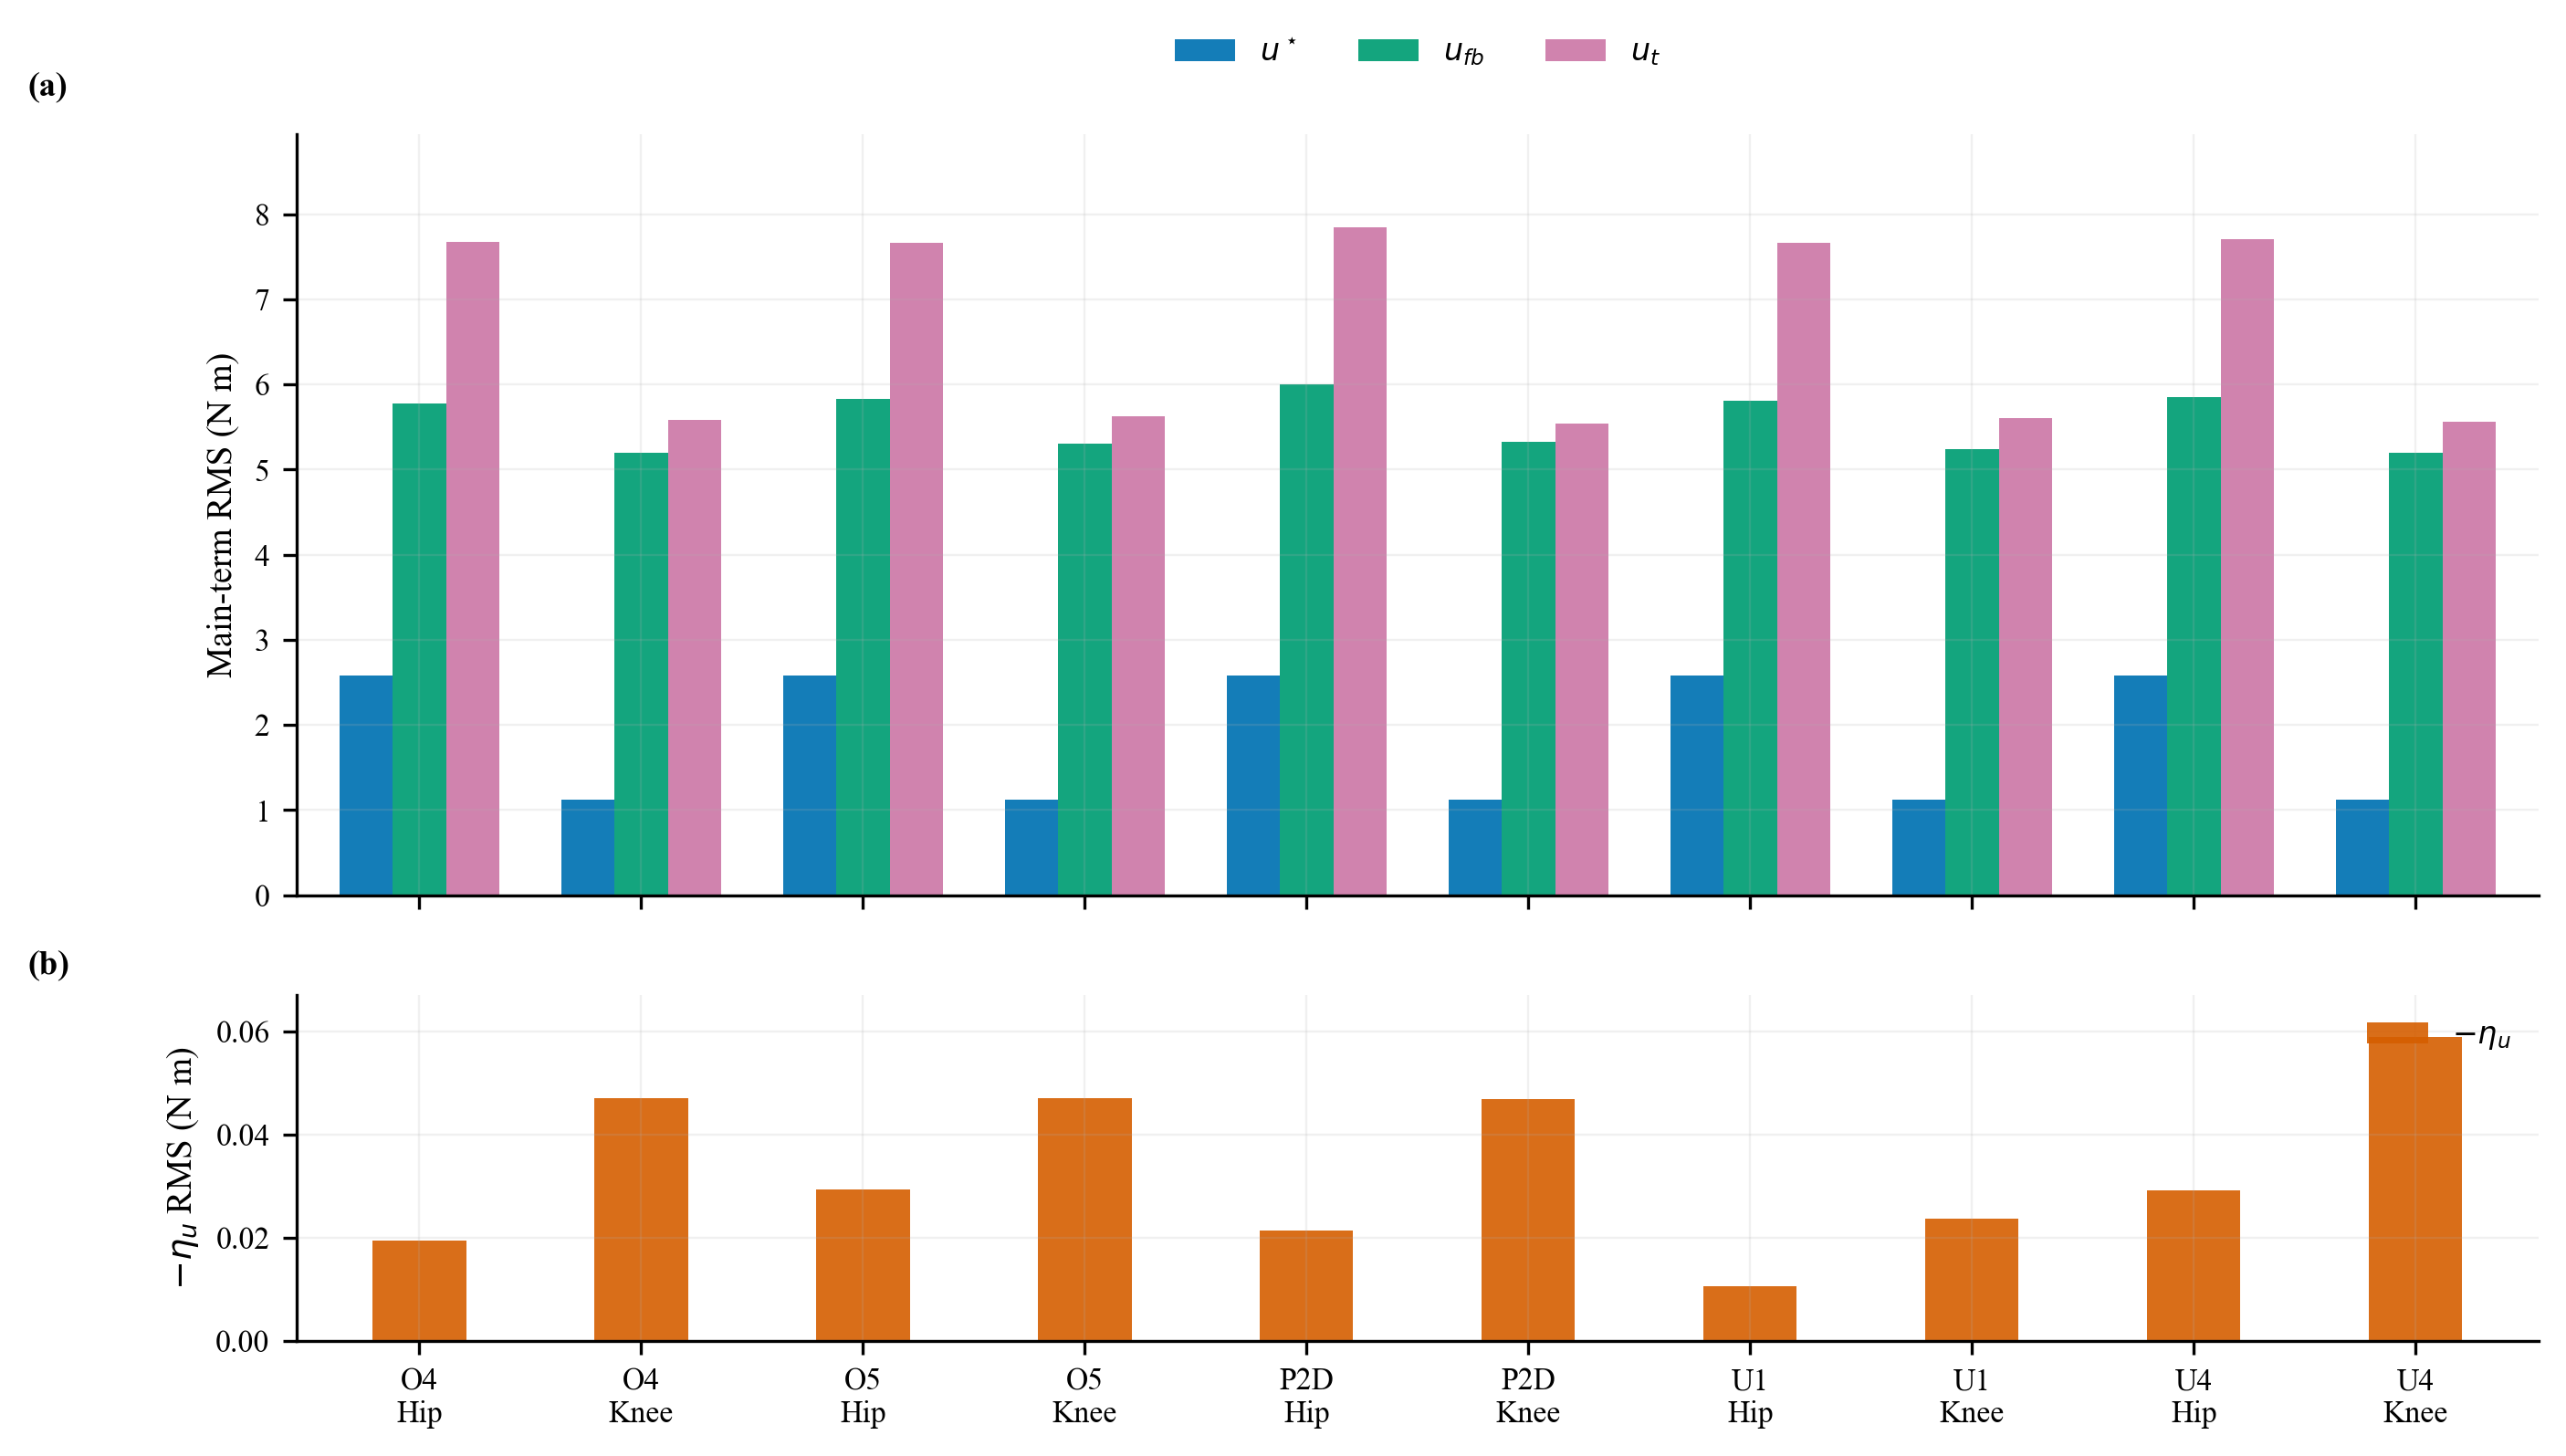
\includegraphics[keepaspectratio,alt={力矩项分解}]{analysis_artifacts/bychen_answer/figures/bychen_force_decomposition.png}}
\caption{力矩项分解}
\end{figure}

\textbf{结论。} 当前 EID 的可调性主要来自观测器残差、反馈中心构造和残差定义；\texttt{K\_u} 更适合作为内部补偿活动与力矩代价的约束通道。

\subsection{5.5 多目标 Pareto 与权重敏感性}\label{ux591aux76eeux6807-pareto-ux4e0eux6743ux91cdux654fux611fux6027}

单一权重不应决定参数推荐。现有 Pareto 点如下：

\begin{longtable}[]{@{}
  >{\raggedright\arraybackslash}p{(\linewidth - 18\tabcolsep) * \real{0.0833}}
  >{\raggedright\arraybackslash}p{(\linewidth - 18\tabcolsep) * \real{0.0833}}
  >{\raggedright\arraybackslash}p{(\linewidth - 18\tabcolsep) * \real{0.0833}}
  >{\raggedright\arraybackslash}p{(\linewidth - 18\tabcolsep) * \real{0.0833}}
  >{\raggedleft\arraybackslash}p{(\linewidth - 18\tabcolsep) * \real{0.1111}}
  >{\raggedleft\arraybackslash}p{(\linewidth - 18\tabcolsep) * \real{0.1111}}
  >{\raggedleft\arraybackslash}p{(\linewidth - 18\tabcolsep) * \real{0.1111}}
  >{\raggedleft\arraybackslash}p{(\linewidth - 18\tabcolsep) * \real{0.1111}}
  >{\raggedleft\arraybackslash}p{(\linewidth - 18\tabcolsep) * \real{0.1111}}
  >{\raggedleft\arraybackslash}p{(\linewidth - 18\tabcolsep) * \real{0.1111}}@{}}
\toprule\noalign{}
\begin{minipage}[b]{\linewidth}\raggedright
条件
\end{minipage} & \begin{minipage}[b]{\linewidth}\raggedright
方法
\end{minipage} & \begin{minipage}[b]{\linewidth}\raggedright
扫描
\end{minipage} & \begin{minipage}[b]{\linewidth}\raggedright
组别
\end{minipage} & \begin{minipage}[b]{\linewidth}\raggedleft
运行数
\end{minipage} & \begin{minipage}[b]{\linewidth}\raggedleft
完整窗口
\end{minipage} & \begin{minipage}[b]{\linewidth}\raggedleft
协调 RMSE
\end{minipage} & \begin{minipage}[b]{\linewidth}\raggedleft
平均 \texttt{Delta\ tau\_est} RMS
\end{minipage} & \begin{minipage}[b]{\linewidth}\raggedleft
平均 \texttt{tau\_est} RMS
\end{minipage} & \begin{minipage}[b]{\linewidth}\raggedleft
平均 \texttt{eta\_u} RMS
\end{minipage} \\
\midrule\noalign{}
\endhead
\bottomrule\noalign{}
\endlastfoot
P2D & EID & - & - & 5 & 5 & 0.1004 & 0.6444 & 2.7992 & 0.0342 \\
P2D & PD & - & - & 5 & 5 & 0.1069 & 0.5035 & 2.2386 & 0 \\
P4D & EID & ko & O4 & 3 & 3 & 0.0984 & 0.6253 & 2.7083 & 0.0332 \\
P4D & EID & ko & O5 & 3 & 3 & 0.0965 & 0.6548 & 2.7731 & 0.0382 \\
P4D & EID & ku & U1 & 3 & 3 & 0.0989 & 0.6345 & 2.7341 & 0.0172 \\
P4D & EID & ku & U4 & 3 & 3 & 0.0989 & 0.6533 & 2.7315 & 0.0441 \\
\end{longtable}

\begin{figure}
\centering
\pandocbounded{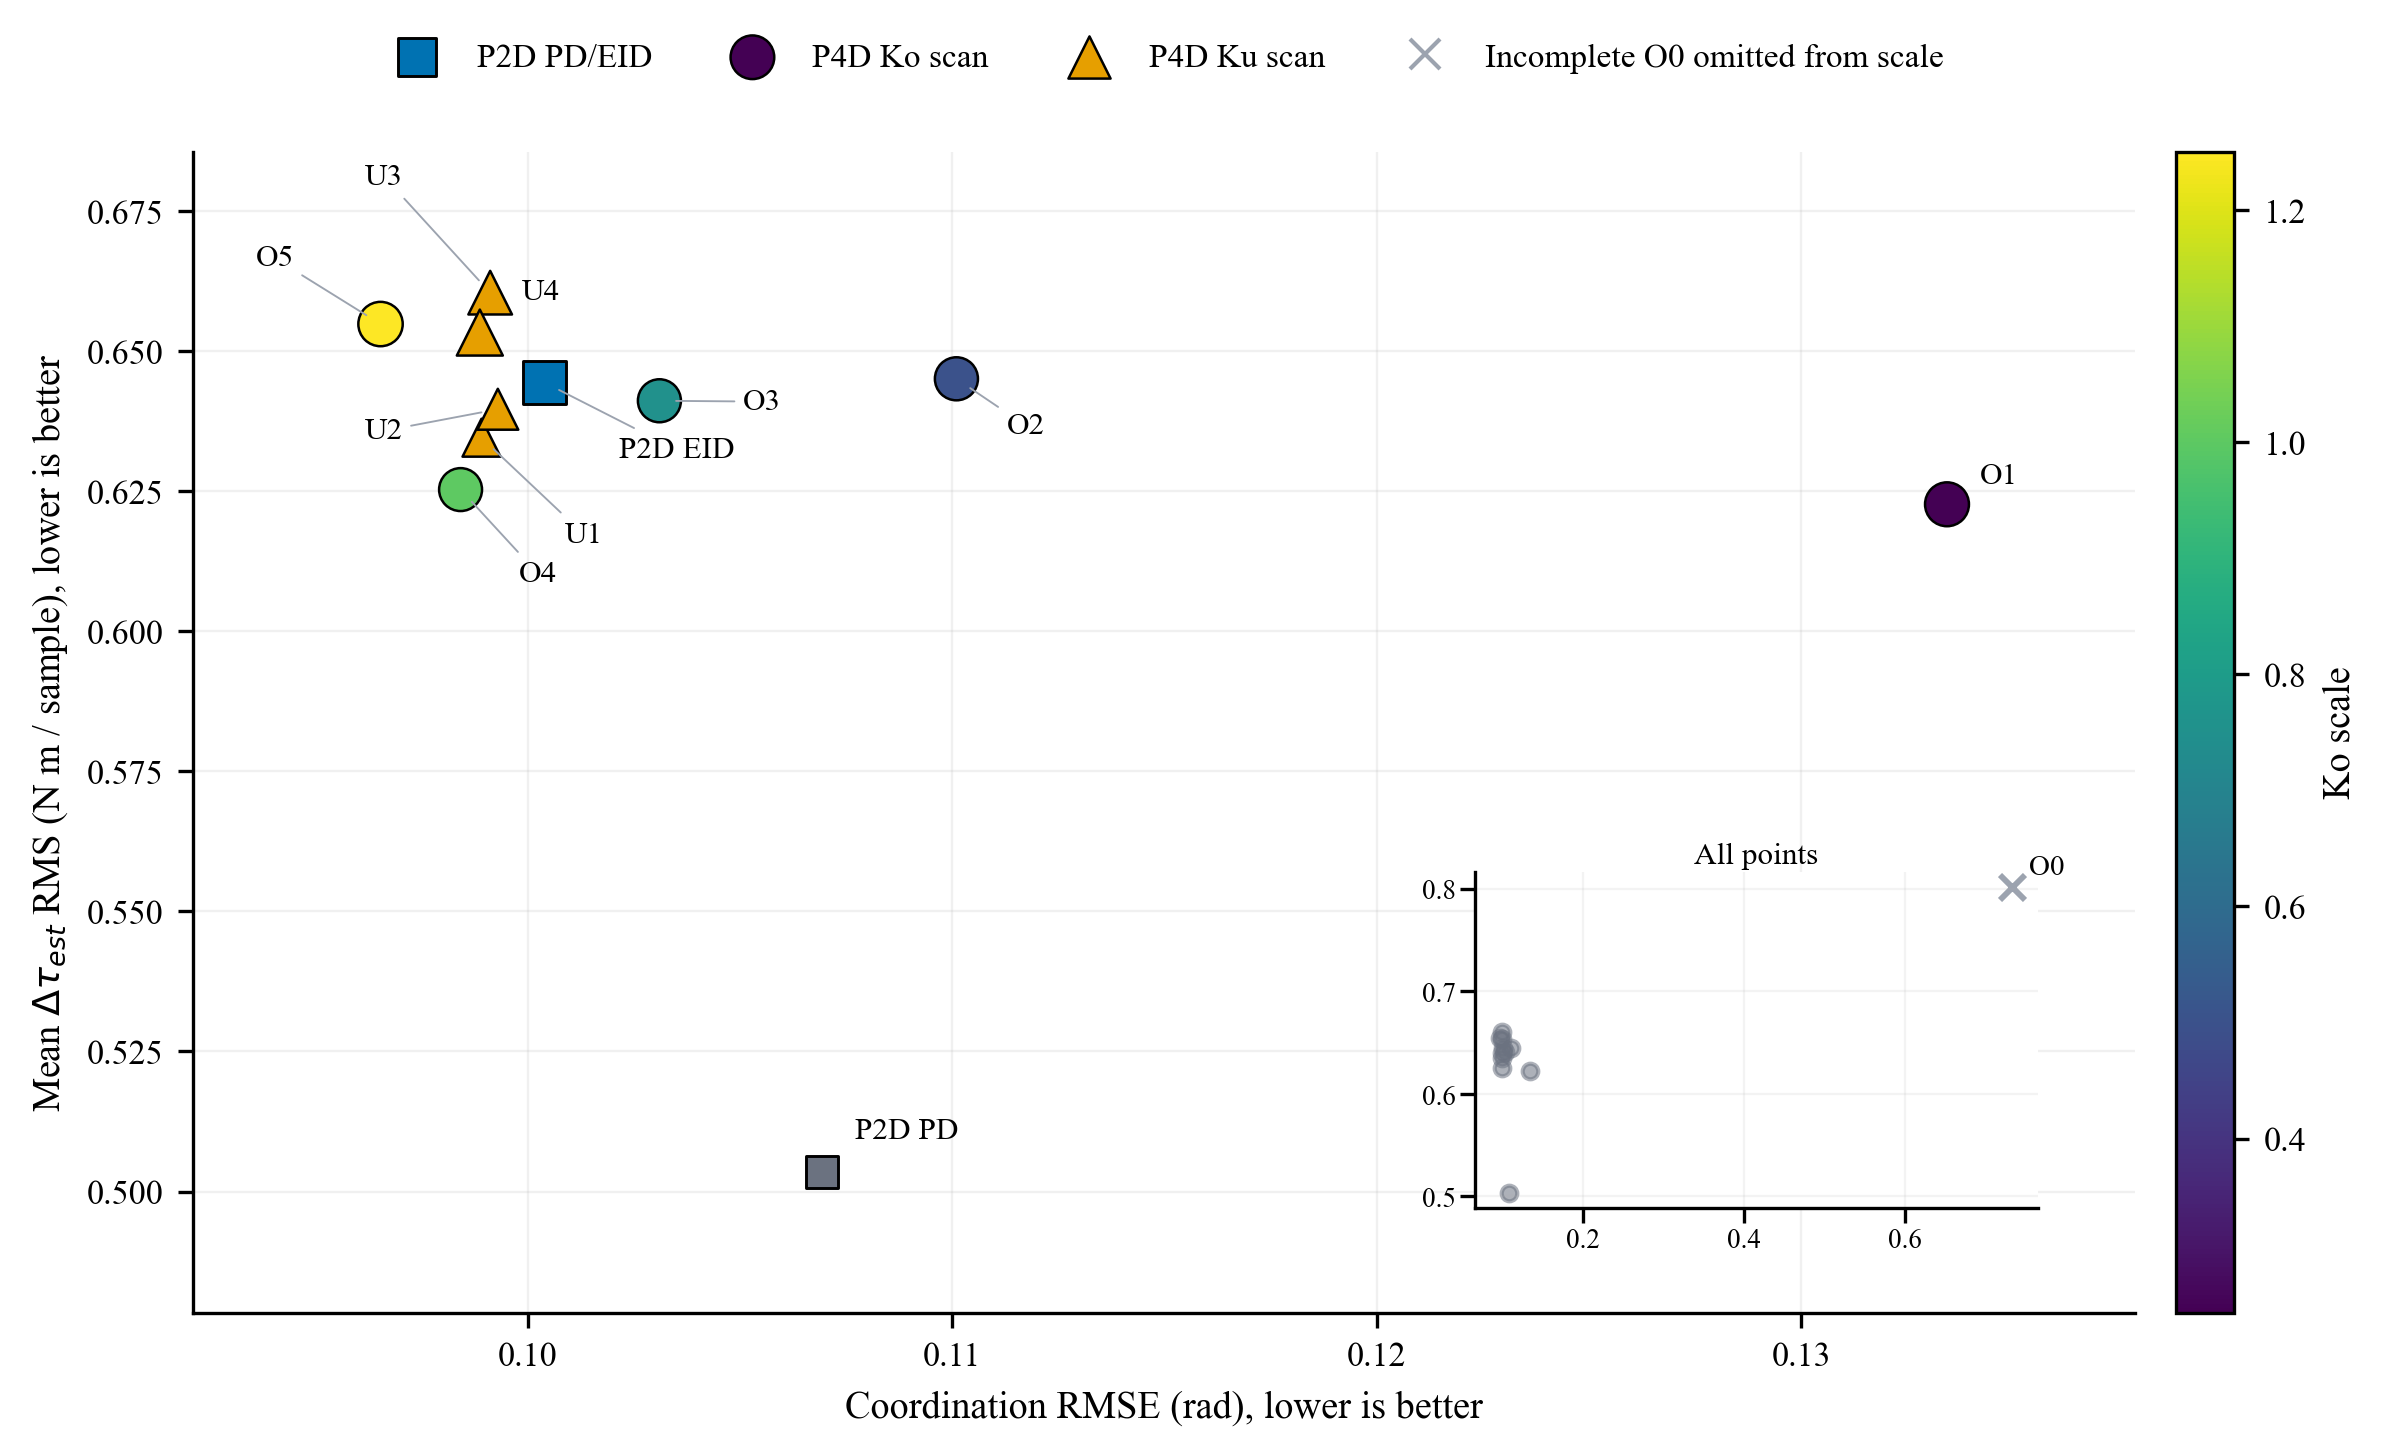
\includegraphics[keepaspectratio,alt={误差收益-力矩代价 Pareto}]{analysis_artifacts/bychen_answer/figures/bychen_tradeoff_pareto.png}}
\caption{误差收益-力矩代价 Pareto}
\end{figure}

\begin{figure}
\centering
\pandocbounded{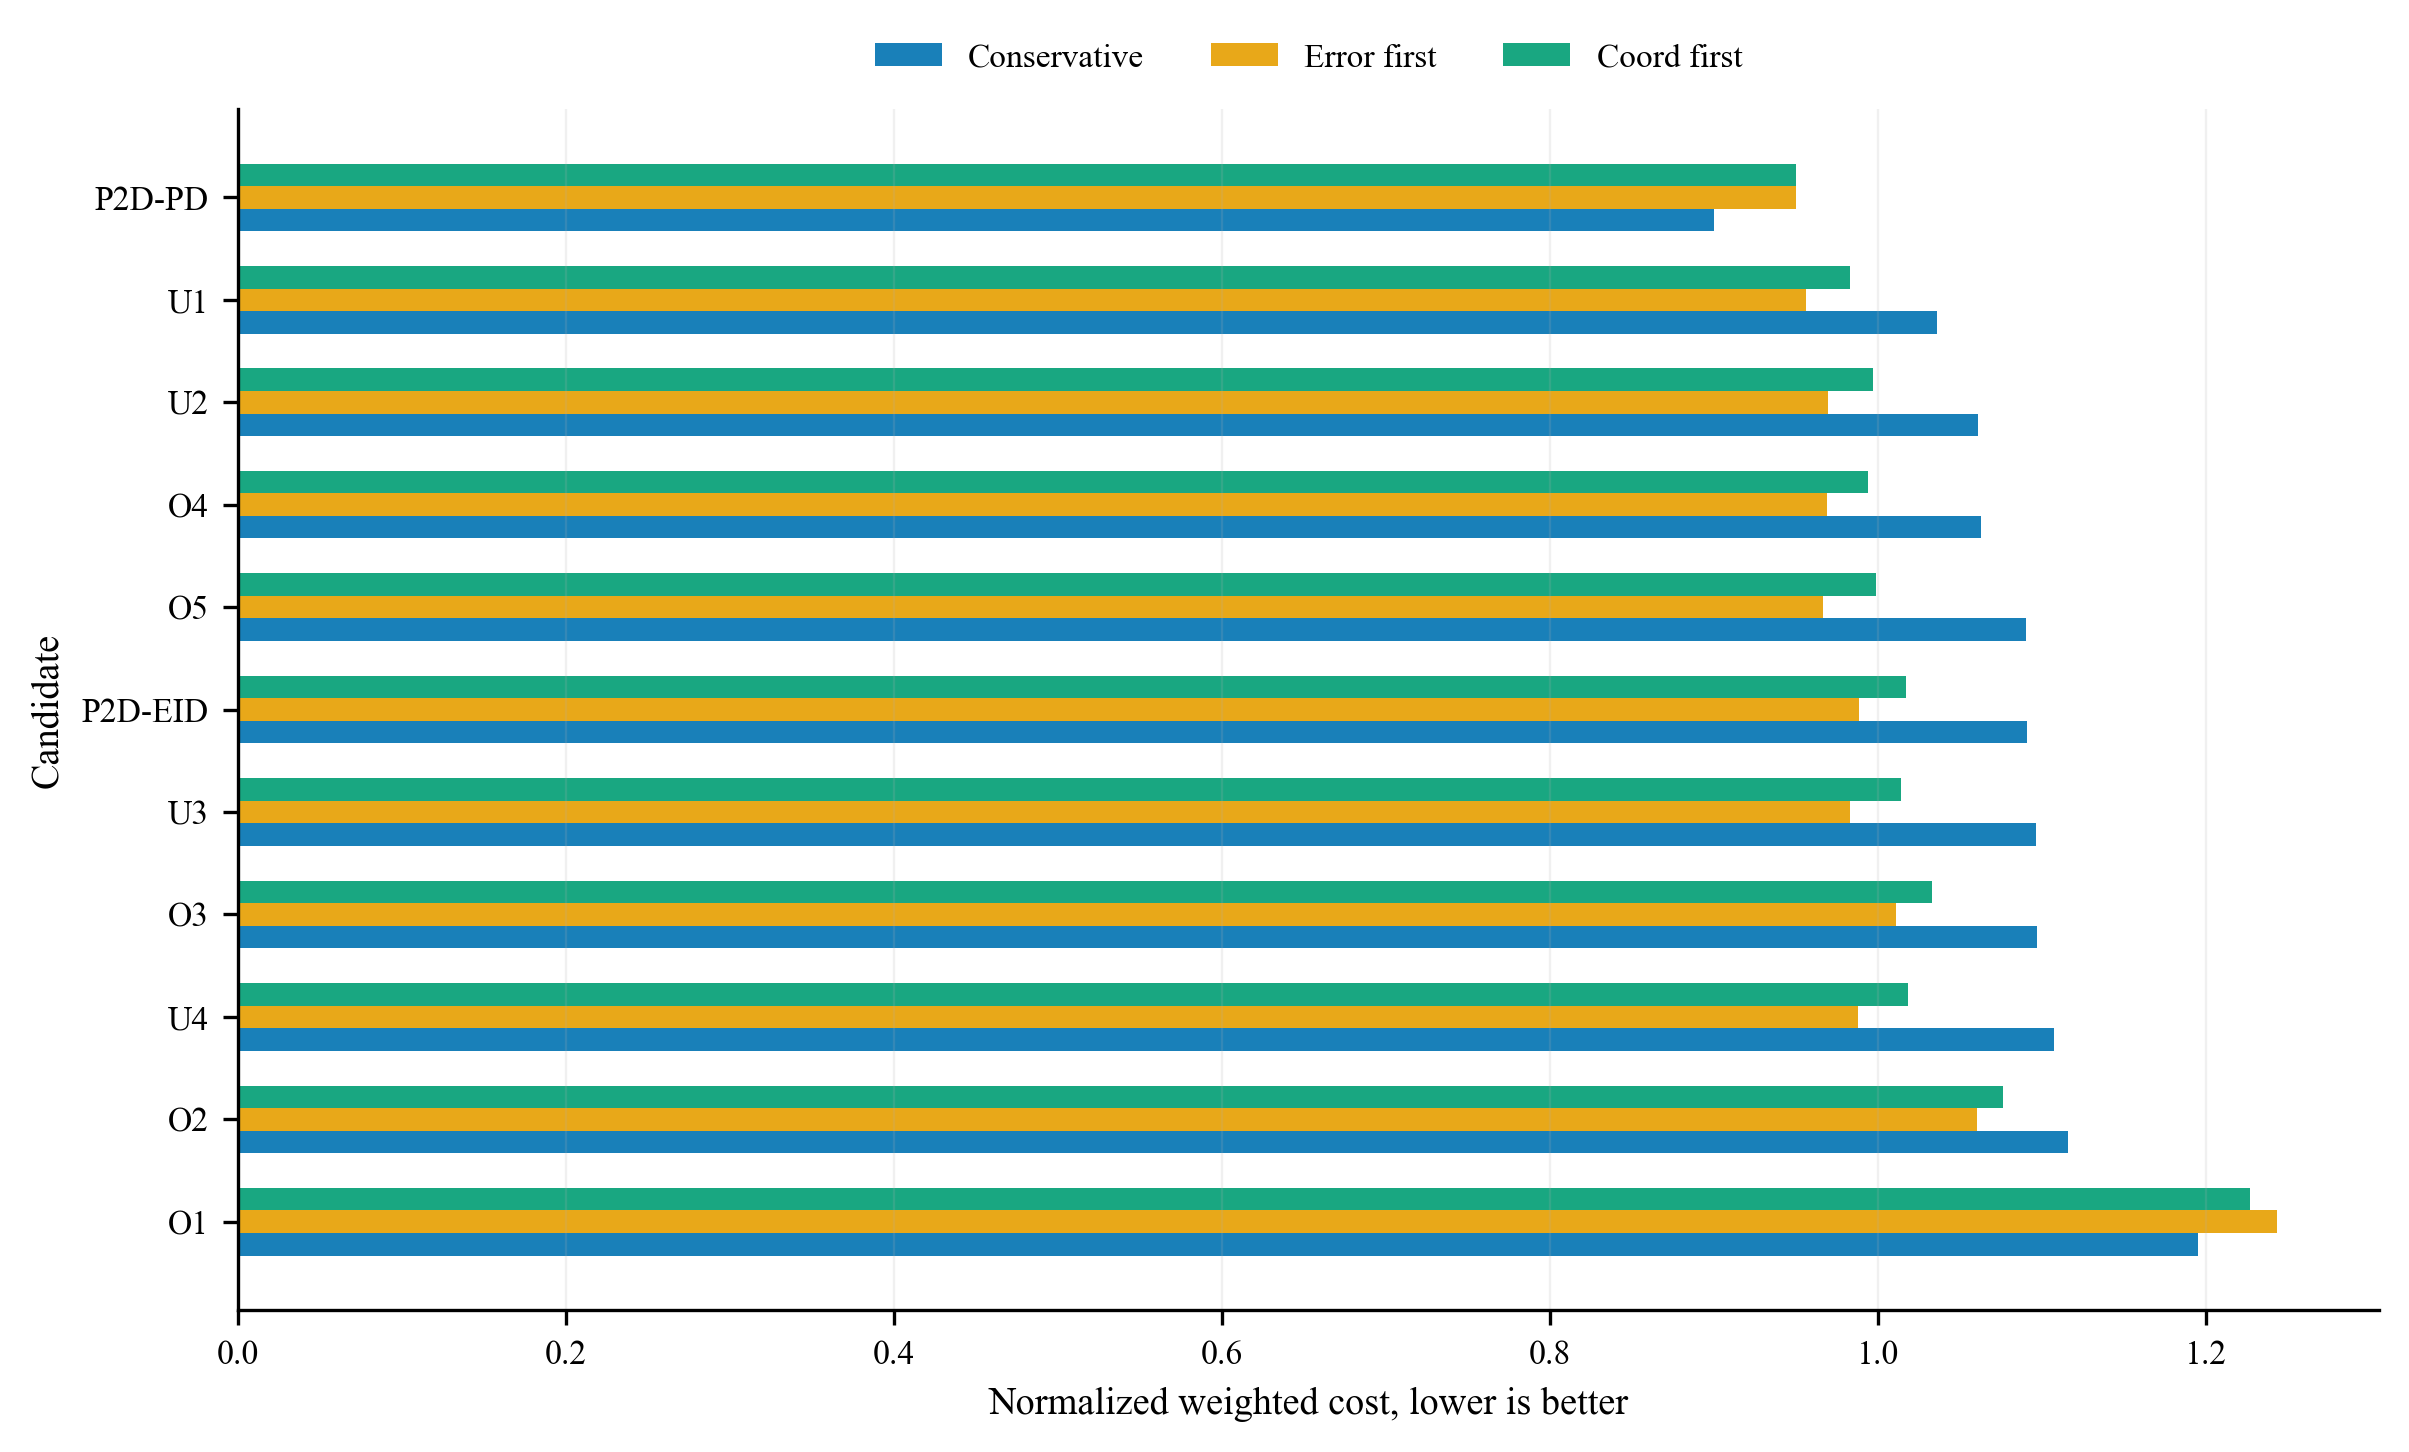
\includegraphics[keepaspectratio,alt={多目标权重敏感性}]{analysis_artifacts/bychen_answer/figures/bychen_multiobjective_sensitivity.png}}
\caption{多目标权重敏感性}
\end{figure}

权重敏感性排名显示，保守权重下 PD 或 U1 排名前列；误差优先权重下 O5 可以前移，但其力矩代价更高。因此参数选择应先给出 Pareto 关系和硬约束，再给出候选排序，而不能宣称唯一最优点。

\section{6. MuJoCo 机制矩阵结果}\label{mujoco-ux673aux5236ux77e9ux9635ux7ed3ux679c}

\subsection{6.1 候选层}\label{ux5019ux9009ux5c42}

MuJoCo 机制矩阵使用真实 C++ \texttt{h1\_controller\_stepper}，协议为 \texttt{8\ s}、\texttt{dt=0.002\ s}、右髋/右膝输入端半余弦等效扰动 \texttt{{[}+6,-4{]}\ N\ m}，时间窗 \texttt{4.0/4.2/5.2/5.4\ s}。

\begin{longtable}[]{@{}
  >{\raggedright\arraybackslash}p{(\linewidth - 14\tabcolsep) * \real{0.1000}}
  >{\raggedright\arraybackslash}p{(\linewidth - 14\tabcolsep) * \real{0.1000}}
  >{\raggedleft\arraybackslash}p{(\linewidth - 14\tabcolsep) * \real{0.1333}}
  >{\raggedleft\arraybackslash}p{(\linewidth - 14\tabcolsep) * \real{0.1333}}
  >{\raggedleft\arraybackslash}p{(\linewidth - 14\tabcolsep) * \real{0.1333}}
  >{\raggedleft\arraybackslash}p{(\linewidth - 14\tabcolsep) * \real{0.1333}}
  >{\raggedleft\arraybackslash}p{(\linewidth - 14\tabcolsep) * \real{0.1333}}
  >{\raggedleft\arraybackslash}p{(\linewidth - 14\tabcolsep) * \real{0.1333}}@{}}
\toprule\noalign{}
\begin{minipage}[b]{\linewidth}\raggedright
候选
\end{minipage} & \begin{minipage}[b]{\linewidth}\raggedright
含义
\end{minipage} & \begin{minipage}[b]{\linewidth}\raggedleft
髋 \texttt{s\_o}
\end{minipage} & \begin{minipage}[b]{\linewidth}\raggedleft
膝 \texttt{s\_o}
\end{minipage} & \begin{minipage}[b]{\linewidth}\raggedleft
协调 RMSE
\end{minipage} & \begin{minipage}[b]{\linewidth}\raggedleft
膝 \texttt{Delta\ tau\_total} RMS
\end{minipage} & \begin{minipage}[b]{\linewidth}\raggedleft
膝 \texttt{eta\_u} RMS
\end{minipage} & \begin{minipage}[b]{\linewidth}\raggedleft
\texttt{combined\_flags}
\end{minipage} \\
\midrule\noalign{}
\endhead
\bottomrule\noalign{}
\endlastfoot
A / \texttt{A\_O4U1} & \texttt{O4+U1} 保守基线：标称观测器倍率 + 弱输入补偿 & 1.00 & 1.00 & 0.067562 & 0.137295 & 0.015854 & 4 \\
B / \texttt{B\_HipUp} & 只提高髋观测器倍率 & 1.25 & 1.00 & 0.067200 & 0.137283 & 0.015856 & 4 \\
D / \texttt{D\_HipUpKneeDown} & 髋增强、膝减弱 & 1.25 & 0.75 & 0.069233 & 0.135377 & 0.016195 & 4 \\
E / \texttt{O5U1} & \texttt{O5+U1}：髋膝共同高观测器倍率 + 弱输入补偿 & 1.25 & 1.25 & 0.065995 & 0.138420 & 0.015655 & 4 \\
\texttt{KneeVelDown} & 只降低膝速度观测器通道，膝位置通道保持 1.00 & 1.00 & 位置 1.00，速度 0.75 & 0.069429 & 0.135514 & 0.016194 & 4 \\
\end{longtable}

\begin{figure}
\centering
\pandocbounded{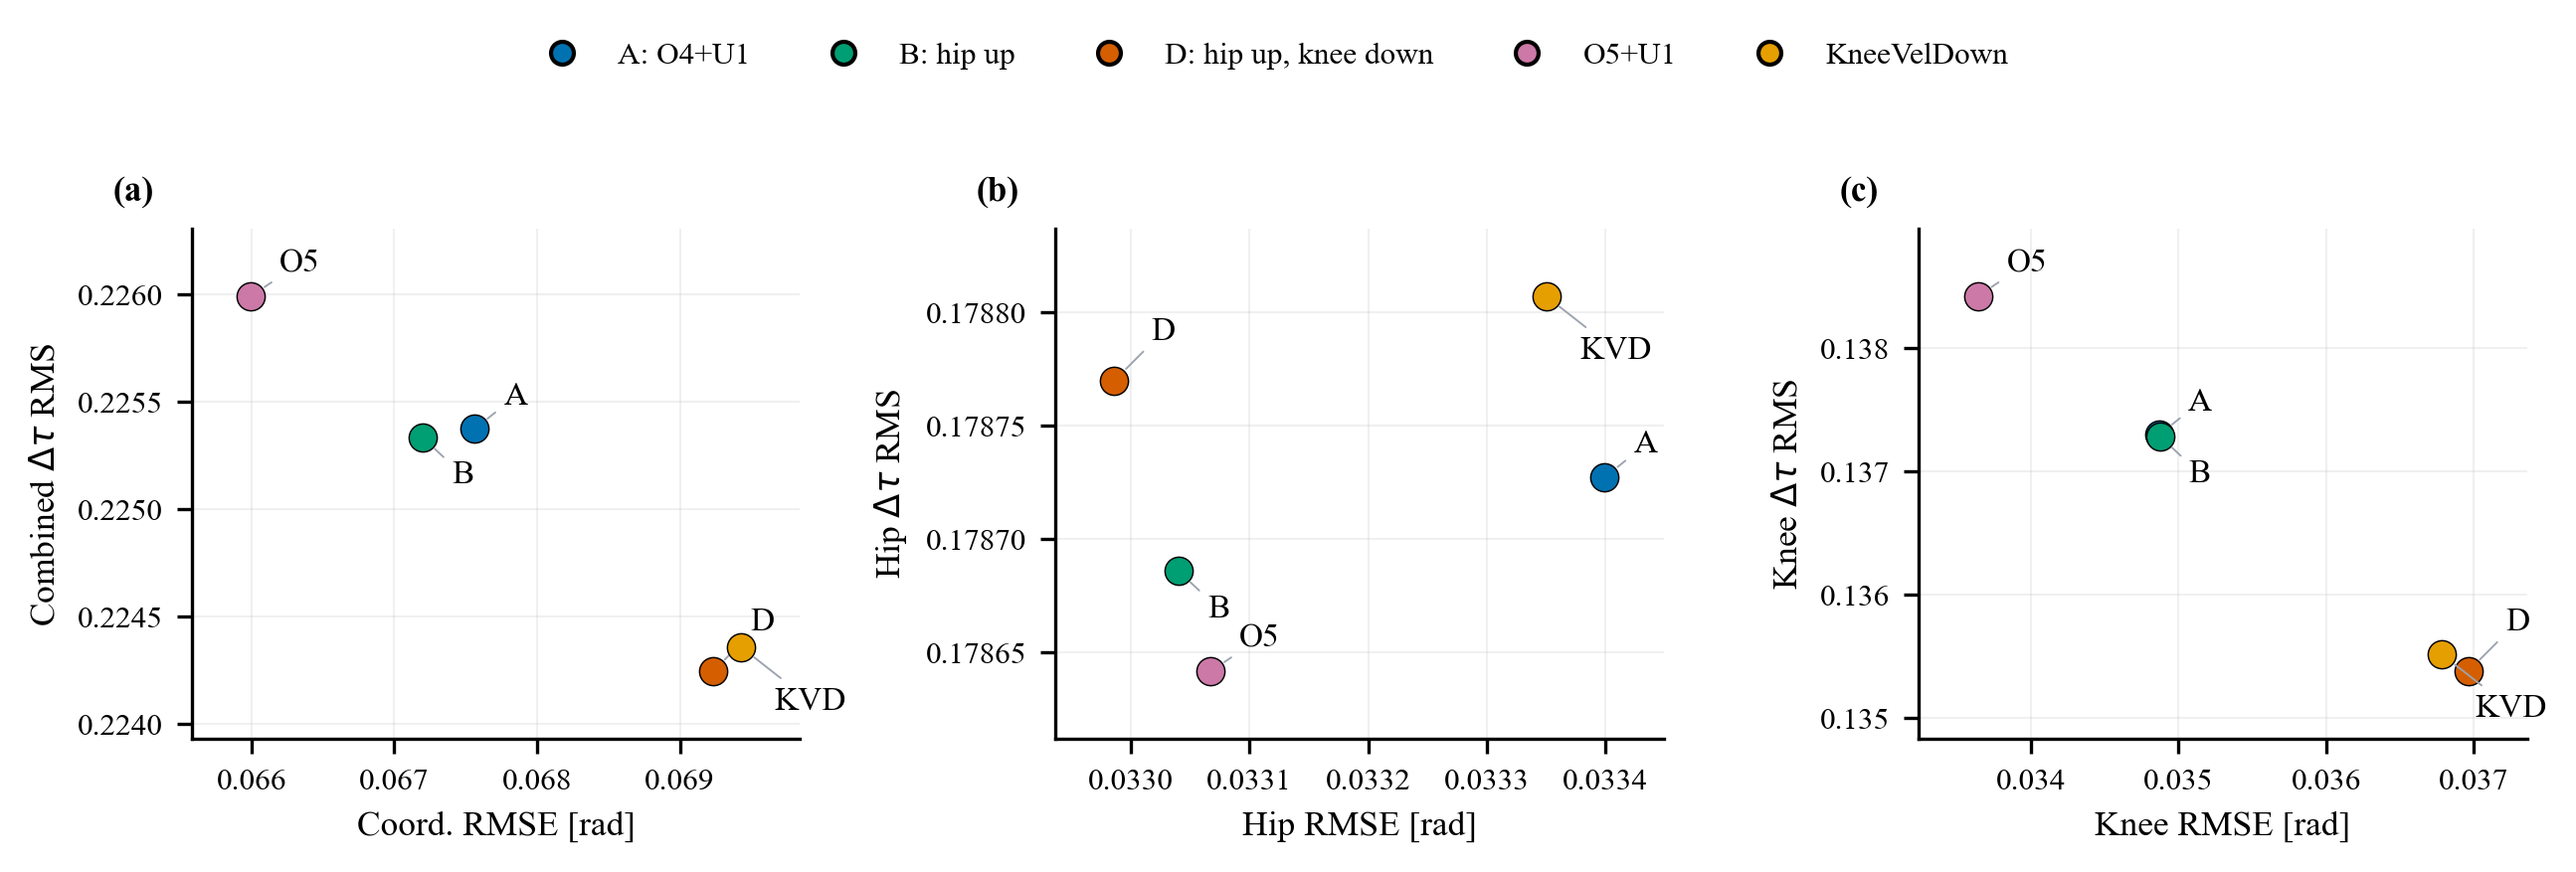
\includegraphics[keepaspectratio,alt={MuJoCo 机制矩阵候选 Pareto}]{analysis_artifacts/bychen_mujoco_mechanism_completion/figures/mujoco_mechanism_candidate_pareto.png}}
\caption{MuJoCo 机制矩阵候选 Pareto}
\end{figure}

相对 A（\texttt{A\_O4U1}，保守基线）：

\begin{itemize}
\tightlist
\item
  E（\texttt{O5U1} / \texttt{O5+U1}）协调 RMSE 下降约 2.32\%，但膝 \texttt{Delta\ tau\_total} RMS 上升约 0.82\%。
\item
  B（只提高髋观测器倍率）协调 RMSE 下降约 0.54\%，膝力矩变化量几乎不变，是更保守的上机候选。
\item
  D（髋增强、膝减弱）和 \texttt{KneeVelDown} 分别使膝 \texttt{Delta\ tau\_total} RMS 降低约 1.40\% 和 1.30\%，但协调 RMSE 分别上升约 2.47\% 和 2.76\%。
\end{itemize}

\textbf{结论。} MuJoCo 支持把 B（只提高髋观测器倍率）和 E（\texttt{O5+U1}）作为优先实机候选，把 D（髋增强、膝减弱）或 \texttt{KneeVelDown} 作为膝力矩活动机制验证点。它不支持把 D 预写成最优。

\subsection{6.2 候选层频谱}\label{ux5019ux9009ux5c42ux9891ux8c31}

\begin{longtable}[]{@{}
  >{\raggedright\arraybackslash}p{(\linewidth - 8\tabcolsep) * \real{0.1667}}
  >{\raggedright\arraybackslash}p{(\linewidth - 8\tabcolsep) * \real{0.1667}}
  >{\raggedleft\arraybackslash}p{(\linewidth - 8\tabcolsep) * \real{0.2222}}
  >{\raggedleft\arraybackslash}p{(\linewidth - 8\tabcolsep) * \real{0.2222}}
  >{\raggedleft\arraybackslash}p{(\linewidth - 8\tabcolsep) * \real{0.2222}}@{}}
\toprule\noalign{}
\begin{minipage}[b]{\linewidth}\raggedright
候选
\end{minipage} & \begin{minipage}[b]{\linewidth}\raggedright
信号
\end{minipage} & \begin{minipage}[b]{\linewidth}\raggedleft
峰值频率 Hz
\end{minipage} & \begin{minipage}[b]{\linewidth}\raggedleft
0.5--3 Hz 带功率
\end{minipage} & \begin{minipage}[b]{\linewidth}\raggedleft
15--80 Hz 带功率
\end{minipage} \\
\midrule\noalign{}
\endhead
\bottomrule\noalign{}
\endlastfoot
A（保守基线） & \texttt{coord\_error} & 0.9766 & 1.113e-4 & 6.768e-8 \\
A（保守基线） & \texttt{knee\_delta\_tau\_total} & 20.5078 & 1.590e-4 & 2.2926e-2 \\
B（髋增强） & \texttt{coord\_error} & 0.9766 & 1.116e-4 & 6.751e-8 \\
B（髋增强） & \texttt{knee\_delta\_tau\_total} & 20.5078 & 1.598e-4 & 2.2923e-2 \\
D（髋增、膝减） & \texttt{coord\_error} & 0.9766 & 1.127e-4 & 6.569e-8 \\
D（髋增、膝减） & \texttt{knee\_delta\_tau\_total} & 20.5078 & 1.553e-4 & 2.2245e-2 \\
E（\texttt{O5+U1}） & \texttt{coord\_error} & 0.9766 & 1.112e-4 & 6.824e-8 \\
E（\texttt{O5+U1}） & \texttt{knee\_delta\_tau\_total} & 20.5078 & 1.625e-4 & 2.3359e-2 \\
\end{longtable}

\begin{figure}
\centering
\pandocbounded{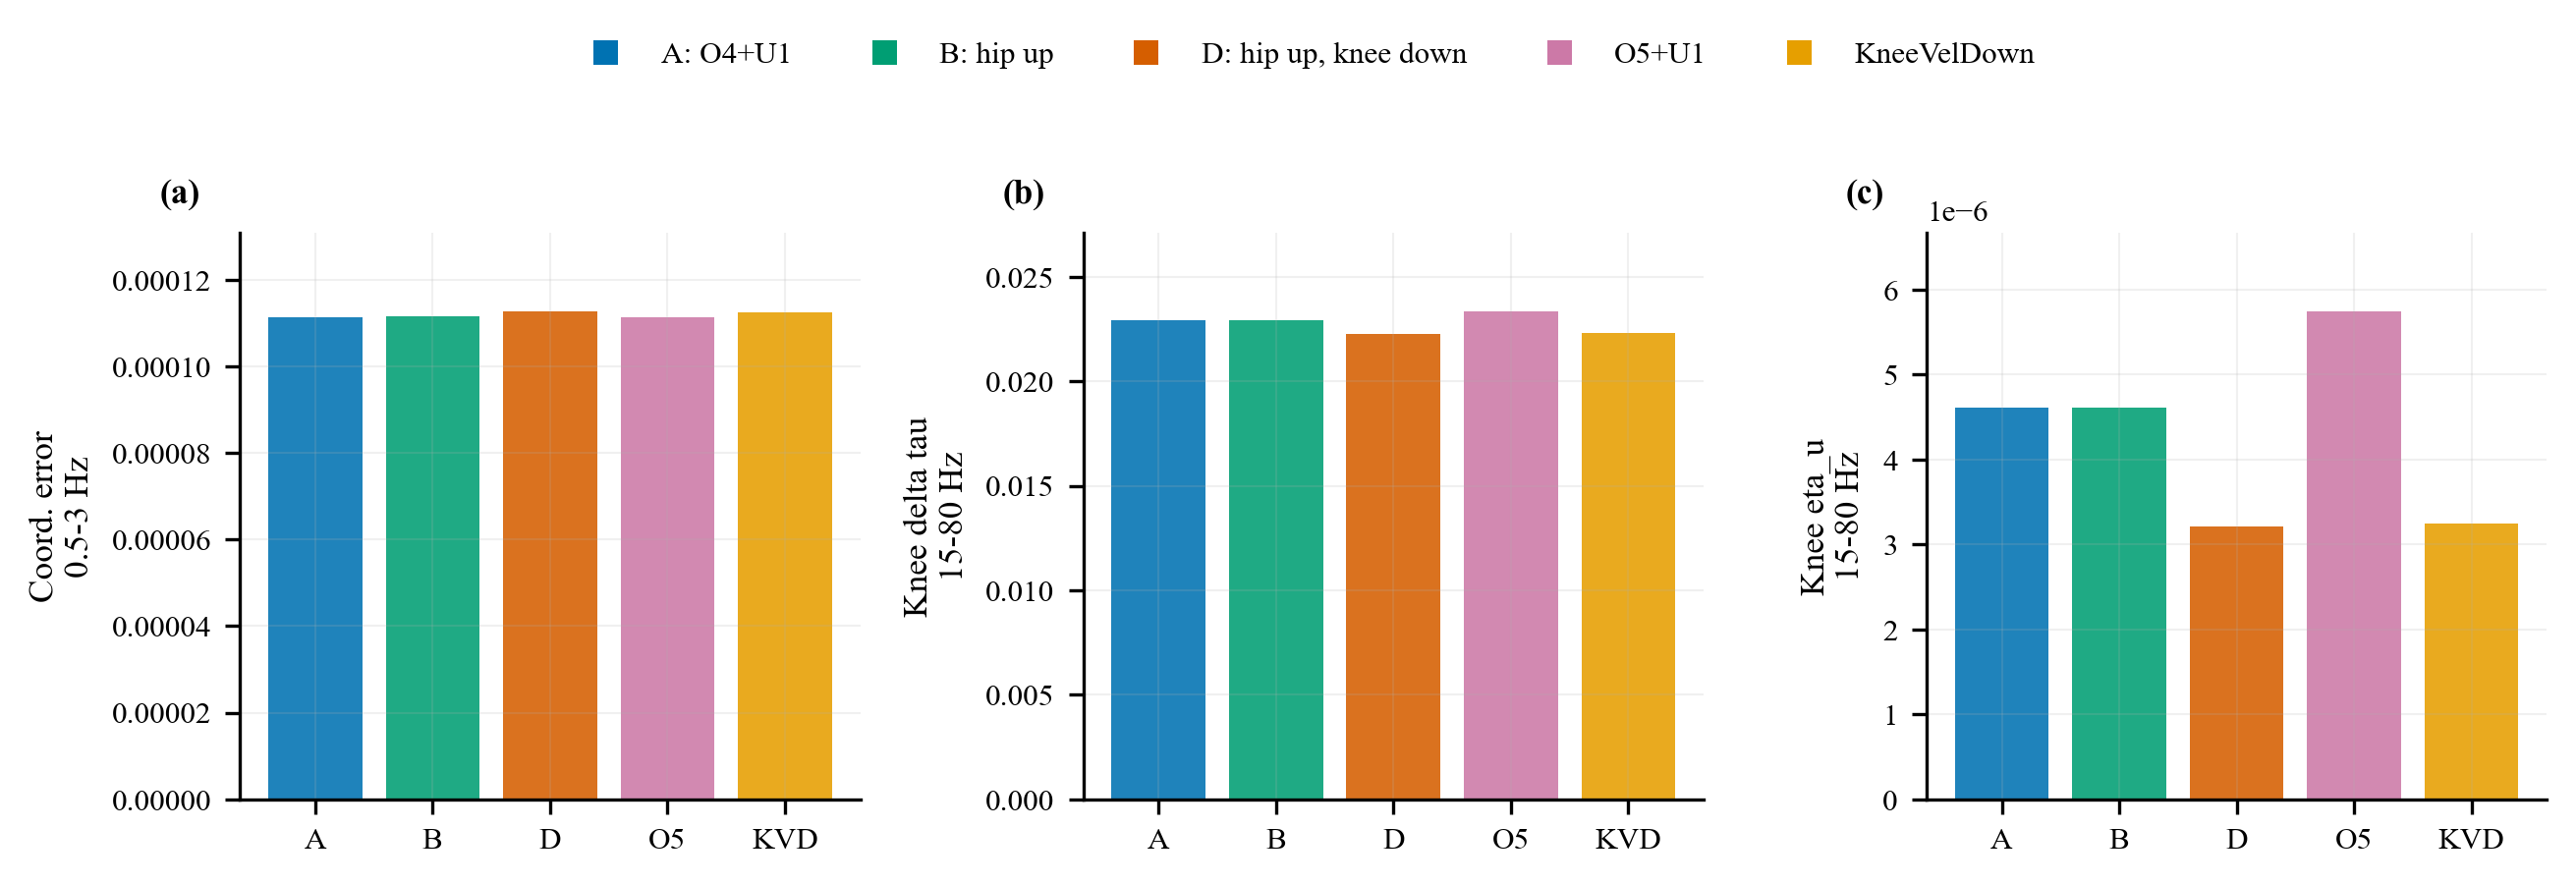
\includegraphics[keepaspectratio,alt={MuJoCo 机制矩阵频谱摘要}]{analysis_artifacts/bychen_mujoco_mechanism_completion/figures/mujoco_mechanism_spectrum_summary.png}}
\caption{MuJoCo 机制矩阵频谱摘要}
\end{figure}

\textbf{结论。} 提高观测器倍率更偏向误差收益，降低膝速度/整体膝观测器倍率更偏向膝力矩活动约束；二者在当前数据里不能同时最优。

\subsection{6.3 结构消融}\label{ux7ed3ux6784ux6d88ux878d}

\begin{longtable}[]{@{}
  >{\raggedright\arraybackslash}p{(\linewidth - 10\tabcolsep) * \real{0.1364}}
  >{\raggedright\arraybackslash}p{(\linewidth - 10\tabcolsep) * \real{0.1364}}
  >{\raggedleft\arraybackslash}p{(\linewidth - 10\tabcolsep) * \real{0.1818}}
  >{\raggedleft\arraybackslash}p{(\linewidth - 10\tabcolsep) * \real{0.1818}}
  >{\raggedleft\arraybackslash}p{(\linewidth - 10\tabcolsep) * \real{0.1818}}
  >{\raggedleft\arraybackslash}p{(\linewidth - 10\tabcolsep) * \real{0.1818}}@{}}
\toprule\noalign{}
\begin{minipage}[b]{\linewidth}\raggedright
候选
\end{minipage} & \begin{minipage}[b]{\linewidth}\raggedright
\texttt{eid\_mode}
\end{minipage} & \begin{minipage}[b]{\linewidth}\raggedleft
协调 RMSE
\end{minipage} & \begin{minipage}[b]{\linewidth}\raggedleft
膝 \texttt{Delta\ tau\_total} RMS
\end{minipage} & \begin{minipage}[b]{\linewidth}\raggedleft
膝 \texttt{eta\_u} RMS
\end{minipage} & \begin{minipage}[b]{\linewidth}\raggedleft
恢复段协调 RMSE
\end{minipage} \\
\midrule\noalign{}
\endhead
\bottomrule\noalign{}
\endlastfoot
O4+U1 & \texttt{pd\_inverse\_only} & 0.059987 & 0.132226 & 0.000000 & 0.017111 \\
O4+U1 & \texttt{center\_feedback\_only} & 0.067726 & 0.137277 & 0.000000 & 0.018157 \\
O4+U1 & \texttt{input\_compensation\_only} & 0.059821 & 0.132180 & 0.015753 & 0.017092 \\
O4+U1 & \texttt{full\_eid} & 0.067562 & 0.137295 & 0.015854 & 0.018133 \\
O5+U1 & \texttt{pd\_inverse\_only} & 0.059987 & 0.132226 & 0.000000 & 0.017111 \\
O5+U1 & \texttt{center\_feedback\_only} & 0.066155 & 0.138418 & 0.000000 & 0.017941 \\
O5+U1 & \texttt{input\_compensation\_only} & 0.059822 & 0.132128 & 0.015572 & 0.017092 \\
O5+U1 & \texttt{full\_eid} & 0.065995 & 0.138420 & 0.015655 & 0.017918 \\
\end{longtable}

\begin{figure}
\centering
\pandocbounded{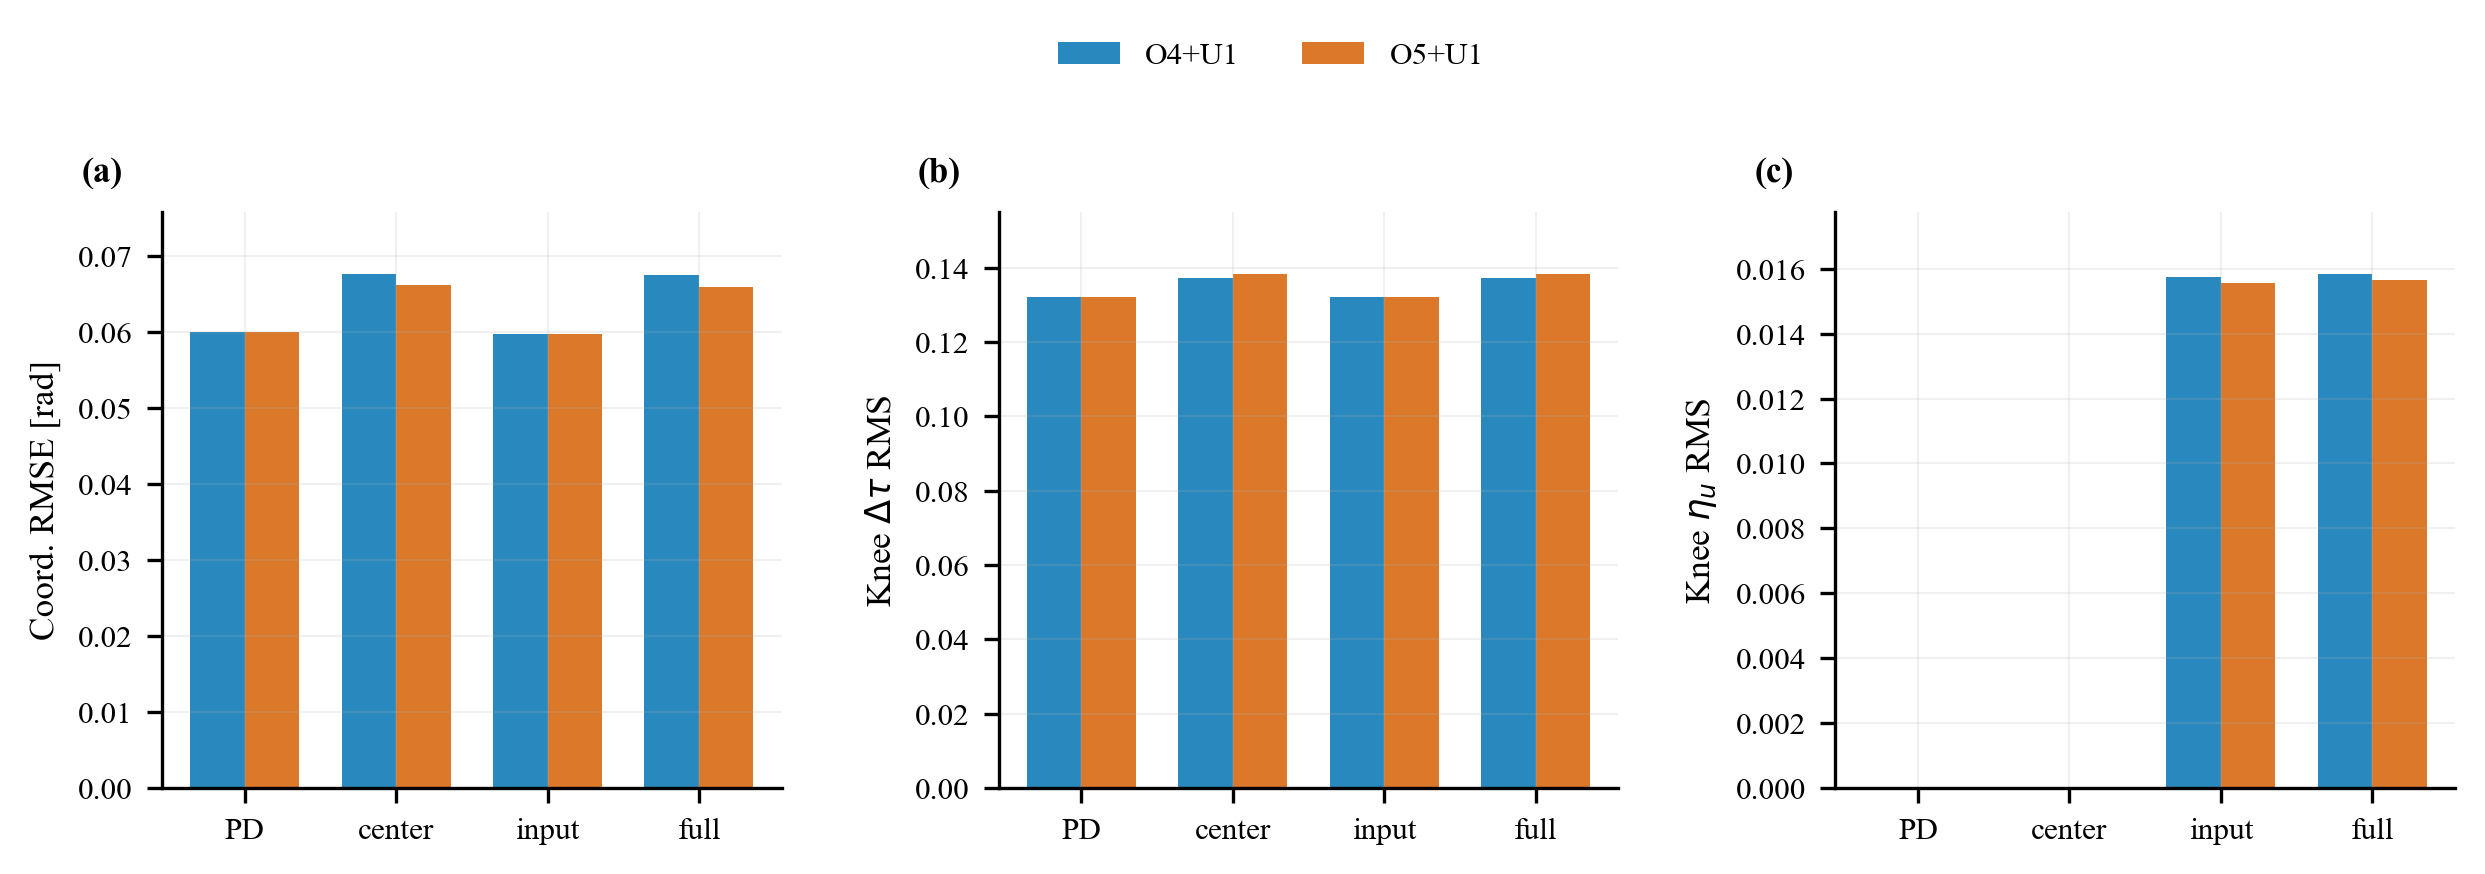
\includegraphics[keepaspectratio,alt={MuJoCo 真实 stepper 结构消融}]{analysis_artifacts/bychen_mujoco_mechanism_completion/figures/mujoco_mechanism_structure_ablation.png}}
\caption{MuJoCo 真实 stepper 结构消融}
\end{figure}

\textbf{结论。} \texttt{input\_compensation\_only} 与 \texttt{pd\_inverse\_only} 的协调 RMSE 非常接近，说明 \texttt{K\_u\ eta} 直接输入补偿不是主要 RMSE 杠杆；\texttt{center\_feedback\_only} 与 \texttt{full\_eid} 接近，说明完整 EID 的主要动态变化来自 \texttt{xbar=\textbackslash{}hat\{x\}+\textbackslash{}eta} 反馈中心。

\subsection{\texorpdfstring{6.4 残差 \texttt{lambda} 扫描}{6.4 残差 lambda 扫描}}\label{ux6b8bux5dee-lambda-ux626bux63cf}

当前完整 EID 使用：

\[
r_k=x_k-\hat{x}_{k|k-1}-\eta_{k|k-1}.
\]

新 stepper 实现混合残差：

\[
r_k(\lambda)=x_k-\hat{x}_{k|k-1}-\lambda\eta_{k|k-1},
\qquad
\lambda\in\{0,0.5,1\}.
\]

\begin{longtable}[]{@{}
  >{\raggedright\arraybackslash}p{(\linewidth - 10\tabcolsep) * \real{0.1304}}
  >{\raggedleft\arraybackslash}p{(\linewidth - 10\tabcolsep) * \real{0.1739}}
  >{\raggedleft\arraybackslash}p{(\linewidth - 10\tabcolsep) * \real{0.1739}}
  >{\raggedleft\arraybackslash}p{(\linewidth - 10\tabcolsep) * \real{0.1739}}
  >{\raggedleft\arraybackslash}p{(\linewidth - 10\tabcolsep) * \real{0.1739}}
  >{\raggedleft\arraybackslash}p{(\linewidth - 10\tabcolsep) * \real{0.1739}}@{}}
\toprule\noalign{}
\begin{minipage}[b]{\linewidth}\raggedright
候选
\end{minipage} & \begin{minipage}[b]{\linewidth}\raggedleft
\texttt{lambda}
\end{minipage} & \begin{minipage}[b]{\linewidth}\raggedleft
协调 RMSE
\end{minipage} & \begin{minipage}[b]{\linewidth}\raggedleft
膝 \texttt{Delta\ tau\_total} RMS
\end{minipage} & \begin{minipage}[b]{\linewidth}\raggedleft
膝 \texttt{eta\_u} RMS
\end{minipage} & \begin{minipage}[b]{\linewidth}\raggedleft
\texttt{combined\_flags}
\end{minipage} \\
\midrule\noalign{}
\endhead
\bottomrule\noalign{}
\endlastfoot
O4+U1 & 0.0 & 0.065733 & 0.138952 & 0.015668 & 4 \\
O4+U1 & 0.5 & 0.066631 & 0.138136 & 0.015760 & 4 \\
O4+U1 & 1.0 & 0.067562 & 0.137295 & 0.015854 & 4 \\
O5+U1 & 0.0 & 0.064238 & 0.139901 & 0.015483 & 4 \\
O5+U1 & 0.5 & 0.065104 & 0.139192 & 0.015565 & 4 \\
O5+U1 & 1.0 & 0.065995 & 0.138420 & 0.015655 & 4 \\
\end{longtable}

\begin{figure}
\centering
\pandocbounded{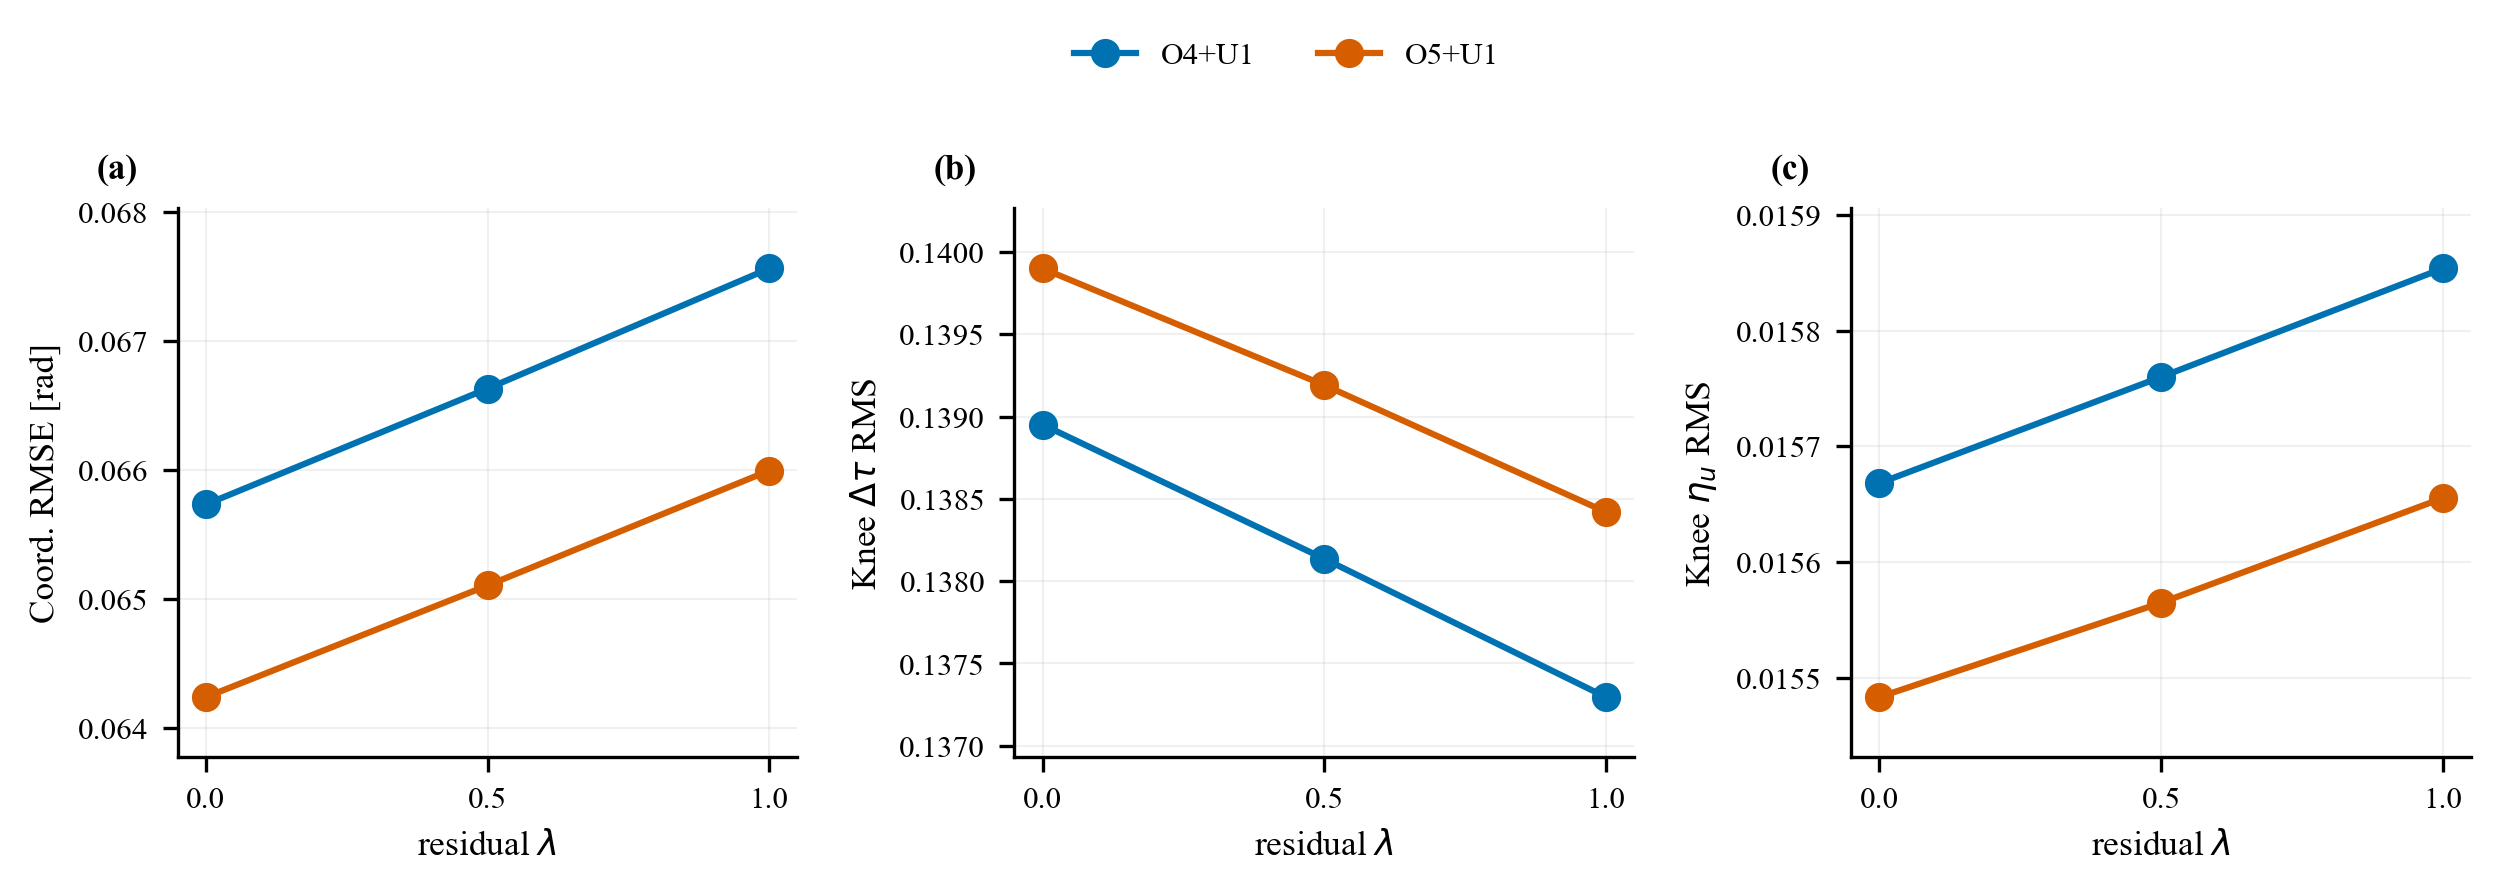
\includegraphics[keepaspectratio,alt={MuJoCo 残差 lambda 扫描}]{analysis_artifacts/bychen_mujoco_mechanism_completion/figures/mujoco_mechanism_residual_lambda.png}}
\caption{MuJoCo 残差 lambda 扫描}
\end{figure}

\textbf{结论。} \texttt{lambda} 越小，协调 RMSE 越低，但膝 \texttt{Delta\ tau\_total} RMS 越高。残差定义不是``越激进越好''，而是误差与力矩活动之间的结构性权衡。\texttt{lambda=0} 或 \texttt{0.5} 不应直接上机，应先在 MuJoCo 中叠加测量噪声和更严格执行器限幅。

\section{7. MuJoCo 日志频谱、coherence 与经验 FRF}\label{mujoco-ux65e5ux5fd7ux9891ux8c31coherence-ux4e0eux7ecfux9a8c-frf}

A--D 四组 MuJoCo 日志的 PSD 和 coherence 已完成。这里的 A--D 沿用第 0.4 节的候选矩阵命名：A 是 \texttt{O4+U1} 保守基线，B 是髋增强，C 是膝减弱，D 是髋增、膝减。

\begin{longtable}[]{@{}
  >{\raggedright\arraybackslash}p{(\linewidth - 6\tabcolsep) * \real{0.2000}}
  >{\raggedleft\arraybackslash}p{(\linewidth - 6\tabcolsep) * \real{0.2667}}
  >{\raggedleft\arraybackslash}p{(\linewidth - 6\tabcolsep) * \real{0.2667}}
  >{\raggedleft\arraybackslash}p{(\linewidth - 6\tabcolsep) * \real{0.2667}}@{}}
\toprule\noalign{}
\begin{minipage}[b]{\linewidth}\raggedright
组别
\end{minipage} & \begin{minipage}[b]{\linewidth}\raggedleft
\texttt{e\_coord} 峰值 Hz
\end{minipage} & \begin{minipage}[b]{\linewidth}\raggedleft
膝 \texttt{Delta\ tau\_total} 峰值 Hz
\end{minipage} & \begin{minipage}[b]{\linewidth}\raggedleft
膝 \texttt{eta\_u} 15--80 Hz 带功率
\end{minipage} \\
\midrule\noalign{}
\endhead
\bottomrule\noalign{}
\endlastfoot
A（保守基线） & 0.9766 & 20.5078 & 4.6076e-6 \\
B（髋增强） & 0.9766 & 20.5078 & 4.6079e-6 \\
C（膝减弱） & 0.9766 & 20.5078 & 3.2146e-6 \\
D（髋增、膝减） & 0.9766 & 20.5078 & 3.2156e-6 \\
\end{longtable}

\begin{figure}
\centering
\pandocbounded{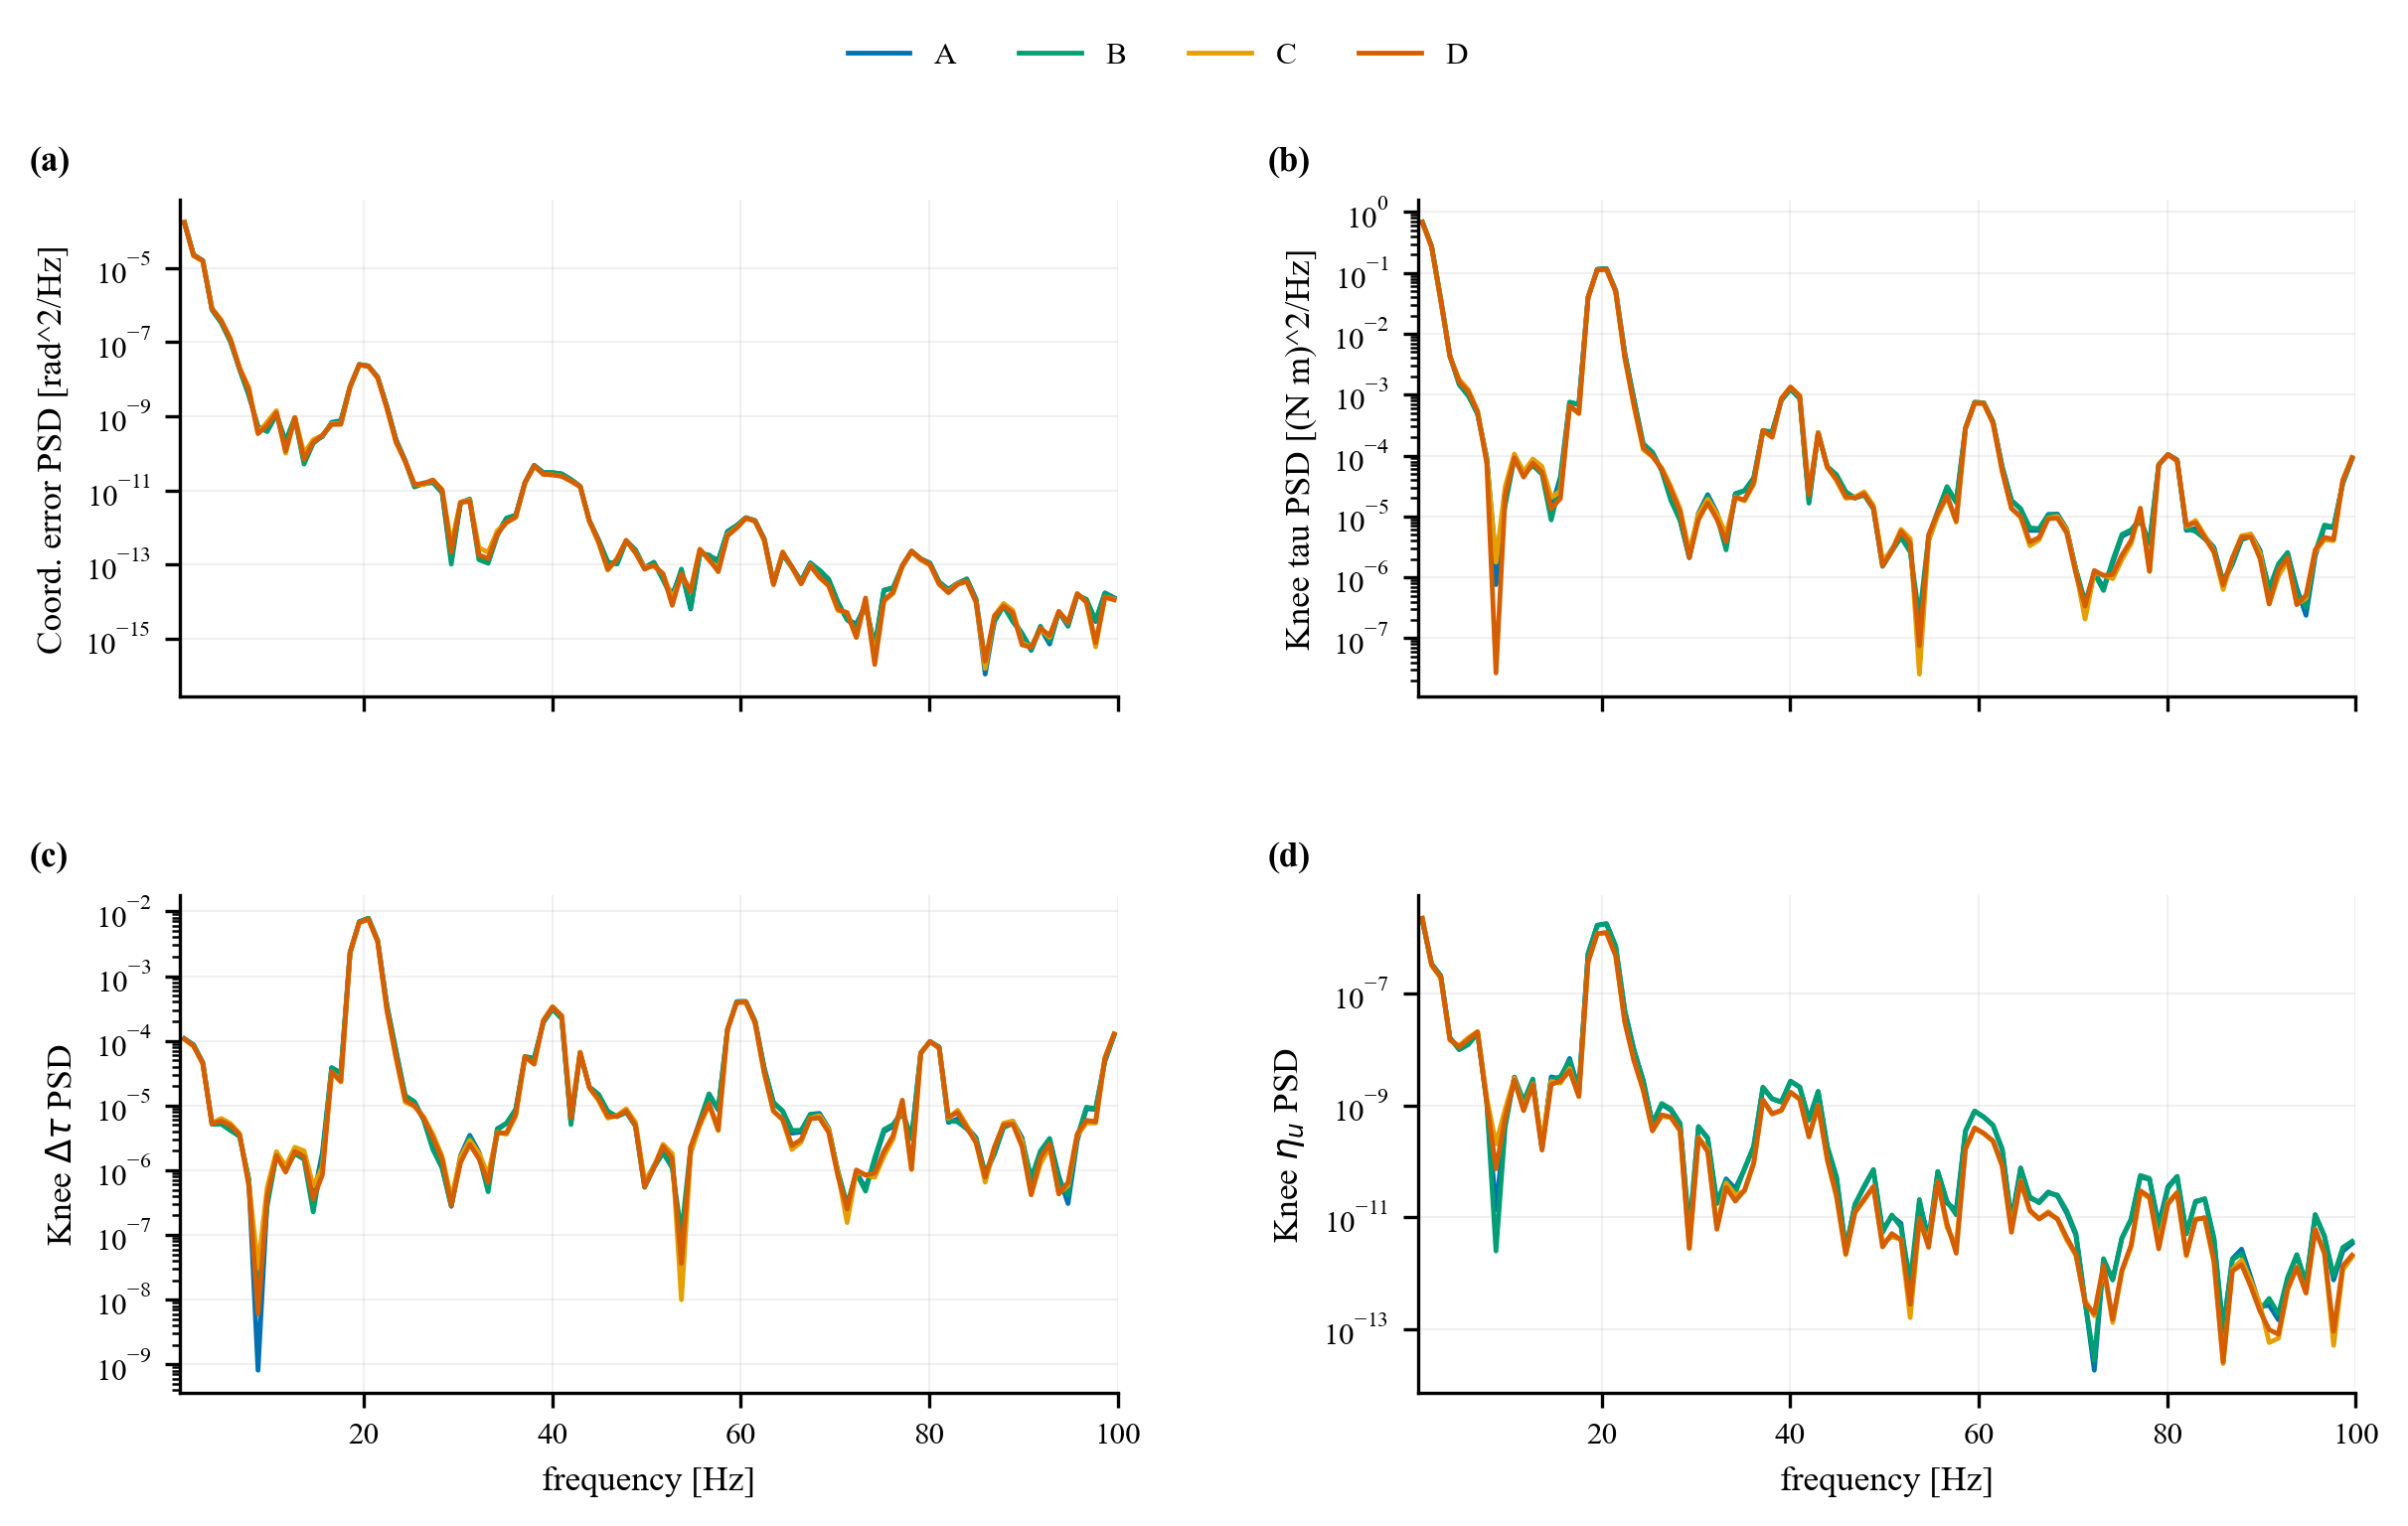
\includegraphics[keepaspectratio,alt={MuJoCo 日志 PSD}]{analysis_artifacts/bychen_mujoco_sweep/mujoco_deep_analysis/figures/bychen_mujoco_log_psd.png}}
\caption{MuJoCo 日志 PSD}
\end{figure}

扰动到协调误差的 coherence：

\begin{longtable}[]{@{}lrrr@{}}
\toprule\noalign{}
组别 & coherence 峰值频率 Hz & 峰值 coherence & 峰值相位 rad \\
\midrule\noalign{}
\endhead
\bottomrule\noalign{}
\endlastfoot
A（保守基线） & 5.859 & 0.9777 & 1.9278 \\
B（髋增强） & 5.859 & 0.9778 & 1.9332 \\
C（膝减弱） & 5.859 & 0.9783 & 1.9285 \\
D（髋增、膝减） & 5.859 & 0.9788 & 1.9350 \\
\end{longtable}

\begin{figure}
\centering
\pandocbounded{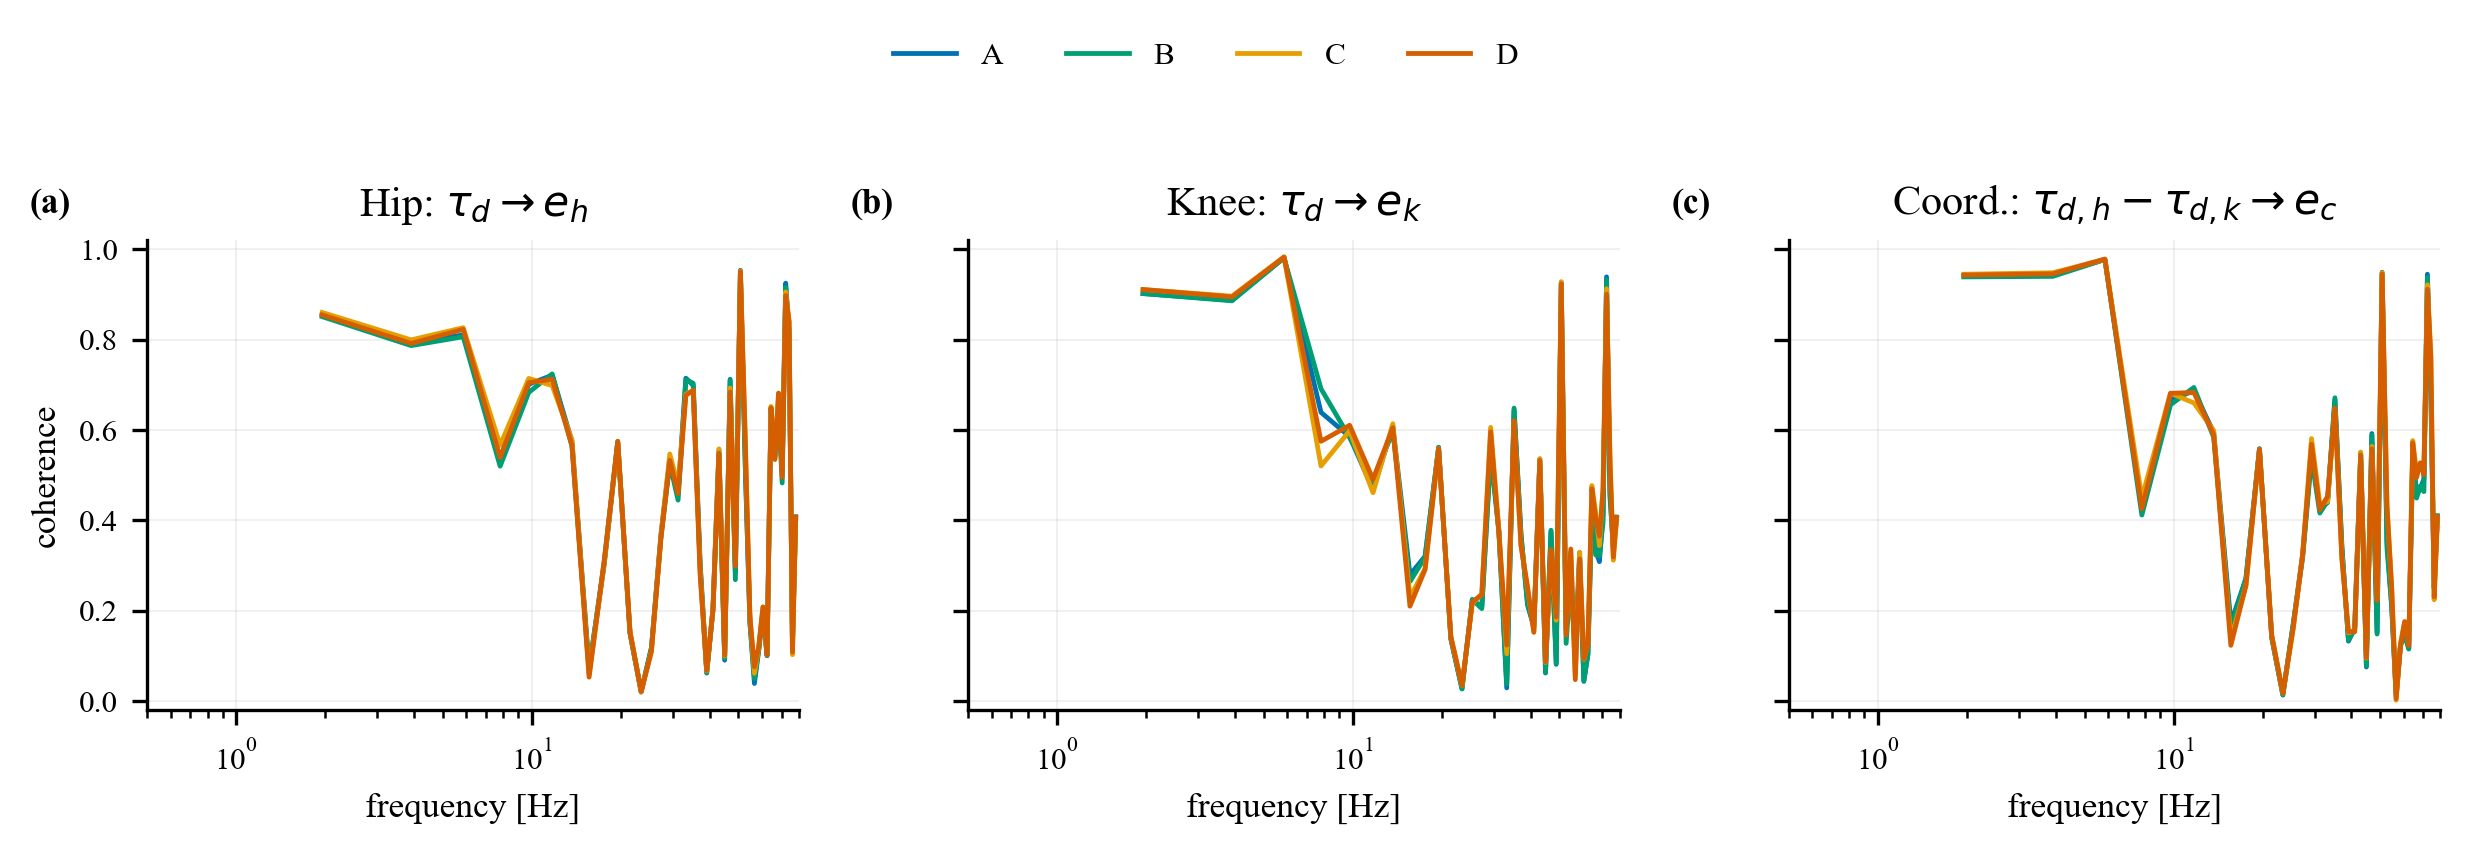
\includegraphics[keepaspectratio,alt={MuJoCo 扰动 coherence}]{analysis_artifacts/bychen_mujoco_sweep/mujoco_deep_analysis/figures/bychen_mujoco_disturbance_coherence.png}}
\caption{MuJoCo 扰动 coherence}
\end{figure}

经验 FRF 的幅值峰在约 18.55 Hz，但该点 coherence 约 0.038--0.040，低于 95\% 阈值 0.348。因此，不能只按经验 FRF 幅值峰解释控制规律，必须联看 coherence。

\begin{figure}
\centering
\pandocbounded{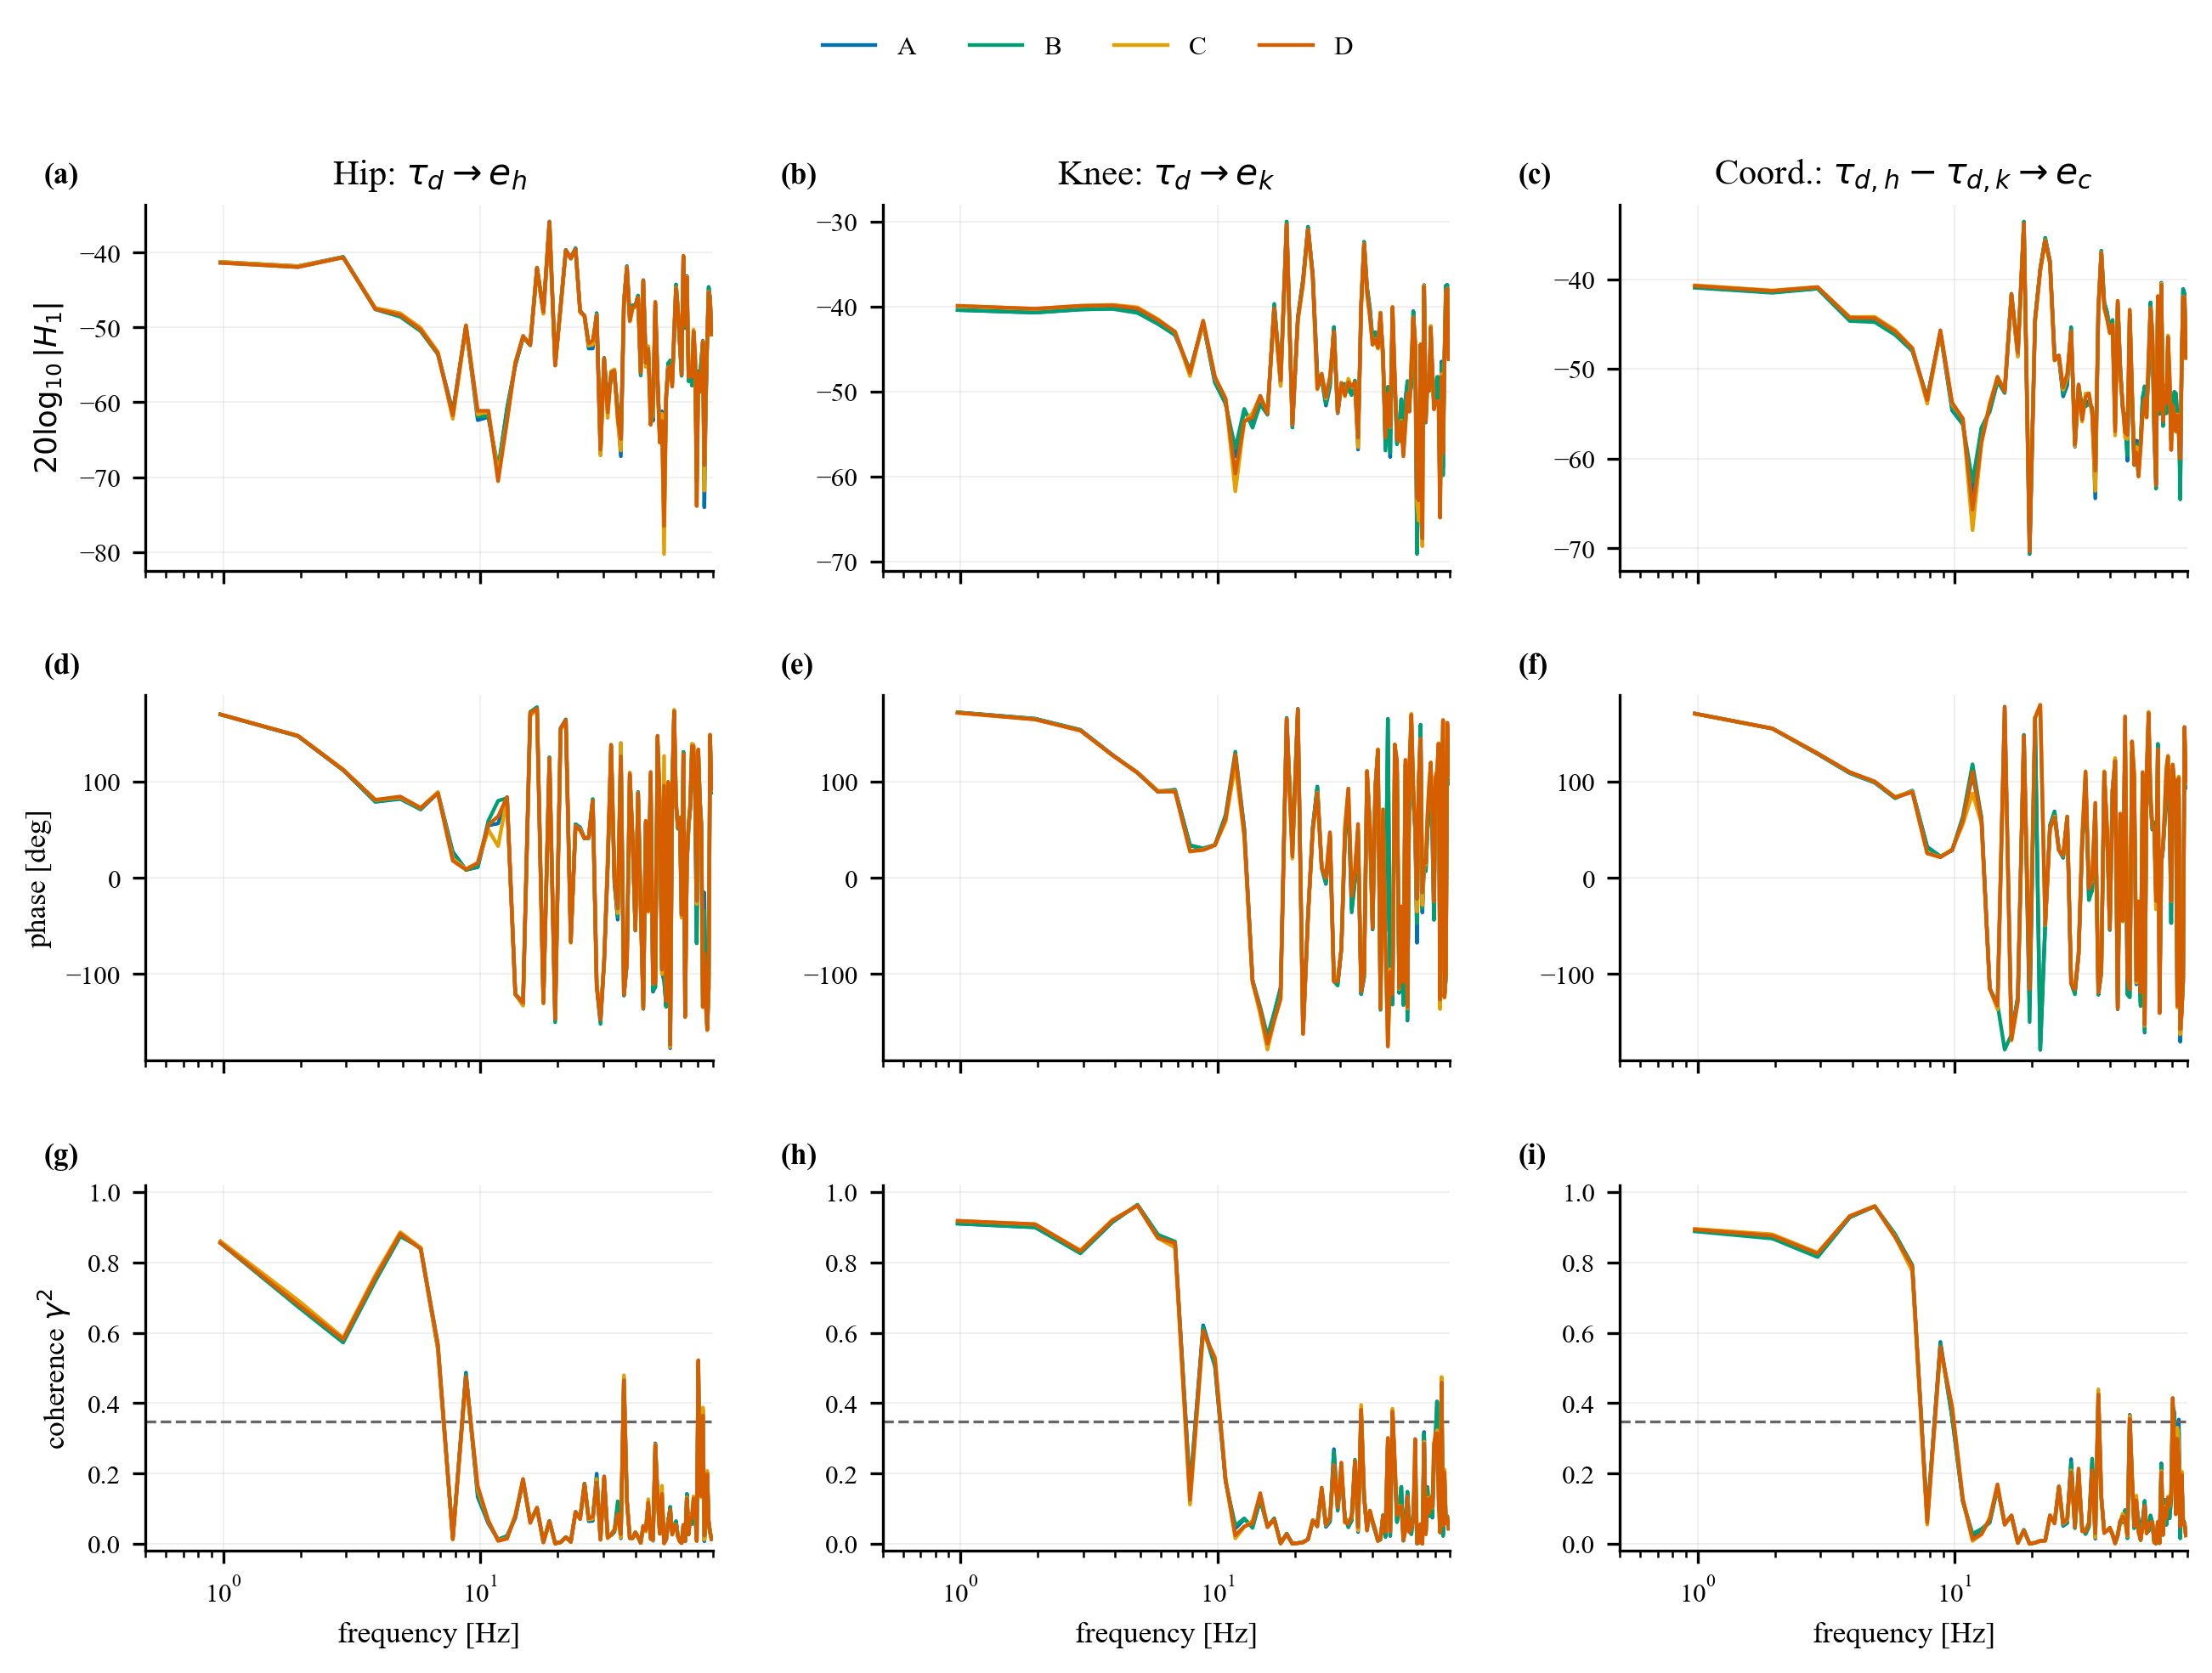
\includegraphics[keepaspectratio,alt={MuJoCo 闭环日志经验 FRF/Bode}]{analysis_artifacts/bychen_mujoco_sweep/mujoco_deep_analysis/figures/bychen_mujoco_empirical_frf_bode.png}}
\caption{MuJoCo 闭环日志经验 FRF/Bode}
\end{figure}

\section{8. 局部辨识增广闭环与频响}\label{ux5c40ux90e8ux8fa8ux8bc6ux589eux5e7fux95edux73afux4e0eux9891ux54cd}

\subsection{8.1 MuJoCo 局部离散 plant}\label{mujoco-ux5c40ux90e8ux79bbux6563-plant}

从 A--D 候选的 MuJoCo 日志中辨识局部离散单关节模型，其中 A/B/C/D 的含义与第 7 节相同：

\[
\delta x_{k+1}=A_{\rm mj}\delta x_k+B_{\rm mj}\delta u_k,
\qquad
x=[q,\dot q]^\top .
\]

\begin{longtable}[]{@{}
  >{\raggedright\arraybackslash}p{(\linewidth - 16\tabcolsep) * \real{0.0857}}
  >{\raggedleft\arraybackslash}p{(\linewidth - 16\tabcolsep) * \real{0.1143}}
  >{\raggedleft\arraybackslash}p{(\linewidth - 16\tabcolsep) * \real{0.1143}}
  >{\raggedleft\arraybackslash}p{(\linewidth - 16\tabcolsep) * \real{0.1143}}
  >{\raggedleft\arraybackslash}p{(\linewidth - 16\tabcolsep) * \real{0.1143}}
  >{\raggedleft\arraybackslash}p{(\linewidth - 16\tabcolsep) * \real{0.1143}}
  >{\raggedleft\arraybackslash}p{(\linewidth - 16\tabcolsep) * \real{0.1143}}
  >{\raggedleft\arraybackslash}p{(\linewidth - 16\tabcolsep) * \real{0.1143}}
  >{\raggedleft\arraybackslash}p{(\linewidth - 16\tabcolsep) * \real{0.1143}}@{}}
\toprule\noalign{}
\begin{minipage}[b]{\linewidth}\raggedright
关节
\end{minipage} & \begin{minipage}[b]{\linewidth}\raggedleft
\texttt{A11}
\end{minipage} & \begin{minipage}[b]{\linewidth}\raggedleft
\texttt{A12}
\end{minipage} & \begin{minipage}[b]{\linewidth}\raggedleft
\texttt{A21}
\end{minipage} & \begin{minipage}[b]{\linewidth}\raggedleft
\texttt{A22}
\end{minipage} & \begin{minipage}[b]{\linewidth}\raggedleft
\texttt{B1}
\end{minipage} & \begin{minipage}[b]{\linewidth}\raggedleft
\texttt{B2}
\end{minipage} & \begin{minipage}[b]{\linewidth}\raggedleft
\texttt{R2\_q}
\end{minipage} & \begin{minipage}[b]{\linewidth}\raggedleft
\texttt{R2\_dq}
\end{minipage} \\
\midrule\noalign{}
\endhead
\bottomrule\noalign{}
\endlastfoot
Hip & 1.00000 & 0.001986 & 0.002258 & 0.993186 & 1.2126e-5 & 0.006063 & 1.00000 & 0.999993 \\
Knee & 0.999953 & 0.001971 & -0.023326 & 0.985465 & 2.9990e-5 & 0.014995 & 1.00000 & 0.999990 \\
\end{longtable}

\subsection{8.2 局部增广闭环极点}\label{ux5c40ux90e8ux589eux5e7fux95edux73afux6781ux70b9}

\begin{figure}
\centering
\pandocbounded{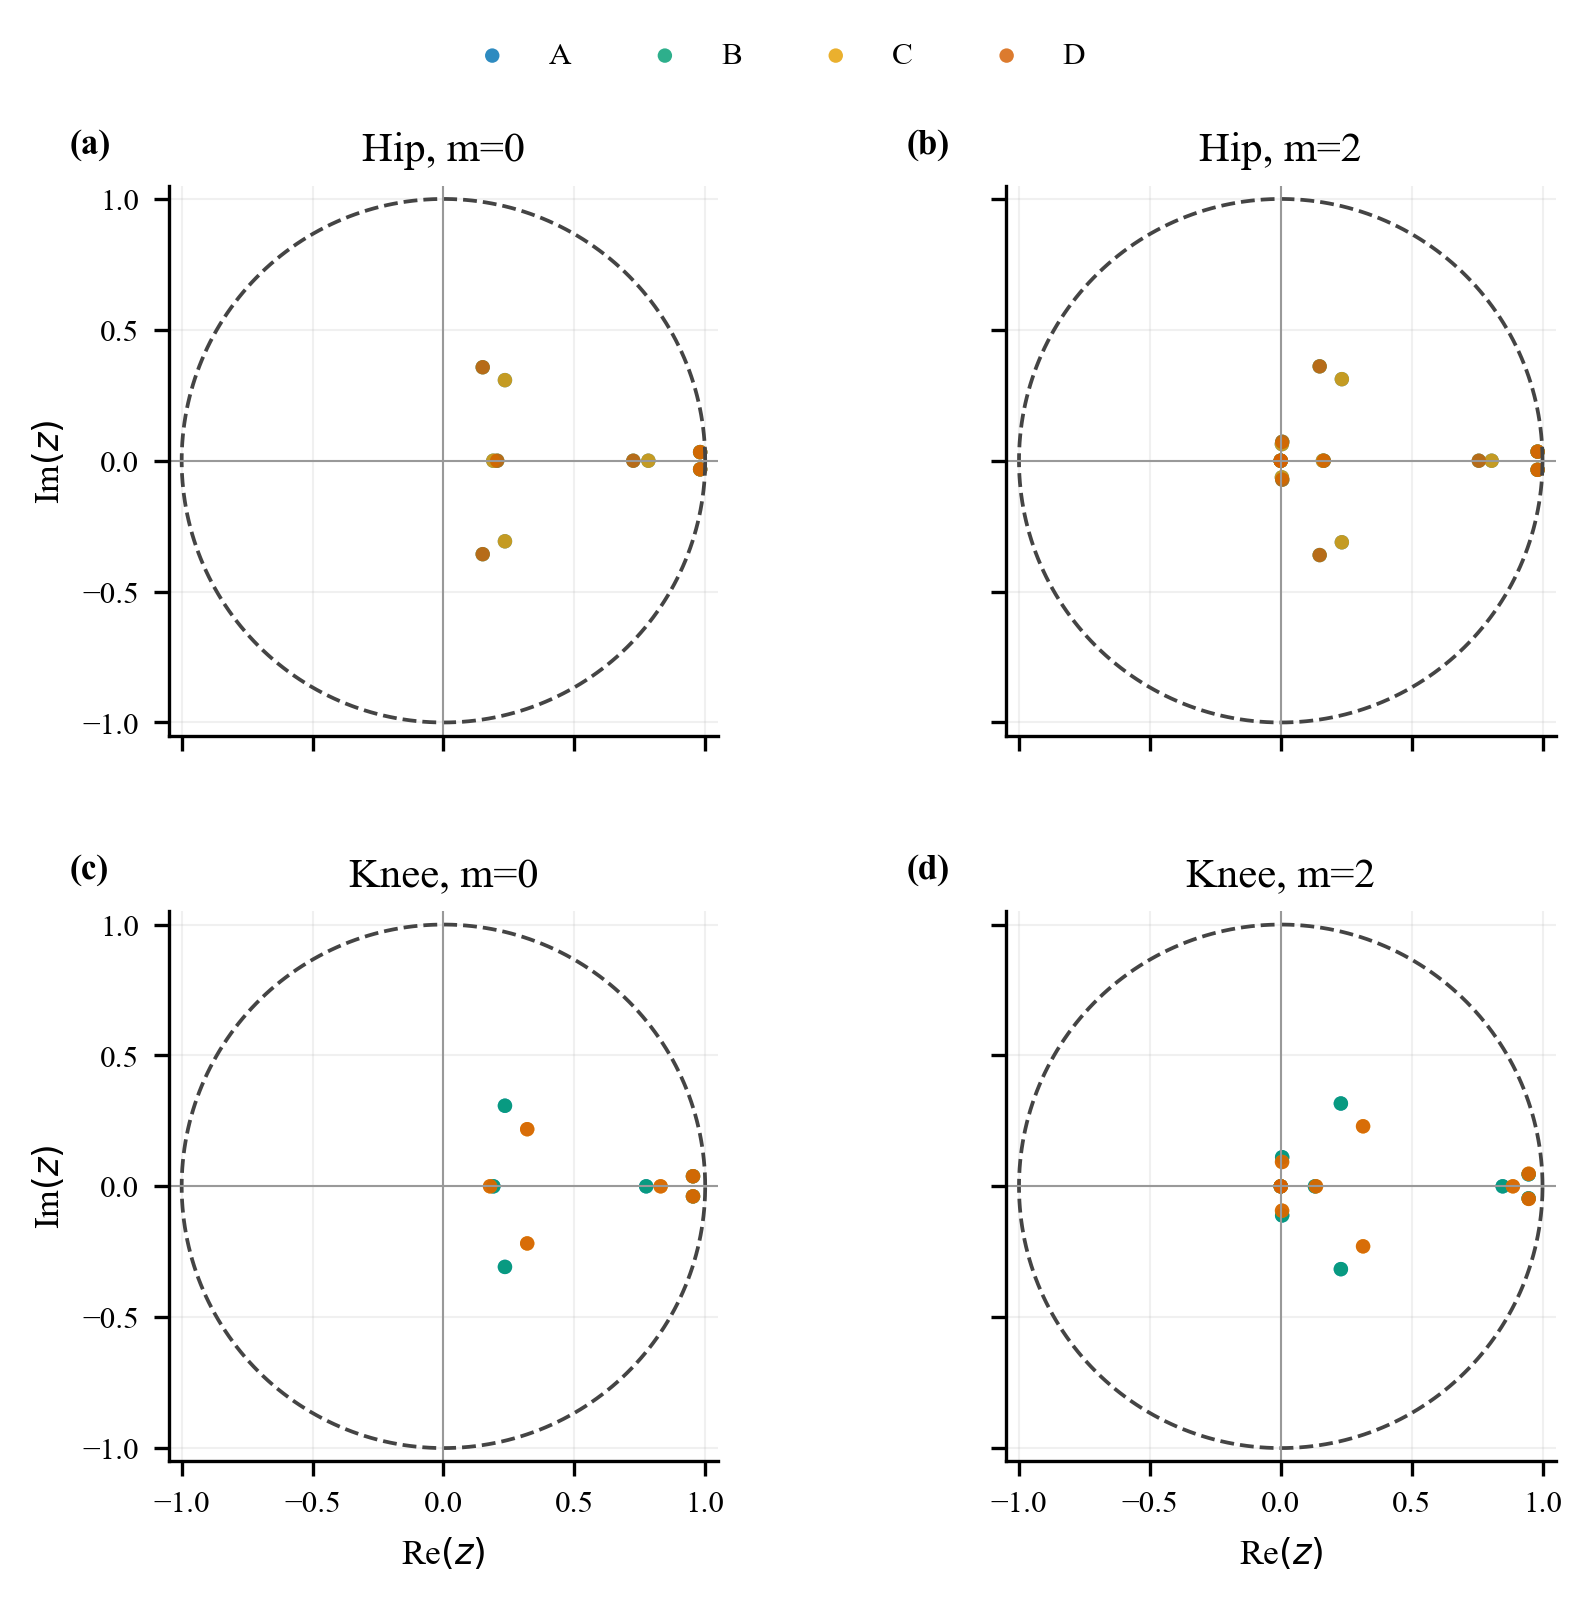
\includegraphics[keepaspectratio,alt={MuJoCo 增广闭环 z 平面极点}]{analysis_artifacts/bychen_mujoco_sweep/mujoco_deep_analysis/figures/bychen_mujoco_augmented_zplane_poles.png}}
\caption{MuJoCo 增广闭环 z 平面极点}
\end{figure}

\textbf{结论。} 在该局部辨识模型内，A（保守基线）、B（髋增强）、C（膝减弱）、D（髋增、膝减）四组、髋/膝两关节均未发现单位圆外极点。该结果只能说明局部模型未发现离散不稳定极点，不能写成实机全局稳定证明。

\subsection{8.3 扰动到误差 Bode}\label{ux6270ux52a8ux5230ux8befux5dee-bode}

\begin{longtable}[]{@{}llrrr@{}}
\toprule\noalign{}
组别 & 关节 & 峰值频率 Hz & 峰值幅值 dB & 20 Hz 幅值 dB \\
\midrule\noalign{}
\endhead
\bottomrule\noalign{}
\endlastfoot
A（保守基线） & Hip & 2.179 & -38.986 & -73.448 \\
A（保守基线） & Knee & 0.500 & -38.999 & -64.686 \\
B（髋增强） & Hip & 2.179 & -39.222 & -73.434 \\
B（髋增强） & Knee & 0.500 & -38.999 & -64.686 \\
C（膝减弱） & Knee & 0.500 & -38.253 & -64.765 \\
D（髋增、膝减） & Knee & 0.500 & -38.253 & -64.765 \\
\end{longtable}

\begin{figure}
\centering
\pandocbounded{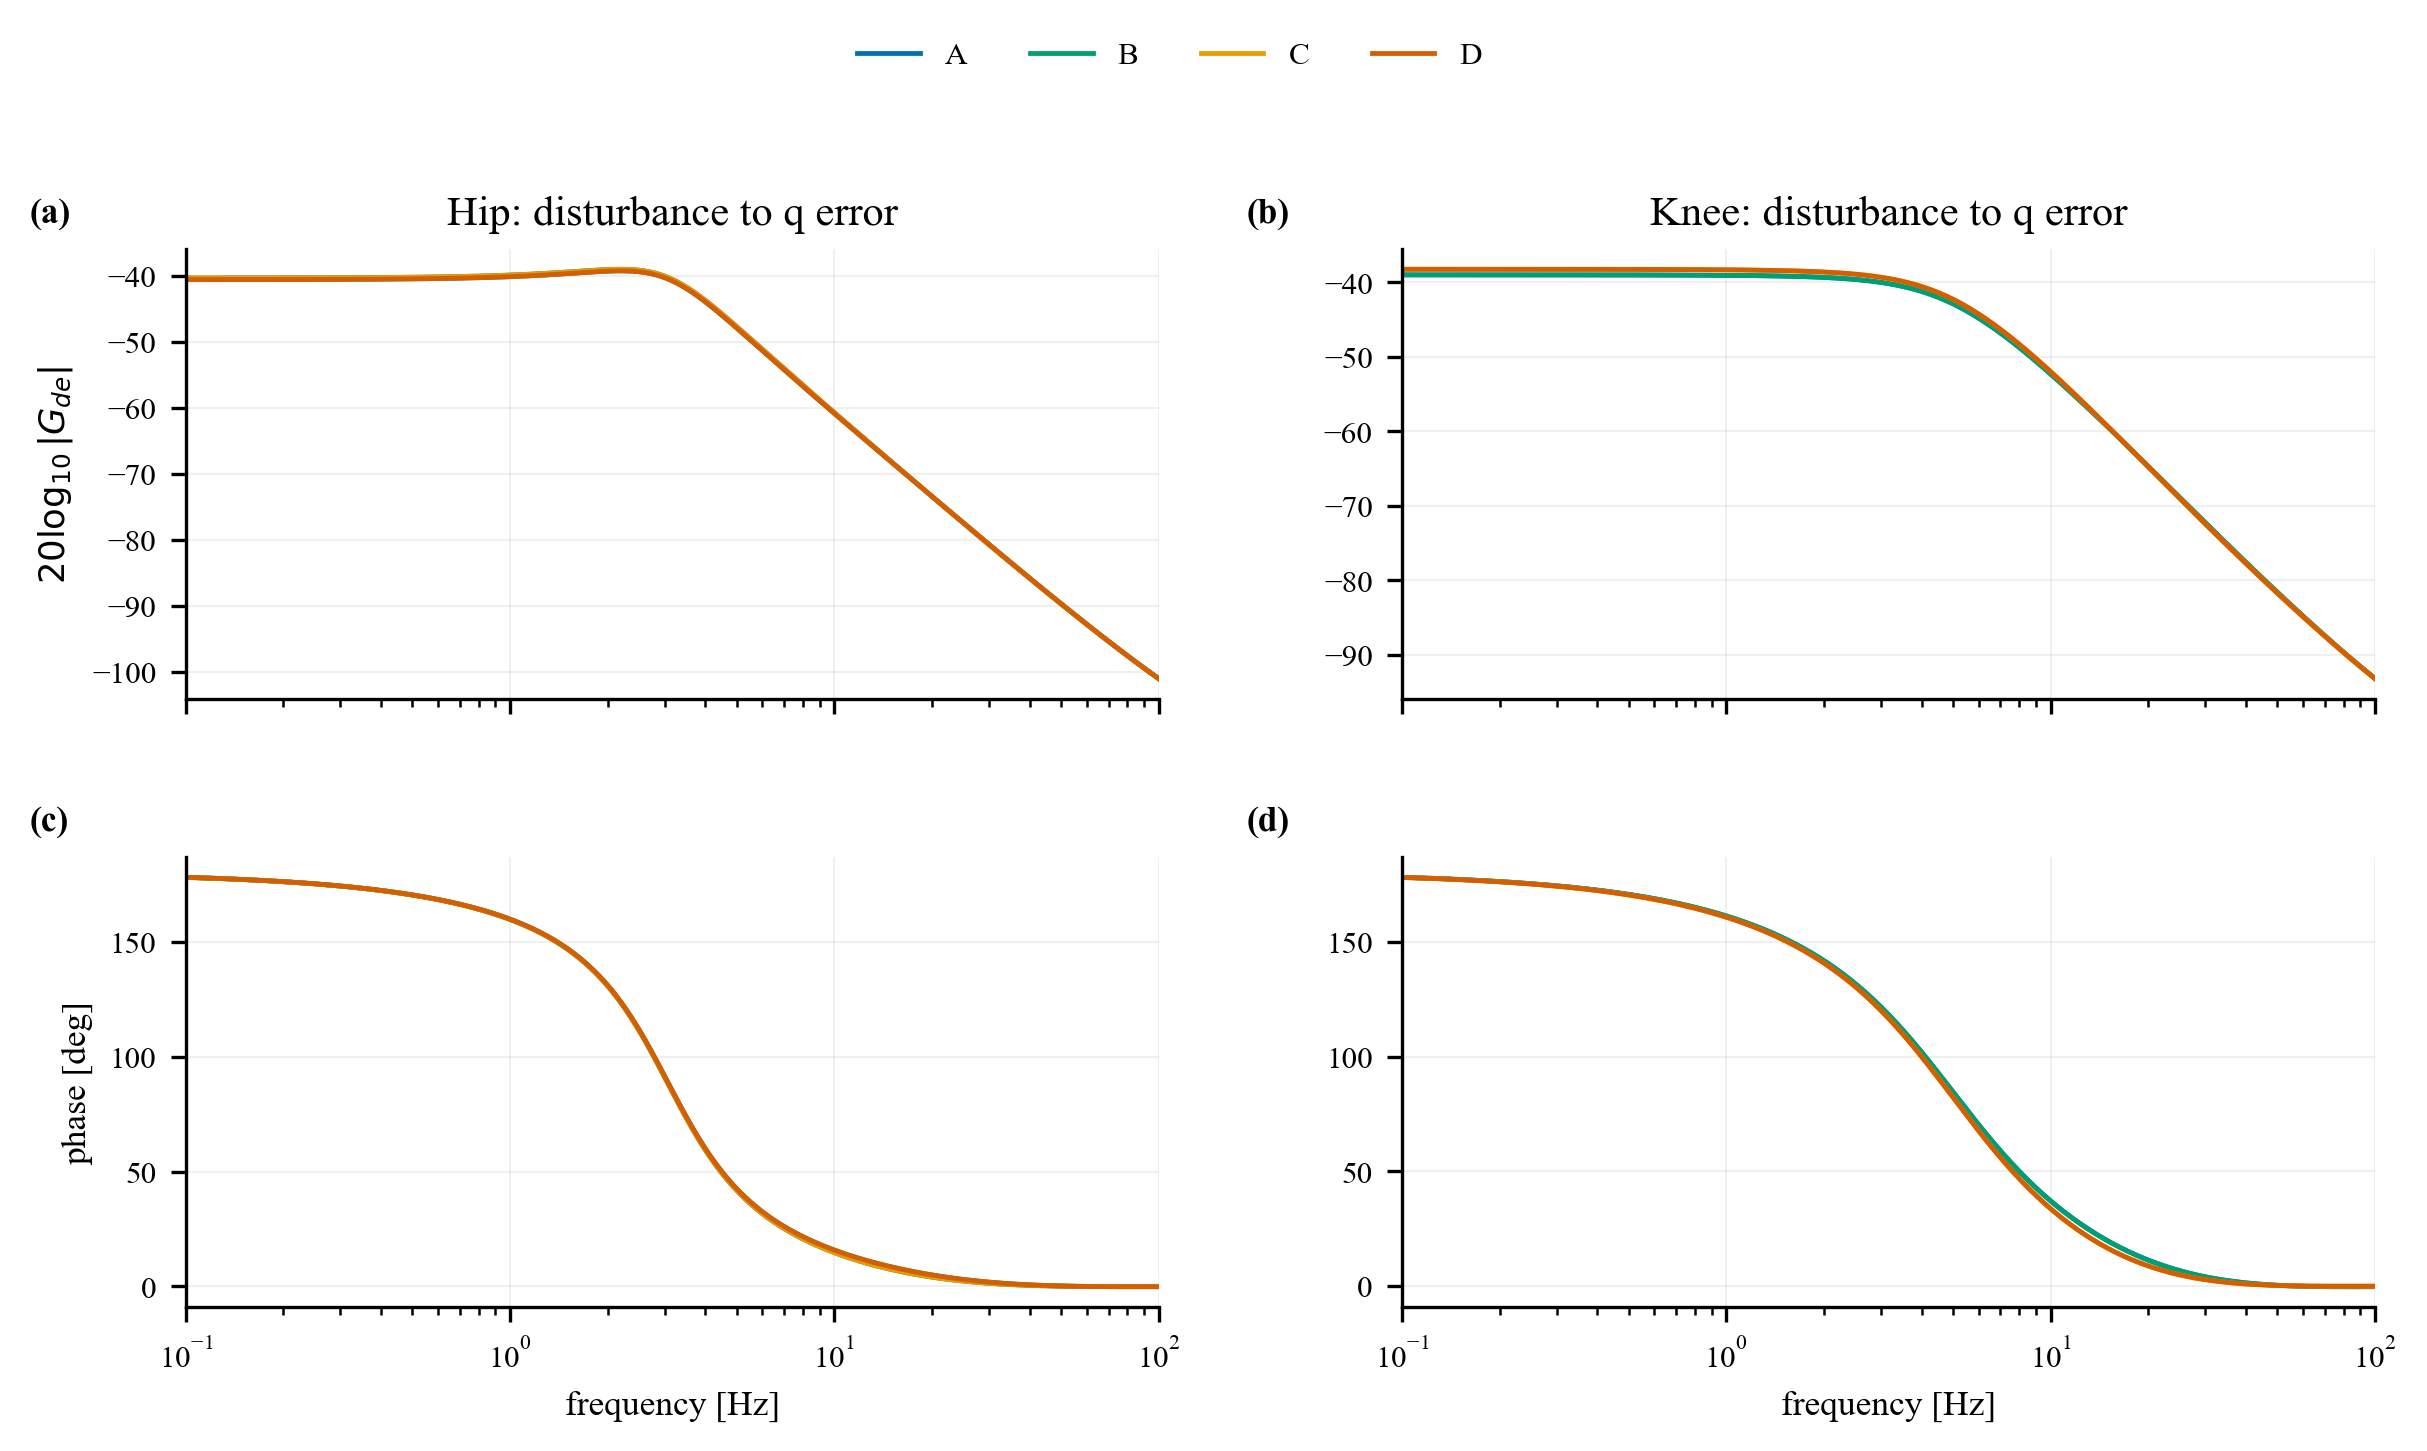
\includegraphics[keepaspectratio,alt={辨识模型扰动到误差 Bode}]{analysis_artifacts/bychen_mujoco_sweep/mujoco_deep_analysis/figures/bychen_mujoco_identified_bode_disturbance.png}}
\caption{辨识模型扰动到误差 Bode}
\end{figure}

\subsection{8.4 噪声到控制奇异值}\label{ux566aux58f0ux5230ux63a7ux5236ux5947ux5f02ux503c}

\begin{longtable}[]{@{}llrrr@{}}
\toprule\noalign{}
组别 & 关节 & 峰值频率 Hz & 峰值幅值 dB & 20 Hz 幅值 dB \\
\midrule\noalign{}
\endhead
\bottomrule\noalign{}
\endlastfoot
A（保守基线） & Hip & 4.208 & 43.161 & 41.876 \\
A（保守基线） & Knee & 44.322 & 42.020 & 41.871 \\
B（髋增强） & Hip & 4.208 & 43.163 & 41.941 \\
B（髋增强） & Knee & 44.322 & 42.020 & 41.871 \\
C（膝减弱） & Knee & 18.976 & 41.695 & 41.693 \\
D（髋增、膝减） & Knee & 18.976 & 41.695 & 41.693 \\
\end{longtable}

\begin{figure}
\centering
\pandocbounded{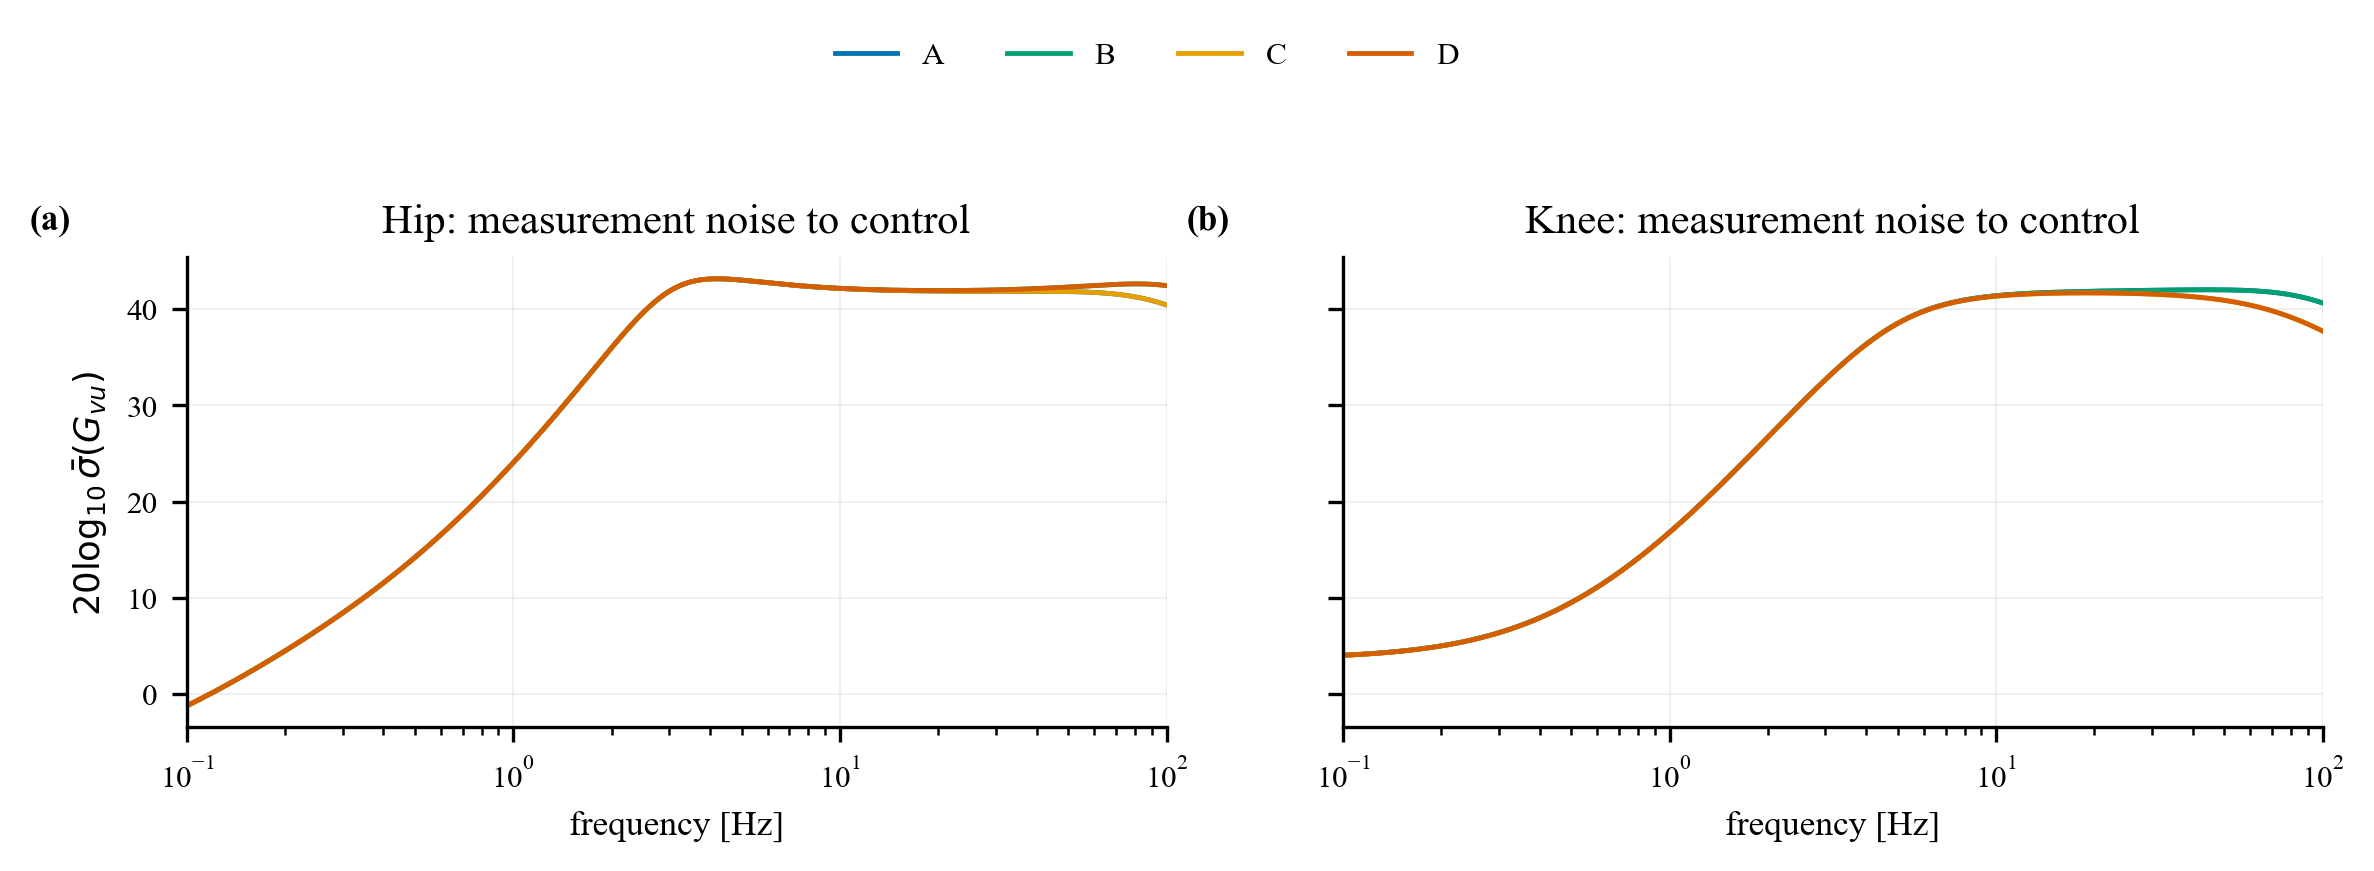
\includegraphics[keepaspectratio,alt={辨识模型测量噪声到控制奇异值}]{analysis_artifacts/bychen_mujoco_sweep/mujoco_deep_analysis/figures/bychen_mujoco_identified_noise_singular_value.png}}
\caption{辨识模型测量噪声到控制奇异值}
\end{figure}

\begin{figure}
\centering
\pandocbounded{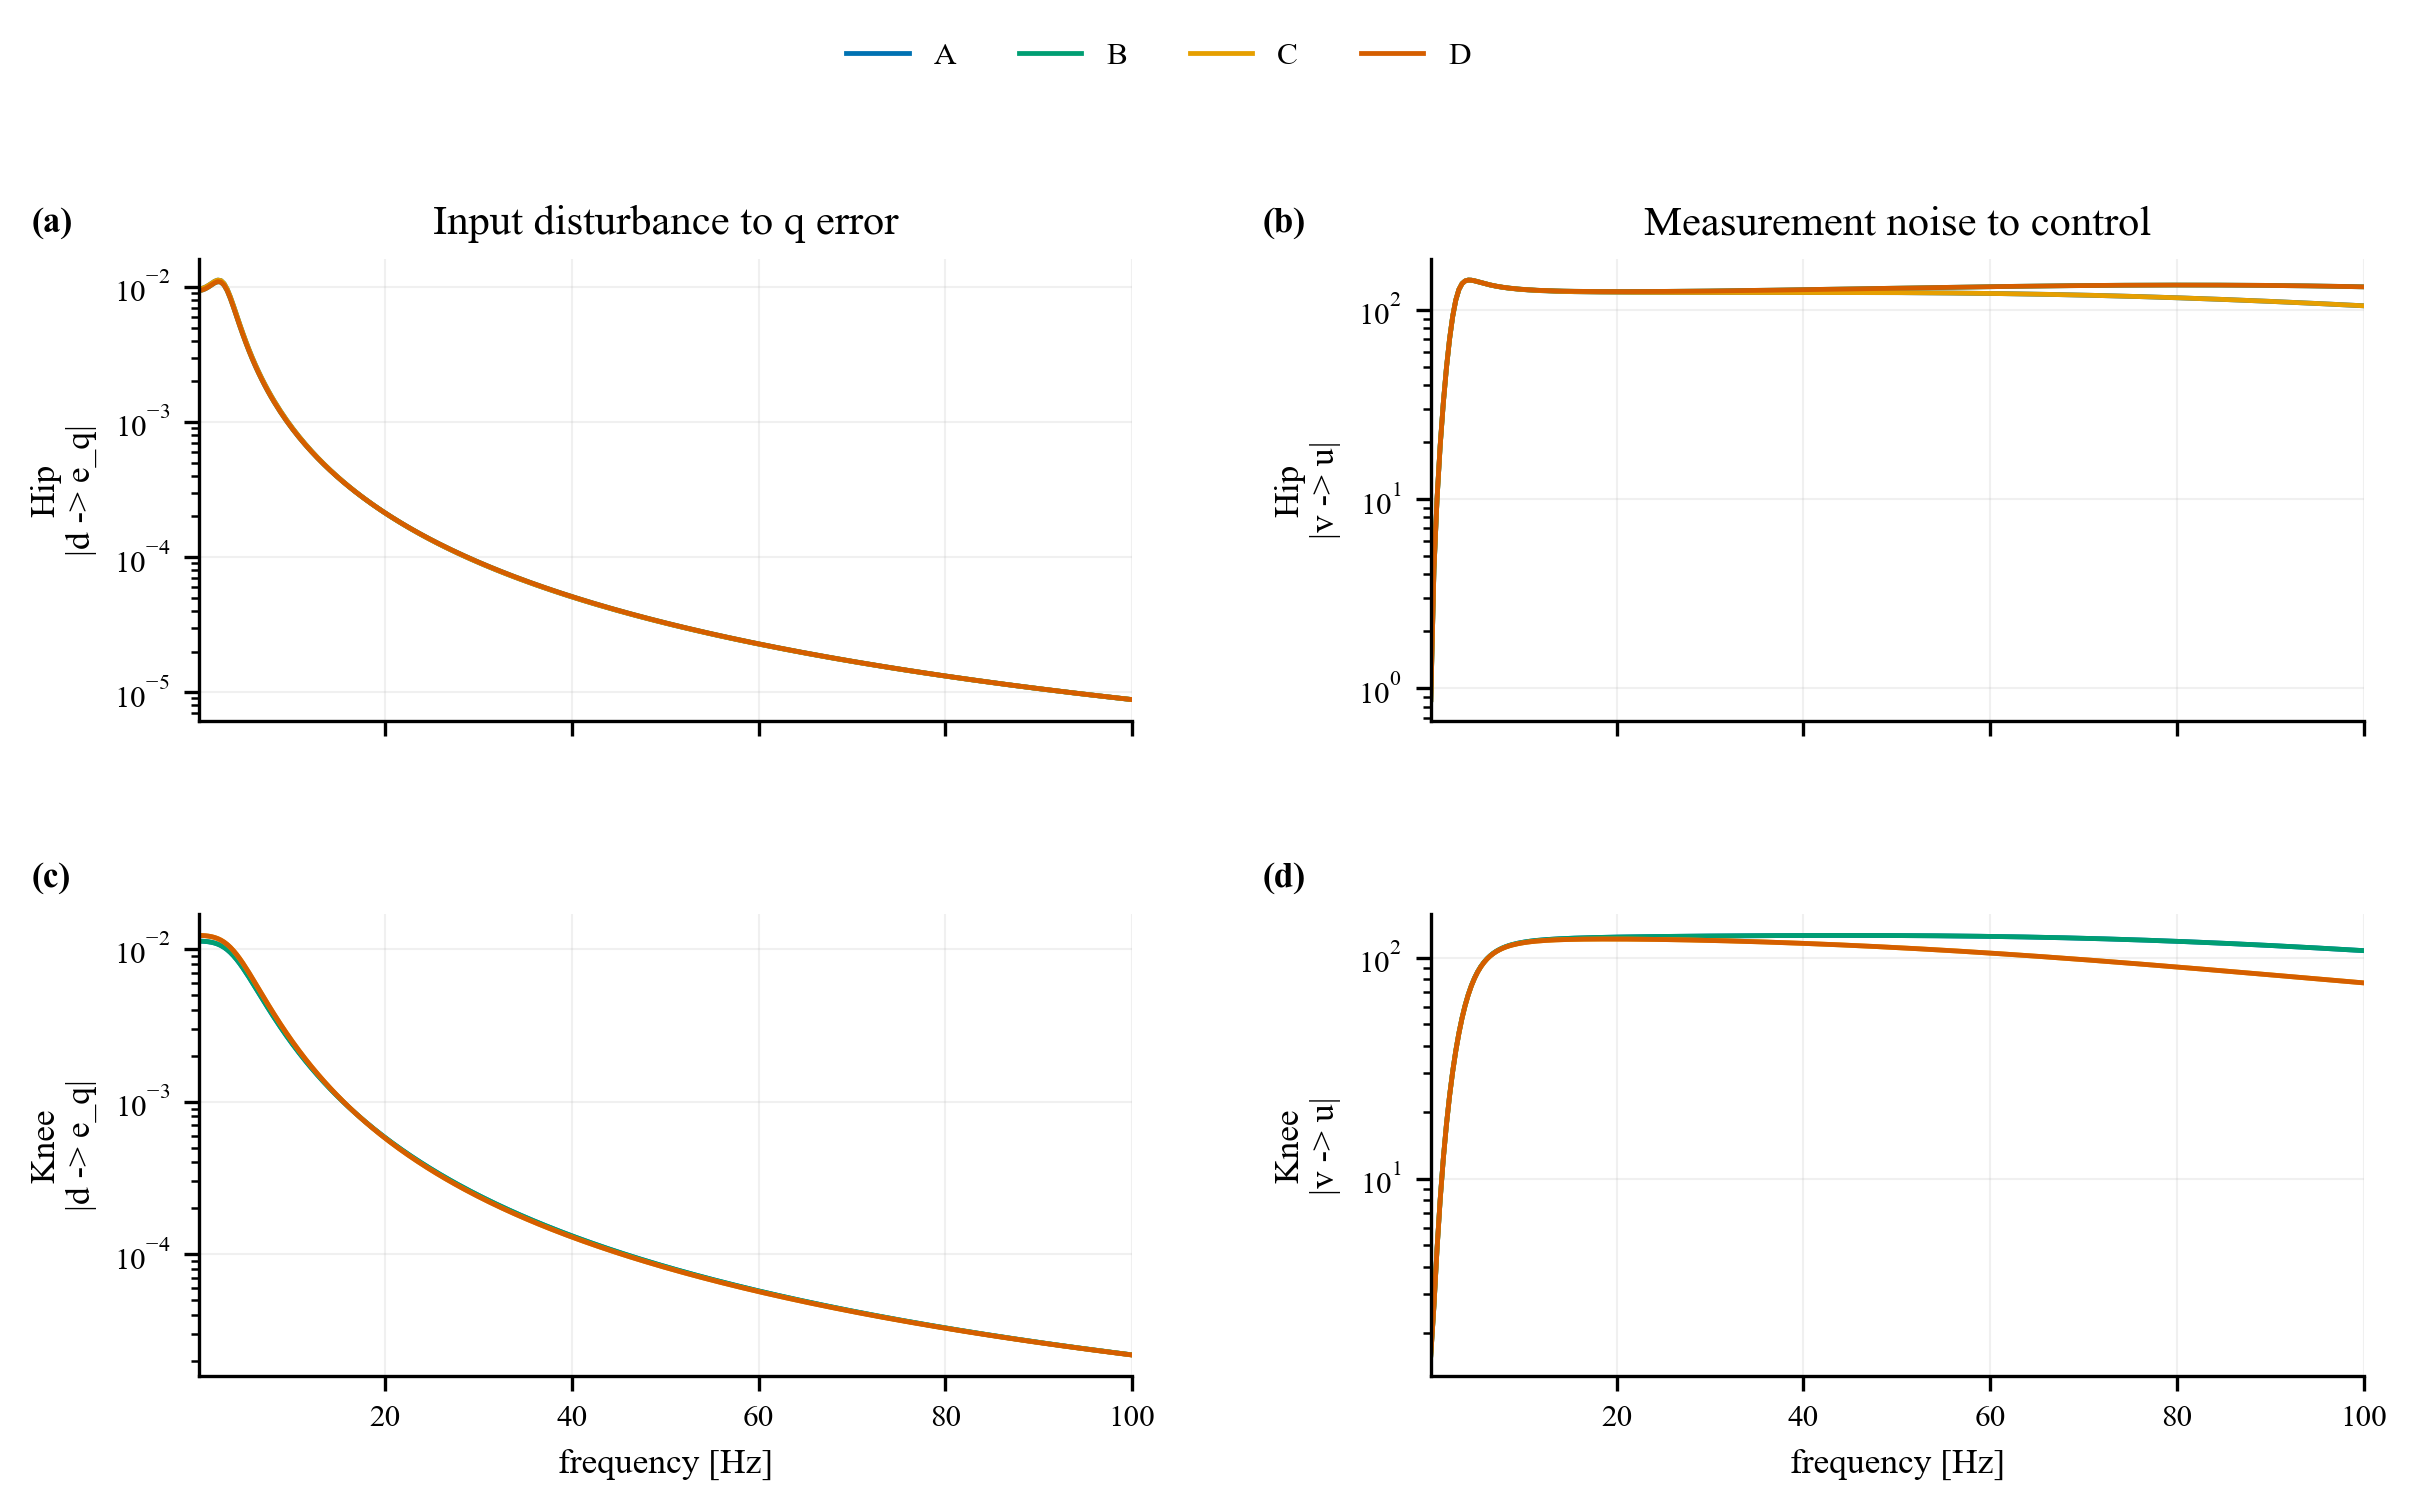
\includegraphics[keepaspectratio,alt={辨识模型增广频响}]{analysis_artifacts/bychen_mujoco_sweep/mujoco_deep_analysis/figures/bychen_mujoco_identified_augmented_frequency_response.png}}
\caption{辨识模型增广频响}
\end{figure}

\textbf{结论。} C（膝减弱）和 D（髋增、膝减）在局部模型中略降低膝测量噪声到控制输出的峰值，但没有改善膝扰动到误差的峰值增益，反而略高。这与 MuJoCo 时域结果一致：降低膝观测器倍率可减少一部分膝力矩高频活动，但代价是膝误差和协调误差变差。

\section{9. 结果图表层级}\label{ux7ed3ux679cux56feux8868ux5c42ux7ea7}

结果图表按证据层级组织。实机主结果用于支撑参数结论，频谱、力矩分解和局部模型结果用于解释机理和边界。

\begin{longtable}[]{@{}
  >{\raggedright\arraybackslash}p{(\linewidth - 4\tabcolsep) * \real{0.3333}}
  >{\raggedright\arraybackslash}p{(\linewidth - 4\tabcolsep) * \real{0.3333}}
  >{\raggedright\arraybackslash}p{(\linewidth - 4\tabcolsep) * \real{0.3333}}@{}}
\toprule\noalign{}
\begin{minipage}[b]{\linewidth}\raggedright
图表层级
\end{minipage} & \begin{minipage}[b]{\linewidth}\raggedright
内容
\end{minipage} & \begin{minipage}[b]{\linewidth}\raggedright
作用
\end{minipage} \\
\midrule\noalign{}
\endhead
\bottomrule\noalign{}
\endlastfoot
主证据 & P2D 髋、膝、协调 RMSE 与 \texttt{tau\_est} / \texttt{Delta\ tau\_est} 代价 & 给出 EID 相对 PD 的误差收益和力矩代价 \\
参数扫描 & P4D \texttt{K\_o} 与 \texttt{K\_u} 扫描，O0 作为未覆盖完整扰动窗口的失败配置单独标注 & 区分可运行候选、误差收益和补偿活动量 \\
权衡关系 & 协调 RMSE 与 \texttt{Delta\ tau\_est} / \texttt{eta\_u} RMS 的 Pareto 图和权重敏感性 & 避免把参数选择简化为单一 RMSE 最小化 \\
机制解释 & 频谱、恢复段、\texttt{eta\_u} 对齐、力矩项分解、MuJoCo 机制矩阵、局部极点和 Bode & 解释候选差异来源，并标明仿真和局部模型证据边界 \\
下一轮验证 & A/B/C/D/E 和 \texttt{KneeVelDown} 的实验矩阵 & 将候选角色区分为保守基线、误差优先候选和机制验证点 \\
\end{longtable}

\section{10. 下一轮实机实验设计}\label{ux4e0bux4e00ux8f6eux5b9eux673aux5b9eux9a8cux8bbeux8ba1}

\subsection{10.1 实验目标}\label{ux5b9eux9a8cux76eeux6807}

下一轮不再扩大共同倍率扫描，而是回答：

\begin{enumerate}
\def\labelenumi{\arabic{enumi}.}
\tightlist
\item
  单独提高髋观测器倍率是否能获得更稳妥的误差收益？
\item
  \texttt{O5+U1} 作为组合是否真的优于 \texttt{O4+U1}？
\item
  降低膝观测器倍率或膝速度观测器倍率是否能减少膝力矩活动，且不明显牺牲膝误差和协调误差？
\end{enumerate}

所有组合固定弱输入补偿：

\[
s_{u,h}=s_{u,k}=0.5,
\qquad
\alpha=0.85.
\]

\subsection{10.2 推荐矩阵}\label{ux63a8ux8350ux77e9ux9635}

\begin{longtable}[]{@{}
  >{\raggedright\arraybackslash}p{(\linewidth - 10\tabcolsep) * \real{0.1500}}
  >{\raggedright\arraybackslash}p{(\linewidth - 10\tabcolsep) * \real{0.1500}}
  >{\raggedleft\arraybackslash}p{(\linewidth - 10\tabcolsep) * \real{0.2000}}
  >{\raggedleft\arraybackslash}p{(\linewidth - 10\tabcolsep) * \real{0.2000}}
  >{\raggedright\arraybackslash}p{(\linewidth - 10\tabcolsep) * \real{0.1500}}
  >{\raggedright\arraybackslash}p{(\linewidth - 10\tabcolsep) * \real{0.1500}}@{}}
\toprule\noalign{}
\begin{minipage}[b]{\linewidth}\raggedright
优先级
\end{minipage} & \begin{minipage}[b]{\linewidth}\raggedright
配置
\end{minipage} & \begin{minipage}[b]{\linewidth}\raggedleft
髋 \texttt{s\_o}
\end{minipage} & \begin{minipage}[b]{\linewidth}\raggedleft
膝 \texttt{s\_o}
\end{minipage} & \begin{minipage}[b]{\linewidth}\raggedright
目的
\end{minipage} & \begin{minipage}[b]{\linewidth}\raggedright
证据等级
\end{minipage} \\
\midrule\noalign{}
\endhead
\bottomrule\noalign{}
\endlastfoot
必做 & A：\texttt{O4+U1} 保守基线，即标称观测器倍率 + U1 弱输入补偿 & 1.00 & 1.00 & 已实测保守基线，同批次对照 & 已实机支持，需同批复测 \\
必做 & B：髋增强，即只提高髋观测器倍率 & 1.25 & 1.00 & 单独验证提高髋 \texttt{K\_o} 的收益 & MuJoCo 迹象，待实机 \\
必做 & E：\texttt{O5+U1}，即髋膝共同高观测器倍率 + U1 弱输入补偿 & 1.25 & 1.25 & 验证``误差优先候选''的实际实机表现 & 待实机 \\
机制验证 & C：膝减弱，即只降低膝观测器倍率 & 1.00 & 0.75 & 验证降低膝 \texttt{K\_o} 是否减少膝力矩活动 & 待实机 \\
机制验证 & D：髋增、膝减，即髋观测器倍率提高、膝观测器倍率降低 & 1.25 & 0.75 & 直接验证``髋增、膝减''假设 & MuJoCo 迹象，待实机 \\
机制验证 & \texttt{KneeVelDown}：只降低膝速度观测器通道 & 髋 1.00 & 膝位置 1.00，膝速度 0.75 & 判断膝力矩活动是否主要来自速度残差通道 & MuJoCo 迹象，待实机 \\
\end{longtable}

如果上机时间有限，先做 A（保守基线）、B（髋增强）和 E（\texttt{O5+U1}）；若必须直接回答非对称调参问题，则做 A/B/C/D 的 2x2 矩阵，其中 C 和 D 分别隔离``膝减弱''与``髋增、膝减''的影响。

\subsection{10.3 每组报告指标}\label{ux6bcfux7ec4ux62a5ux544aux6307ux6807}

每组先做无扰动安全门槛，再做 P2D 软件扰动，每组至少 5 次完整重复。必须报告：

\begin{itemize}
\tightlist
\item
  髋、膝、协调窗口 RMSE；
\item
  髋、膝、协调峰值误差；
\item
  恢复段 RMSE 和恢复时间；
\item
  髋/膝 \texttt{tau\_est} RMS；
\item
  髋/膝 \texttt{Delta\ tau\_est} RMS；
\item
  分频段力矩功率；
\item
  饱和次数、速度超限、完整运行率。
\end{itemize}

\section{11. 结论边界与表述约束}\label{ux7ed3ux8bbaux8fb9ux754cux4e0eux8868ux8ff0ux7ea6ux675f}

本报告的结论必须与证据等级一致。实机日志、MuJoCo 机制筛查和局部线性模型分别支持不同强度的表述。

\begin{longtable}[]{@{}
  >{\raggedright\arraybackslash}p{(\linewidth - 4\tabcolsep) * \real{0.3333}}
  >{\raggedright\arraybackslash}p{(\linewidth - 4\tabcolsep) * \real{0.3333}}
  >{\raggedright\arraybackslash}p{(\linewidth - 4\tabcolsep) * \real{0.3333}}@{}}
\toprule\noalign{}
\begin{minipage}[b]{\linewidth}\raggedright
主题
\end{minipage} & \begin{minipage}[b]{\linewidth}\raggedright
证据支持的表述
\end{minipage} & \begin{minipage}[b]{\linewidth}\raggedright
不支持的表述
\end{minipage} \\
\midrule\noalign{}
\endhead
\bottomrule\noalign{}
\endlastfoot
EID 相对 PD & P2D 中 EID 改善髋窗口 RMSE、协调窗口 RMSE 和峰值误差，但膝窗口 RMSE 上升，且力矩活动增加 & EID 在扰动下所有指标均优于 PD \\
\texttt{K\_o} 扫描 & 髋膝共同增大 \texttt{K\_o} 时，P4D 扰动窗口 RMSE 下降 & 已证明逐关节非对称调参优于共同倍率扫描 \\
\texttt{K\_u} 扫描 & 增大 \texttt{K\_u} 主要放大 \texttt{eta\_u} 活动量，对窗口 RMSE 收益有限 & 继续增大 \texttt{K\_u} 可以解决力矩波动或显著提高抗扰性能 \\
\texttt{O5+U1} & \texttt{O5+U1} 是待实机验证的误差优先组合候选 & \texttt{O5+U1} 已经由本轮 P4D 实机直接验证 \\
A/B/C/D/E 矩阵 & A 是保守基线；B 和 E 是优先验证候选；C、D、\texttt{KneeVelDown} 用于检验膝力矩活动机制 & D 或 \texttt{KneeVelDown} 可预先写成最优参数 \\
MuJoCo 与局部模型 & 可用于候选压缩、机制解释和风险提示 & 可替代实机安全裕度、实机稳定性证明或真实物理外扰验证 \\
\end{longtable}

\section{附录 A：已生成图表清单}\label{ux9644ux5f55-aux5df2ux751fux6210ux56feux8868ux6e05ux5355}

\subsection{A.1 实机离线分析图}\label{a.1-ux5b9eux673aux79bbux7ebfux5206ux6790ux56fe}

\begin{longtable}[]{@{}
  >{\raggedright\arraybackslash}p{(\linewidth - 2\tabcolsep) * \real{0.5000}}
  >{\raggedright\arraybackslash}p{(\linewidth - 2\tabcolsep) * \real{0.5000}}@{}}
\toprule\noalign{}
\begin{minipage}[b]{\linewidth}\raggedright
图
\end{minipage} & \begin{minipage}[b]{\linewidth}\raggedright
路径
\end{minipage} \\
\midrule\noalign{}
\endhead
\bottomrule\noalign{}
\endlastfoot
P4D 增益扫描 & \texttt{analysis\_artifacts/bychen\_answer/figures/bychen\_p4d\_gain\_scans.png} \\
P2D 全重复频谱 & \texttt{analysis\_artifacts/bychen\_answer/figures/bychen\_p2d\_all\_repeat\_spectrum.png} \\
P2D 扰动窗口频谱 & \texttt{analysis\_artifacts/bychen\_answer/figures/bychen\_p2d\_disturbance\_spectrum.png} \\
P4D 候选频谱 & \texttt{analysis\_artifacts/bychen\_answer/figures/bychen\_p4d\_candidate\_spectrum.png} \\
P2D 恢复段统计 & \texttt{analysis\_artifacts/bychen\_answer/figures/bychen\_p2d\_window\_recovery.png} \\
P4D 候选窗口统计 & \texttt{analysis\_artifacts/bychen\_answer/figures/bychen\_p4d\_candidate\_windows.png} \\
\texttt{eta\_u} 与扰动对齐 & \texttt{analysis\_artifacts/bychen\_answer/figures/bychen\_eta\_disturbance\_alignment.png} \\
力矩项分解 & \texttt{analysis\_artifacts/bychen\_answer/figures/bychen\_force\_decomposition.png} \\
Pareto 图 & \texttt{analysis\_artifacts/bychen\_answer/figures/bychen\_tradeoff\_pareto.png} \\
权重敏感性 & \texttt{analysis\_artifacts/bychen\_answer/figures/bychen\_multiobjective\_sensitivity.png} \\
简化极点图 & \texttt{analysis\_artifacts/bychen\_answer/figures/bychen\_augmented\_pole\_grid.png} \\
简化频响 & \texttt{analysis\_artifacts/bychen\_answer/figures/bychen\_augmented\_frequency\_response.png} \\
\end{longtable}

\subsection{A.2 MuJoCo 机制矩阵图}\label{a.2-mujoco-ux673aux5236ux77e9ux9635ux56fe}

\begin{longtable}[]{@{}
  >{\raggedright\arraybackslash}p{(\linewidth - 2\tabcolsep) * \real{0.5000}}
  >{\raggedright\arraybackslash}p{(\linewidth - 2\tabcolsep) * \real{0.5000}}@{}}
\toprule\noalign{}
\begin{minipage}[b]{\linewidth}\raggedright
图
\end{minipage} & \begin{minipage}[b]{\linewidth}\raggedright
路径
\end{minipage} \\
\midrule\noalign{}
\endhead
\bottomrule\noalign{}
\endlastfoot
候选 Pareto & \texttt{analysis\_artifacts/bychen\_mujoco\_mechanism\_completion/figures/mujoco\_mechanism\_candidate\_pareto.png} \\
候选频谱摘要 & \texttt{analysis\_artifacts/bychen\_mujoco\_mechanism\_completion/figures/mujoco\_mechanism\_spectrum\_summary.png} \\
结构消融 & \texttt{analysis\_artifacts/bychen\_mujoco\_mechanism\_completion/figures/mujoco\_mechanism\_structure\_ablation.png} \\
残差 \texttt{lambda} 扫描 & \texttt{analysis\_artifacts/bychen\_mujoco\_mechanism\_completion/figures/mujoco\_mechanism\_residual\_lambda.png} \\
\end{longtable}

\subsection{A.3 MuJoCo 深度分析图}\label{a.3-mujoco-ux6df1ux5ea6ux5206ux6790ux56fe}

\begin{longtable}[]{@{}
  >{\raggedright\arraybackslash}p{(\linewidth - 2\tabcolsep) * \real{0.5000}}
  >{\raggedright\arraybackslash}p{(\linewidth - 2\tabcolsep) * \real{0.5000}}@{}}
\toprule\noalign{}
\begin{minipage}[b]{\linewidth}\raggedright
图
\end{minipage} & \begin{minipage}[b]{\linewidth}\raggedright
路径
\end{minipage} \\
\midrule\noalign{}
\endhead
\bottomrule\noalign{}
\endlastfoot
日志 PSD & \texttt{analysis\_artifacts/bychen\_mujoco\_sweep/mujoco\_deep\_analysis/figures/bychen\_mujoco\_log\_psd.png} \\
扰动 coherence & \texttt{analysis\_artifacts/bychen\_mujoco\_sweep/mujoco\_deep\_analysis/figures/bychen\_mujoco\_disturbance\_coherence.png} \\
经验 FRF/Bode & \texttt{analysis\_artifacts/bychen\_mujoco\_sweep/mujoco\_deep\_analysis/figures/bychen\_mujoco\_empirical\_frf\_bode.png} \\
z 平面极点 & \texttt{analysis\_artifacts/bychen\_mujoco\_sweep/mujoco\_deep\_analysis/figures/bychen\_mujoco\_augmented\_zplane\_poles.png} \\
扰动到误差 Bode & \texttt{analysis\_artifacts/bychen\_mujoco\_sweep/mujoco\_deep\_analysis/figures/bychen\_mujoco\_identified\_bode\_disturbance.png} \\
噪声到控制奇异值 & \texttt{analysis\_artifacts/bychen\_mujoco\_sweep/mujoco\_deep\_analysis/figures/bychen\_mujoco\_identified\_noise\_singular\_value.png} \\
辨识模型增广频响 & \texttt{analysis\_artifacts/bychen\_mujoco\_sweep/mujoco\_deep\_analysis/figures/bychen\_mujoco\_identified\_augmented\_frequency\_response.png} \\
\end{longtable}

\section{附录 B：数据与脚本产物}\label{ux9644ux5f55-bux6570ux636eux4e0eux811aux672cux4ea7ux7269}

\subsection{B.1 实机离线分析}\label{b.1-ux5b9eux673aux79bbux7ebfux5206ux6790}

\begin{Shaded}
\begin{Highlighting}[]
\NormalTok{analysis\_artifacts/bychen\_answer/}
\NormalTok{analysis\_artifacts/real\_p2d\_p4d\_summary/}
\end{Highlighting}
\end{Shaded}

关键表：

\begin{itemize}
\tightlist
\item
  \texttt{bychen\_p2d\_spectrum\_peaks.csv}
\item
  \texttt{bychen\_p4d\_candidate\_spectrum\_peaks.csv}
\item
  \texttt{bychen\_eta\_disturbance\_alignment\_summary.csv}
\item
  \texttt{bychen\_force\_decomposition\_summary.csv}
\item
  \texttt{bychen\_tradeoff\_points.csv}
\item
  \texttt{bychen\_multiobjective\_ranking.csv}
\end{itemize}

\subsection{B.2 MuJoCo 候选与机制矩阵}\label{b.2-mujoco-ux5019ux9009ux4e0eux673aux5236ux77e9ux9635}

\begin{Shaded}
\begin{Highlighting}[]
\NormalTok{analysis\_artifacts/bychen\_mujoco\_sweep/}
\NormalTok{analysis\_artifacts/bychen\_mujoco\_mechanism\_completion/}
\end{Highlighting}
\end{Shaded}

关键表：

\begin{itemize}
\tightlist
\item
  \texttt{bychen\_mujoco\_metrics\_with\_relative.csv}
\item
  \texttt{mujoco\_deep\_analysis/frequency/bychen\_mujoco\_psd\_peaks.csv}
\item
  \texttt{mujoco\_deep\_analysis/frequency/bychen\_mujoco\_coherence\_summary.csv}
\item
  \texttt{mujoco\_deep\_analysis/frequency/bychen\_mujoco\_empirical\_frf\_summary.csv}
\item
  \texttt{mujoco\_deep\_analysis/linearized/bychen\_mujoco\_identified\_plants.csv}
\item
  \texttt{mujoco\_deep\_analysis/linearized/bychen\_mujoco\_augmented\_poles.csv}
\item
  \texttt{mujoco\_deep\_analysis/linearized/bychen\_mujoco\_augmented\_frequency\_response.csv}
\item
  \texttt{mujoco\_mechanism\_metrics.csv}
\item
  \texttt{mujoco\_mechanism\_metrics\_with\_relative.csv}
\item
  \texttt{mujoco\_mechanism\_frequency\_summary.csv}
\item
  \texttt{mujoco\_mechanism\_completion\_summary.md}
\end{itemize}

\section{附录 C：可复现命令}\label{ux9644ux5f55-cux53efux590dux73b0ux547dux4ee4}

已有基础绘图和分析脚本：

\begin{Shaded}
\begin{Highlighting}[]
\ExtensionTok{python}\NormalTok{ scripts/make\_bychen\_answer\_figures.py}
\ExtensionTok{python}\NormalTok{ scripts/run\_bychen\_full\_analysis.py}
\end{Highlighting}
\end{Shaded}

MuJoCo 机制矩阵：

\begin{Shaded}
\begin{Highlighting}[]
\FunctionTok{cmake} \AttributeTok{{-}{-}build}\NormalTok{ build }\AttributeTok{{-}{-}config}\NormalTok{ Debug }\AttributeTok{{-}{-}target}\NormalTok{ h1\_controller\_stepper}
\ExtensionTok{python}\NormalTok{ scripts/run\_bychen\_mujoco\_mechanism\_completion.py }\AttributeTok{{-}{-}skip{-}existing}
\end{Highlighting}
\end{Shaded}

以上命令对应的输出已经纳入本报告。后续若重跑，应检查数值是否与本报告表格一致；若不一致，应以最新同一批次产物更新图表和结论。
